\documentclass[twoside]{book}

% Packages required by doxygen
\usepackage{fixltx2e}
\usepackage{calc}
\usepackage{doxygen}
\usepackage[export]{adjustbox} % also loads graphicx
\usepackage{graphicx}
\usepackage[utf8]{inputenc}
\usepackage{makeidx}
\usepackage{multicol}
\usepackage{multirow}
\PassOptionsToPackage{warn}{textcomp}
\usepackage{textcomp}
\usepackage[nointegrals]{wasysym}
\usepackage[table]{xcolor}

% Font selection
\usepackage[T1]{fontenc}
\usepackage[scaled=.90]{helvet}
\usepackage{courier}
\usepackage{amssymb}
\usepackage{sectsty}
\renewcommand{\familydefault}{\sfdefault}
\allsectionsfont{%
  \fontseries{bc}\selectfont%
  \color{darkgray}%
}
\renewcommand{\DoxyLabelFont}{%
  \fontseries{bc}\selectfont%
  \color{darkgray}%
}
\newcommand{\+}{\discretionary{\mbox{\scriptsize$\hookleftarrow$}}{}{}}

% Page & text layout
\usepackage{geometry}
\geometry{%
  a4paper,%
  top=2.5cm,%
  bottom=2.5cm,%
  left=2.5cm,%
  right=2.5cm%
}
\tolerance=750
\hfuzz=15pt
\hbadness=750
\setlength{\emergencystretch}{15pt}
\setlength{\parindent}{0cm}
\setlength{\parskip}{3ex plus 2ex minus 2ex}
\makeatletter
\renewcommand{\paragraph}{%
  \@startsection{paragraph}{4}{0ex}{-1.0ex}{1.0ex}{%
    \normalfont\normalsize\bfseries\SS@parafont%
  }%
}
\renewcommand{\subparagraph}{%
  \@startsection{subparagraph}{5}{0ex}{-1.0ex}{1.0ex}{%
    \normalfont\normalsize\bfseries\SS@subparafont%
  }%
}
\makeatother

% Headers & footers
\usepackage{fancyhdr}
\pagestyle{fancyplain}
\fancyhead[LE]{\fancyplain{}{\bfseries\thepage}}
\fancyhead[CE]{\fancyplain{}{}}
\fancyhead[RE]{\fancyplain{}{\bfseries\leftmark}}
\fancyhead[LO]{\fancyplain{}{\bfseries\rightmark}}
\fancyhead[CO]{\fancyplain{}{}}
\fancyhead[RO]{\fancyplain{}{\bfseries\thepage}}
\fancyfoot[LE]{\fancyplain{}{}}
\fancyfoot[CE]{\fancyplain{}{}}
\fancyfoot[RE]{\fancyplain{}{\bfseries\scriptsize Generated by Doxygen }}
\fancyfoot[LO]{\fancyplain{}{\bfseries\scriptsize Generated by Doxygen }}
\fancyfoot[CO]{\fancyplain{}{}}
\fancyfoot[RO]{\fancyplain{}{}}
\renewcommand{\footrulewidth}{0.4pt}
\renewcommand{\chaptermark}[1]{%
  \markboth{#1}{}%
}
\renewcommand{\sectionmark}[1]{%
  \markright{\thesection\ #1}%
}

% Indices & bibliography
\usepackage{natbib}
\usepackage[titles]{tocloft}
\setcounter{tocdepth}{3}
\setcounter{secnumdepth}{5}
\makeindex

% Hyperlinks (required, but should be loaded last)
\usepackage{ifpdf}
\ifpdf
  \usepackage[pdftex,pagebackref=true]{hyperref}
\else
  \usepackage[ps2pdf,pagebackref=true]{hyperref}
\fi
\hypersetup{%
  colorlinks=true,%
  linkcolor=blue,%
  citecolor=blue,%
  unicode%
}

% Custom commands
\newcommand{\clearemptydoublepage}{%
  \newpage{\pagestyle{empty}\cleardoublepage}%
}

\usepackage{caption}
\captionsetup{labelsep=space,justification=centering,font={bf},singlelinecheck=off,skip=4pt,position=top}

%===== C O N T E N T S =====

\begin{document}

% Titlepage & ToC
\hypersetup{pageanchor=false,
             bookmarksnumbered=true,
             pdfencoding=unicode
            }
\pagenumbering{roman}
\begin{titlepage}
\vspace*{7cm}
\begin{center}%
{\Large Towards Autonomy Perception Library (T\+A\+PL) }\\
\vspace*{1cm}
{\large Generated by Doxygen 1.8.11}\\
\end{center}
\end{titlepage}
\clearemptydoublepage
\tableofcontents
\clearemptydoublepage
\pagenumbering{arabic}
\hypersetup{pageanchor=true}

%--- Begin generated contents ---
\chapter{Towards Autonomy Perception Library (T\+A\+PL)}
\label{index}\hypertarget{index}{}Goal of this library is to provide an easy and quick way of implementing perception pipelines.



\subsection*{Examples of Perception Task}

\paragraph*{Visual Odometry for a sequence of Monocular camera images}


\begin{DoxyItemize}
\item All the A\+PI has been provided in {\itshape src/cv\+Engine.\+cpp}. See usage in {\itshape examples/mono\+V\+O.\+cpp}
\end{DoxyItemize}



\paragraph*{Visual Odometry for a sequence of Stereo camera images}


\begin{DoxyItemize}
\item Under development
\end{DoxyItemize}

\paragraph*{Euclidean Clustering within a point-\/cloud using kd-\/tree for storing points.}


\begin{DoxyItemize}
\item C++ implementation of R\+A\+N\+S\+AC for ground segmentation, kd-\/tree and euclidean clustering in {\itshape src/pt\+Engine.\+cpp}
\end{DoxyItemize}



\paragraph*{Image Feature Detection and Tracking}


\begin{DoxyItemize}
\item C++ implementation in {\itshape src/cv\+Engine.\+cpp}
\end{DoxyItemize}



\paragraph*{R\+A\+N\+S\+AC for line and plane fitting}


\begin{DoxyItemize}
\item C++ implementation of R\+A\+N\+S\+AC for line and plane fitting using both S\+VD and least-\/square methods are provided in {\itshape cve/pt\+Engine.\+cpp} which can be simply used as an A\+PI.
\end{DoxyItemize}

\tabulinesep=1mm
\begin{longtabu} spread 0pt [c]{*2{|X[-1]}|}
\hline
\rowcolor{\tableheadbgcolor}\PBS\centering {\bf Line Fitting using R\+A\+N\+S\+AC }&\PBS\centering {\bf Plane Fitting using R\+A\+N\+S\+AC  }\\\cline{1-2}
\endfirsthead
\hline
\endfoot
\hline
\rowcolor{\tableheadbgcolor}\PBS\centering {\bf Line Fitting using R\+A\+N\+S\+AC }&\PBS\centering {\bf Plane Fitting using R\+A\+N\+S\+AC  }\\\cline{1-2}
\endhead
\PBS\centering  &\PBS\centering \\\cline{1-2}
\end{longtabu}
\subsection*{Prerequisites}


\begin{DoxyItemize}
\item C\+Make $>$= 3.\+5
\item Open\+CV $>$= 4.\+1
\item P\+CL $>$= 1.\+2
\end{DoxyItemize}

\subsection*{Installation Instructions}


\begin{DoxyItemize}
\item Download the library.
\end{DoxyItemize}


\begin{DoxyCode}
1 git clone https://github.com/towardsautonomy/TAPL.git
\end{DoxyCode}



\begin{DoxyItemize}
\item Build and install the library as follows.
\end{DoxyItemize}


\begin{DoxyCode}
1 mkdir build  
2 cd build
3 cmake ..
4 make
5 sudo make install
\end{DoxyCode}



\begin{DoxyItemize}
\item Build the examples as follows.
\end{DoxyItemize}


\begin{DoxyCode}
1 cd examples
2 mkdir build
3 cd build
4 cmake ..
5 make
\end{DoxyCode}
 
\chapter{Namespace Index}
\section{Namespace List}
Here is a list of all namespaces with brief descriptions\+:\begin{DoxyCompactList}
\item\contentsline{section}{\hyperlink{namespacetapl}{tapl} }{\pageref{namespacetapl}}{}
\item\contentsline{section}{\hyperlink{namespacetapl_1_1cve}{tapl\+::cve} }{\pageref{namespacetapl_1_1cve}}{}
\item\contentsline{section}{\hyperlink{namespacetapl_1_1pte}{tapl\+::pte} }{\pageref{namespacetapl_1_1pte}}{}
\item\contentsline{section}{\hyperlink{namespacetapl_1_1viz}{tapl\+::viz} }{\pageref{namespacetapl_1_1viz}}{}
\end{DoxyCompactList}

\chapter{Data Structure Index}
\doxysection{Data Structures}
Here are the data structures with brief descriptions\+:\begin{DoxyCompactList}
\item\contentsline{section}{\mbox{\hyperlink{structtapl_1_1BBox3d}{tapl\+::\+B\+Box3d}} \\*3D Bounding-\/\+Box }{\pageref{structtapl_1_1BBox3d}}{}
\item\contentsline{section}{\mbox{\hyperlink{structtapl_1_1CameraFrame}{tapl\+::\+Camera\+Frame}} \\*Camera frame }{\pageref{structtapl_1_1CameraFrame}}{}
\item\contentsline{section}{\mbox{\hyperlink{structtapl_1_1DataFrame}{tapl\+::\+Data\+Frame}} \\*Available sensor information at the same time instance }{\pageref{structtapl_1_1DataFrame}}{}
\item\contentsline{section}{\mbox{\hyperlink{classtapl_1_1pte_1_1EuclideanCluster}{tapl\+::pte\+::\+Euclidean\+Cluster}} }{\pageref{classtapl_1_1pte_1_1EuclideanCluster}}{}
\item\contentsline{section}{\mbox{\hyperlink{structtapl_1_1pte_1_1KdTree}{tapl\+::pte\+::\+Kd\+Tree}} }{\pageref{structtapl_1_1pte_1_1KdTree}}{}
\item\contentsline{section}{\mbox{\hyperlink{classtapl_1_1pte_1_1Line}{tapl\+::pte\+::\+Line$<$ Point\+T $>$}} }{\pageref{classtapl_1_1pte_1_1Line}}{}
\item\contentsline{section}{\mbox{\hyperlink{structtapl_1_1pte_1_1Node}{tapl\+::pte\+::\+Node}} }{\pageref{structtapl_1_1pte_1_1Node}}{}
\item\contentsline{section}{\mbox{\hyperlink{classtapl_1_1pte_1_1Plane}{tapl\+::pte\+::\+Plane$<$ Point\+T $>$}} }{\pageref{classtapl_1_1pte_1_1Plane}}{}
\item\contentsline{section}{\mbox{\hyperlink{structtapl_1_1Pose6dof}{tapl\+::\+Pose6dof}} \\*6-\/D\+OF Camera Pose }{\pageref{structtapl_1_1Pose6dof}}{}
\item\contentsline{section}{\mbox{\hyperlink{classtapl_1_1RingBuffer}{tapl\+::\+Ring\+Buffer$<$ T $>$}} \\*Ring Buffer }{\pageref{classtapl_1_1RingBuffer}}{}
\item\contentsline{section}{\mbox{\hyperlink{classtapl_1_1viz_1_1Visualizer}{tapl\+::viz\+::\+Visualizer}} \\*Implementation of the visualizer class }{\pageref{classtapl_1_1viz_1_1Visualizer}}{}
\end{DoxyCompactList}

\chapter{File Index}
\doxysection{File List}
Here is a list of all files with brief descriptions\+:\begin{DoxyCompactList}
\item\contentsline{section}{tapl/\mbox{\hyperlink{cvEngine_8cpp}{cv\+Engine.\+cpp}} }{\pageref{cvEngine_8cpp}}{}
\item\contentsline{section}{tapl/\mbox{\hyperlink{cvEngine_8hpp}{cv\+Engine.\+hpp}} \\*This file provides A\+P\+Is for computer vision related functions }{\pageref{cvEngine_8hpp}}{}
\item\contentsline{section}{tapl/\mbox{\hyperlink{ptEngine_8cpp}{pt\+Engine.\+cpp}} }{\pageref{ptEngine_8cpp}}{}
\item\contentsline{section}{tapl/\mbox{\hyperlink{ptEngine_8hpp}{pt\+Engine.\+hpp}} \\*This file provides A\+P\+Is for all point related functions. This includes point-\/cloud processing, point transformations, }{\pageref{ptEngine_8hpp}}{}
\item\contentsline{section}{tapl/\mbox{\hyperlink{ringBuffer_8hpp}{ring\+Buffer.\+hpp}} \\*This file provides an implementation of a ring buffer }{\pageref{ringBuffer_8hpp}}{}
\item\contentsline{section}{tapl/\mbox{\hyperlink{tapl_8hpp}{tapl.\+hpp}} \\*This is the main header file which exposes all the available A\+P\+Is to users }{\pageref{tapl_8hpp}}{}
\item\contentsline{section}{tapl/\mbox{\hyperlink{taplTypes_8hpp}{tapl\+Types.\+hpp}} \\*This file provides type definitions used throughout this library }{\pageref{taplTypes_8hpp}}{}
\item\contentsline{section}{tapl/\mbox{\hyperlink{visualization_8hpp}{visualization.\+hpp}} \\*This file provides A\+P\+Is for visualization }{\pageref{visualization_8hpp}}{}
\end{DoxyCompactList}

\chapter{Namespace Documentation}
\hypertarget{namespacetapl}{}\doxysection{tapl Namespace Reference}
\label{namespacetapl}\index{tapl@{tapl}}
\doxysubsection*{Namespaces}
\begin{DoxyCompactItemize}
\item 
 \mbox{\hyperlink{namespacetapl_1_1cve}{cve}}
\item 
 \mbox{\hyperlink{namespacetapl_1_1optim}{optim}}
\item 
 \mbox{\hyperlink{namespacetapl_1_1pte}{pte}}
\item 
 \mbox{\hyperlink{namespacetapl_1_1viz}{viz}}
\end{DoxyCompactItemize}
\doxysubsection*{Data Structures}
\begin{DoxyCompactItemize}
\item 
struct \mbox{\hyperlink{structtapl_1_1BBox3d}{B\+Box3d}}
\begin{DoxyCompactList}\small\item\em Oriented 3D Bounding-\/\+Box. \end{DoxyCompactList}\item 
struct \mbox{\hyperlink{structtapl_1_1CameraFrame}{Camera\+Frame}}
\begin{DoxyCompactList}\small\item\em represents a camera frame \end{DoxyCompactList}\item 
struct \mbox{\hyperlink{structtapl_1_1CameraPairs}{Camera\+Pairs}}
\begin{DoxyCompactList}\small\item\em represents a pair of camera frames and their properties \end{DoxyCompactList}\item 
struct \mbox{\hyperlink{structtapl_1_1Point2d}{Point2d}}
\begin{DoxyCompactList}\small\item\em 2D Point \end{DoxyCompactList}\item 
struct \mbox{\hyperlink{structtapl_1_1Point3d}{Point3d}}
\begin{DoxyCompactList}\small\item\em 3D Point \end{DoxyCompactList}\item 
struct \mbox{\hyperlink{structtapl_1_1Point3dColor}{Point3d\+Color}}
\begin{DoxyCompactList}\small\item\em 3D Color Point \end{DoxyCompactList}\item 
struct \mbox{\hyperlink{structtapl_1_1Pose6dof}{Pose6dof}}
\begin{DoxyCompactList}\small\item\em 6-\/D\+OF Camera Pose \end{DoxyCompactList}\item 
struct \mbox{\hyperlink{structtapl_1_1Quaternion}{Quaternion}}
\begin{DoxyCompactList}\small\item\em Quaternions. \end{DoxyCompactList}\item 
class \mbox{\hyperlink{classtapl_1_1RingBuffer}{Ring\+Buffer}}
\begin{DoxyCompactList}\small\item\em Ring Buffer. \end{DoxyCompactList}\end{DoxyCompactItemize}
\doxysubsection*{Enumerations}
\begin{DoxyCompactItemize}
\item 
enum \mbox{\hyperlink{namespacetapl_a196ce1d5bf399fc26f03797e6a8d03ff}{Result\+Code}} \{ \mbox{\hyperlink{namespacetapl_a196ce1d5bf399fc26f03797e6a8d03ffaa6e243674a964518a62bdda7f20f6453}{F\+A\+I\+L\+U\+RE}} =-\/1, 
\mbox{\hyperlink{namespacetapl_a196ce1d5bf399fc26f03797e6a8d03ffafbdd78b1e8654e11461f37fea68c6195}{S\+U\+C\+C\+E\+SS}} =0
 \}
\begin{DoxyCompactList}\small\item\em Result code enumerations. \end{DoxyCompactList}\end{DoxyCompactItemize}


\doxysubsection{Enumeration Type Documentation}
\mbox{\Hypertarget{namespacetapl_a196ce1d5bf399fc26f03797e6a8d03ff}\label{namespacetapl_a196ce1d5bf399fc26f03797e6a8d03ff}} 
\index{tapl@{tapl}!ResultCode@{ResultCode}}
\index{ResultCode@{ResultCode}!tapl@{tapl}}
\doxysubsubsection{\texorpdfstring{ResultCode}{ResultCode}}
{\footnotesize\ttfamily enum \mbox{\hyperlink{namespacetapl_a196ce1d5bf399fc26f03797e6a8d03ff}{tapl\+::\+Result\+Code}}}



Result code enumerations. 

\begin{DoxyEnumFields}{Enumerator}
\raisebox{\heightof{T}}[0pt][0pt]{\index{FAILURE@{FAILURE}!tapl@{tapl}}\index{tapl@{tapl}!FAILURE@{FAILURE}}}\mbox{\Hypertarget{namespacetapl_a196ce1d5bf399fc26f03797e6a8d03ffaa6e243674a964518a62bdda7f20f6453}\label{namespacetapl_a196ce1d5bf399fc26f03797e6a8d03ffaa6e243674a964518a62bdda7f20f6453}} 
F\+A\+I\+L\+U\+RE&Failure \\
\hline

\raisebox{\heightof{T}}[0pt][0pt]{\index{SUCCESS@{SUCCESS}!tapl@{tapl}}\index{tapl@{tapl}!SUCCESS@{SUCCESS}}}\mbox{\Hypertarget{namespacetapl_a196ce1d5bf399fc26f03797e6a8d03ffafbdd78b1e8654e11461f37fea68c6195}\label{namespacetapl_a196ce1d5bf399fc26f03797e6a8d03ffafbdd78b1e8654e11461f37fea68c6195}} 
S\+U\+C\+C\+E\+SS&Success \\
\hline

\end{DoxyEnumFields}


Definition at line 19 of file tapl\+Types.\+hpp.


\hypertarget{namespacetapl_1_1cve}{}\doxysection{tapl\+::cve Namespace Reference}
\label{namespacetapl_1_1cve}\index{tapl::cve@{tapl::cve}}
\doxysubsection*{Functions}
\begin{DoxyCompactItemize}
\item 
\mbox{\hyperlink{namespacetapl_a196ce1d5bf399fc26f03797e6a8d03ff}{tapl\+::\+Result\+Code}} \mbox{\hyperlink{namespacetapl_1_1cve_ad74b56dc35c6a902870725543d5df419}{detect\+Keypoints}} (cv\+::\+Mat \&img, std\+::vector$<$ cv\+::\+Key\+Point $>$ \&keypoints, std\+::string detector\+Type=\char`\"{}F\+A\+ST\char`\"{})
\begin{DoxyCompactList}\small\item\em This function detects keypoints in an image. \end{DoxyCompactList}\item 
\mbox{\hyperlink{namespacetapl_a196ce1d5bf399fc26f03797e6a8d03ff}{tapl\+::\+Result\+Code}} \mbox{\hyperlink{namespacetapl_1_1cve_a02712316099758c2b4d0bb0e4e5dc219}{extract\+Descriptors}} (cv\+::\+Mat \&img, std\+::vector$<$ cv\+::\+Key\+Point $>$ \&keypoints, cv\+::\+Mat \&descriptors, std\+::string descriptor\+Type=\char`\"{}B\+R\+I\+SK\char`\"{})
\begin{DoxyCompactList}\small\item\em This function extracts keypoints descriptors in an image. \end{DoxyCompactList}\item 
\mbox{\hyperlink{namespacetapl_a196ce1d5bf399fc26f03797e6a8d03ff}{tapl\+::\+Result\+Code}} \mbox{\hyperlink{namespacetapl_1_1cve_ae2699cc690841efd3b7a3179be1fb889}{match\+Descriptors}} (std\+::vector$<$ cv\+::\+Key\+Point $>$ \&k\+Pts\+Source, std\+::vector$<$ cv\+::\+Key\+Point $>$ \&k\+Pts\+Ref, cv\+::\+Mat \&desc\+Source, cv\+::\+Mat \&desc\+Ref, std\+::vector$<$ cv\+::\+D\+Match $>$ \&matches, std\+::string norm\+Type=\char`\"{}N\+O\+R\+M\+\_\+\+H\+A\+M\+M\+I\+NG\char`\"{}, std\+::string matcher\+Type=\char`\"{}M\+A\+T\+\_\+\+BF\char`\"{}, std\+::string selector\+Type=\char`\"{}S\+E\+L\+\_\+\+K\+NN\char`\"{})
\begin{DoxyCompactList}\small\item\em This function performs keypoint descriptor matching. \end{DoxyCompactList}\item 
\mbox{\hyperlink{namespacetapl_a196ce1d5bf399fc26f03797e6a8d03ff}{tapl\+::\+Result\+Code}} \mbox{\hyperlink{namespacetapl_1_1cve_a34cb000d47a121549e81900da9913299}{detect\+And\+Match\+Kpts}} (\mbox{\hyperlink{structtapl_1_1DataFrame}{tapl\+::\+Data\+Frame}} \&dframe1, \mbox{\hyperlink{structtapl_1_1DataFrame}{tapl\+::\+Data\+Frame}} \&dframe2)
\begin{DoxyCompactList}\small\item\em This function detects keypoints in two image frames and perform keypoints matching. \end{DoxyCompactList}\item 
\mbox{\hyperlink{namespacetapl_a196ce1d5bf399fc26f03797e6a8d03ff}{tapl\+::\+Result\+Code}} \mbox{\hyperlink{namespacetapl_1_1cve_a8e1c9ef8d5eae6975b5e7e7c360fc1e8}{compute\+Fundamental\+Matrix}} (\mbox{\hyperlink{structtapl_1_1DataFrame}{tapl\+::\+Data\+Frame}} \&dframe1, \mbox{\hyperlink{structtapl_1_1DataFrame}{tapl\+::\+Data\+Frame}} \&dframe2)
\begin{DoxyCompactList}\small\item\em This function retrieves fundamental matrix between two images contained within their data frame structure. \end{DoxyCompactList}\item 
\mbox{\hyperlink{namespacetapl_a196ce1d5bf399fc26f03797e6a8d03ff}{tapl\+::\+Result\+Code}} \mbox{\hyperlink{namespacetapl_1_1cve_a30da40f2aa0e434425c7b14f23b59457}{compute\+Essential\+Matrix}} (\mbox{\hyperlink{structtapl_1_1DataFrame}{tapl\+::\+Data\+Frame}} \&dframe1, \mbox{\hyperlink{structtapl_1_1DataFrame}{tapl\+::\+Data\+Frame}} \&dframe2, cv\+::\+Mat \&camera\+\_\+matrix)
\begin{DoxyCompactList}\small\item\em This function retrieves essential matrix between two images contained within their data frame structure. \end{DoxyCompactList}\item 
\mbox{\hyperlink{namespacetapl_a196ce1d5bf399fc26f03797e6a8d03ff}{tapl\+::\+Result\+Code}} \mbox{\hyperlink{namespacetapl_1_1cve_ad8314ef8898d3a90c6d93a514bf75d20}{compute\+Relative\+Pose}} (\mbox{\hyperlink{structtapl_1_1DataFrame}{tapl\+::\+Data\+Frame}} \&dframe1, \mbox{\hyperlink{structtapl_1_1DataFrame}{tapl\+::\+Data\+Frame}} \&dframe2, cv\+::\+Mat \&camera\+\_\+matrix)
\begin{DoxyCompactList}\small\item\em This function is used to compute the relative camera pose. Pose is computed for second image contained within dframe2 relative to dframe1. \end{DoxyCompactList}\item 
\mbox{\hyperlink{namespacetapl_a196ce1d5bf399fc26f03797e6a8d03ff}{tapl\+::\+Result\+Code}} \mbox{\hyperlink{namespacetapl_1_1cve_aab4041f410589ff960febecf36b3ee2b}{stitch\+Panaromic}} (const std\+::vector$<$ cv\+::\+Mat $>$ \&imgs, cv\+::\+Mat \&panoramic\+\_\+img)
\begin{DoxyCompactList}\small\item\em This function is used to stitch multiple images as a panaromic image. \end{DoxyCompactList}\end{DoxyCompactItemize}


\doxysubsection{Function Documentation}
\mbox{\Hypertarget{namespacetapl_1_1cve_a30da40f2aa0e434425c7b14f23b59457}\label{namespacetapl_1_1cve_a30da40f2aa0e434425c7b14f23b59457}} 
\index{tapl::cve@{tapl::cve}!computeEssentialMatrix@{computeEssentialMatrix}}
\index{computeEssentialMatrix@{computeEssentialMatrix}!tapl::cve@{tapl::cve}}
\doxysubsubsection{\texorpdfstring{computeEssentialMatrix()}{computeEssentialMatrix()}}
{\footnotesize\ttfamily \mbox{\hyperlink{namespacetapl_a196ce1d5bf399fc26f03797e6a8d03ff}{tapl\+::\+Result\+Code}} tapl\+::cve\+::compute\+Essential\+Matrix (\begin{DoxyParamCaption}\item[{\mbox{\hyperlink{structtapl_1_1DataFrame}{tapl\+::\+Data\+Frame}} \&}]{dframe1,  }\item[{\mbox{\hyperlink{structtapl_1_1DataFrame}{tapl\+::\+Data\+Frame}} \&}]{dframe2,  }\item[{cv\+::\+Mat \&}]{camera\+\_\+matrix }\end{DoxyParamCaption})}



This function retrieves essential matrix between two images contained within their data frame structure. 


\begin{DoxyParams}[1]{Parameters}
\mbox{\texttt{ in,out}}  & {\em dframe1} & first data frame -\/ query/source/current frame \\
\hline
\mbox{\texttt{ in,out}}  & {\em dframe1} & second data frame -\/ train/reference/previous frame\\
\hline
\end{DoxyParams}
\begin{DoxyReturn}{Returns}
\mbox{\hyperlink{namespacetapl_a196ce1d5bf399fc26f03797e6a8d03ffafbdd78b1e8654e11461f37fea68c6195}{tapl\+::\+S\+U\+C\+C\+E\+SS}} if success 

\mbox{\hyperlink{namespacetapl_a196ce1d5bf399fc26f03797e6a8d03ffaa6e243674a964518a62bdda7f20f6453}{tapl\+::\+F\+A\+I\+L\+U\+RE}} if failure
\end{DoxyReturn}
This function computes Essential Matrix given two image frames 

Definition at line 365 of file cv\+Engine.\+cpp.

Here is the call graph for this function\+:
\nopagebreak
\begin{figure}[H]
\begin{center}
\leavevmode
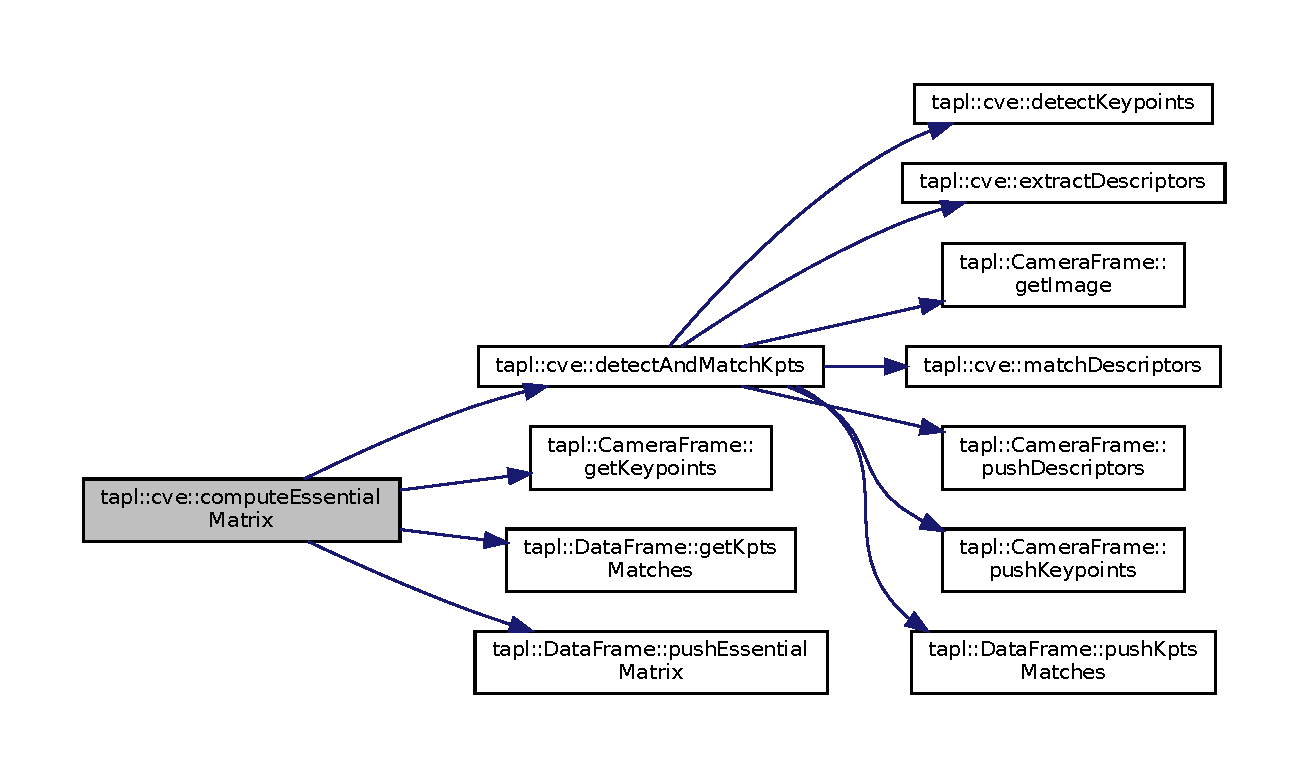
\includegraphics[width=350pt]{namespacetapl_1_1cve_a30da40f2aa0e434425c7b14f23b59457_cgraph}
\end{center}
\end{figure}
\mbox{\Hypertarget{namespacetapl_1_1cve_a8e1c9ef8d5eae6975b5e7e7c360fc1e8}\label{namespacetapl_1_1cve_a8e1c9ef8d5eae6975b5e7e7c360fc1e8}} 
\index{tapl::cve@{tapl::cve}!computeFundamentalMatrix@{computeFundamentalMatrix}}
\index{computeFundamentalMatrix@{computeFundamentalMatrix}!tapl::cve@{tapl::cve}}
\doxysubsubsection{\texorpdfstring{computeFundamentalMatrix()}{computeFundamentalMatrix()}}
{\footnotesize\ttfamily \mbox{\hyperlink{namespacetapl_a196ce1d5bf399fc26f03797e6a8d03ff}{tapl\+::\+Result\+Code}} tapl\+::cve\+::compute\+Fundamental\+Matrix (\begin{DoxyParamCaption}\item[{\mbox{\hyperlink{structtapl_1_1DataFrame}{tapl\+::\+Data\+Frame}} \&}]{dframe1,  }\item[{\mbox{\hyperlink{structtapl_1_1DataFrame}{tapl\+::\+Data\+Frame}} \&}]{dframe2 }\end{DoxyParamCaption})}



This function retrieves fundamental matrix between two images contained within their data frame structure. 


\begin{DoxyParams}[1]{Parameters}
\mbox{\texttt{ in,out}}  & {\em dframe1} & first data frame -\/ query/source/current frame \\
\hline
\mbox{\texttt{ in,out}}  & {\em dframe1} & second data frame -\/ train/reference/previous frame\\
\hline
\end{DoxyParams}
\begin{DoxyReturn}{Returns}
\mbox{\hyperlink{namespacetapl_a196ce1d5bf399fc26f03797e6a8d03ffafbdd78b1e8654e11461f37fea68c6195}{tapl\+::\+S\+U\+C\+C\+E\+SS}} if success 

\mbox{\hyperlink{namespacetapl_a196ce1d5bf399fc26f03797e6a8d03ffaa6e243674a964518a62bdda7f20f6453}{tapl\+::\+F\+A\+I\+L\+U\+RE}} if failure ~\newline

\end{DoxyReturn}
This function computes Fundamental Matrix given two image frames 

Definition at line 325 of file cv\+Engine.\+cpp.

Here is the call graph for this function\+:
\nopagebreak
\begin{figure}[H]
\begin{center}
\leavevmode
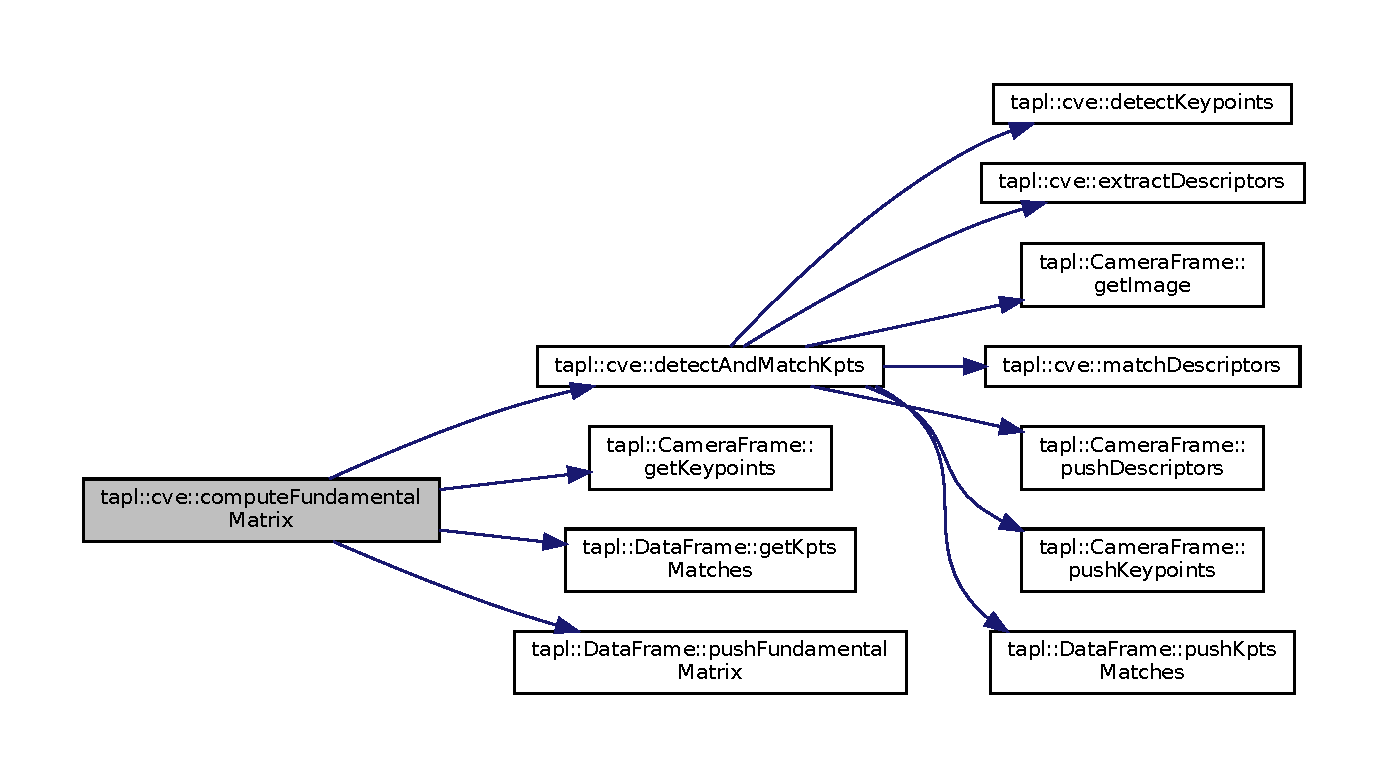
\includegraphics[width=350pt]{namespacetapl_1_1cve_a8e1c9ef8d5eae6975b5e7e7c360fc1e8_cgraph}
\end{center}
\end{figure}
\mbox{\Hypertarget{namespacetapl_1_1cve_ad8314ef8898d3a90c6d93a514bf75d20}\label{namespacetapl_1_1cve_ad8314ef8898d3a90c6d93a514bf75d20}} 
\index{tapl::cve@{tapl::cve}!computeRelativePose@{computeRelativePose}}
\index{computeRelativePose@{computeRelativePose}!tapl::cve@{tapl::cve}}
\doxysubsubsection{\texorpdfstring{computeRelativePose()}{computeRelativePose()}}
{\footnotesize\ttfamily \mbox{\hyperlink{namespacetapl_a196ce1d5bf399fc26f03797e6a8d03ff}{tapl\+::\+Result\+Code}} tapl\+::cve\+::compute\+Relative\+Pose (\begin{DoxyParamCaption}\item[{\mbox{\hyperlink{structtapl_1_1DataFrame}{tapl\+::\+Data\+Frame}} \&}]{dframe1,  }\item[{\mbox{\hyperlink{structtapl_1_1DataFrame}{tapl\+::\+Data\+Frame}} \&}]{dframe2,  }\item[{cv\+::\+Mat \&}]{camera\+\_\+matrix }\end{DoxyParamCaption})}



This function is used to compute the relative camera pose. Pose is computed for second image contained within dframe2 relative to dframe1. 


\begin{DoxyParams}[1]{Parameters}
\mbox{\texttt{ in,out}}  & {\em dframe1} & first data frame -\/ query/source/current frame \\
\hline
\mbox{\texttt{ in,out}}  & {\em dframe1} & second data frame -\/ train/reference/previous frame\\
\hline
\end{DoxyParams}
\begin{DoxyReturn}{Returns}
\mbox{\hyperlink{namespacetapl_a196ce1d5bf399fc26f03797e6a8d03ffafbdd78b1e8654e11461f37fea68c6195}{tapl\+::\+S\+U\+C\+C\+E\+SS}} if success 

\mbox{\hyperlink{namespacetapl_a196ce1d5bf399fc26f03797e6a8d03ffaa6e243674a964518a62bdda7f20f6453}{tapl\+::\+F\+A\+I\+L\+U\+RE}} if failure
\end{DoxyReturn}
This function computes relative camera pose between set of image frames 

Definition at line 427 of file cv\+Engine.\+cpp.

Here is the call graph for this function\+:
\nopagebreak
\begin{figure}[H]
\begin{center}
\leavevmode
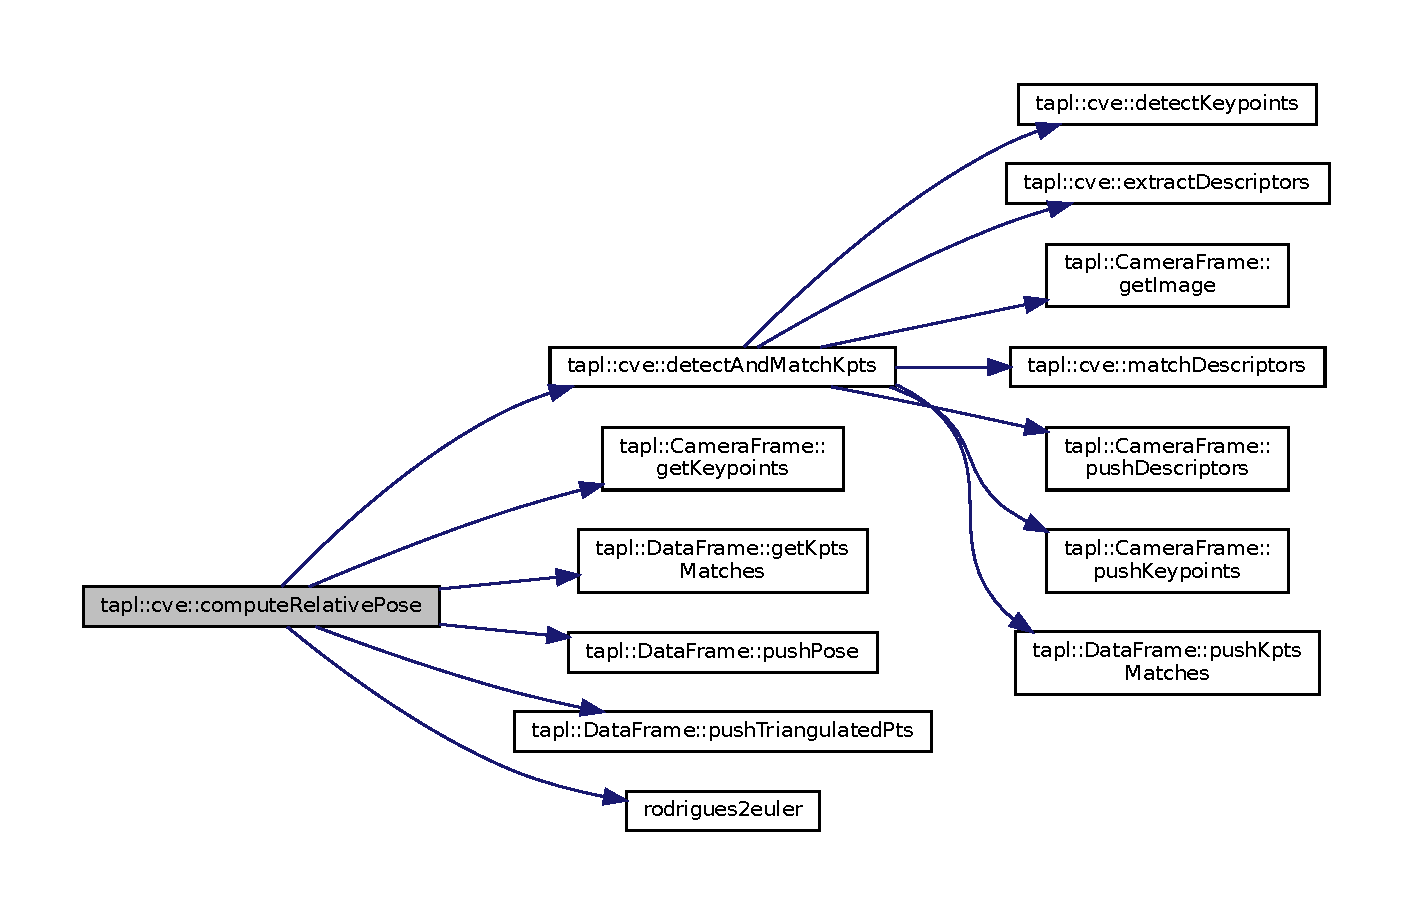
\includegraphics[width=350pt]{namespacetapl_1_1cve_ad8314ef8898d3a90c6d93a514bf75d20_cgraph}
\end{center}
\end{figure}
\mbox{\Hypertarget{namespacetapl_1_1cve_a34cb000d47a121549e81900da9913299}\label{namespacetapl_1_1cve_a34cb000d47a121549e81900da9913299}} 
\index{tapl::cve@{tapl::cve}!detectAndMatchKpts@{detectAndMatchKpts}}
\index{detectAndMatchKpts@{detectAndMatchKpts}!tapl::cve@{tapl::cve}}
\doxysubsubsection{\texorpdfstring{detectAndMatchKpts()}{detectAndMatchKpts()}}
{\footnotesize\ttfamily \mbox{\hyperlink{namespacetapl_a196ce1d5bf399fc26f03797e6a8d03ff}{tapl\+::\+Result\+Code}} tapl\+::cve\+::detect\+And\+Match\+Kpts (\begin{DoxyParamCaption}\item[{\mbox{\hyperlink{structtapl_1_1DataFrame}{tapl\+::\+Data\+Frame}} \&}]{dframe1,  }\item[{\mbox{\hyperlink{structtapl_1_1DataFrame}{tapl\+::\+Data\+Frame}} \&}]{dframe2 }\end{DoxyParamCaption})}



This function detects keypoints in two image frames and perform keypoints matching. 


\begin{DoxyParams}[1]{Parameters}
\mbox{\texttt{ in,out}}  & {\em dframe1} & first data frame -\/ query/source/current frame \\
\hline
\mbox{\texttt{ in,out}}  & {\em dframe2} & second data frame -\/ train/reference/previous frame\\
\hline
\end{DoxyParams}
\begin{DoxyReturn}{Returns}
\mbox{\hyperlink{namespacetapl_a196ce1d5bf399fc26f03797e6a8d03ffafbdd78b1e8654e11461f37fea68c6195}{tapl\+::\+S\+U\+C\+C\+E\+SS}} if success 

\mbox{\hyperlink{namespacetapl_a196ce1d5bf399fc26f03797e6a8d03ffaa6e243674a964518a62bdda7f20f6453}{tapl\+::\+F\+A\+I\+L\+U\+RE}} if failure
\end{DoxyReturn}
Detect and Match Keypoints; Store the result back into \mbox{\hyperlink{structtapl_1_1DataFrame}{tapl\+::\+Data\+Frame}} 

Definition at line 266 of file cv\+Engine.\+cpp.

Here is the call graph for this function\+:
\nopagebreak
\begin{figure}[H]
\begin{center}
\leavevmode
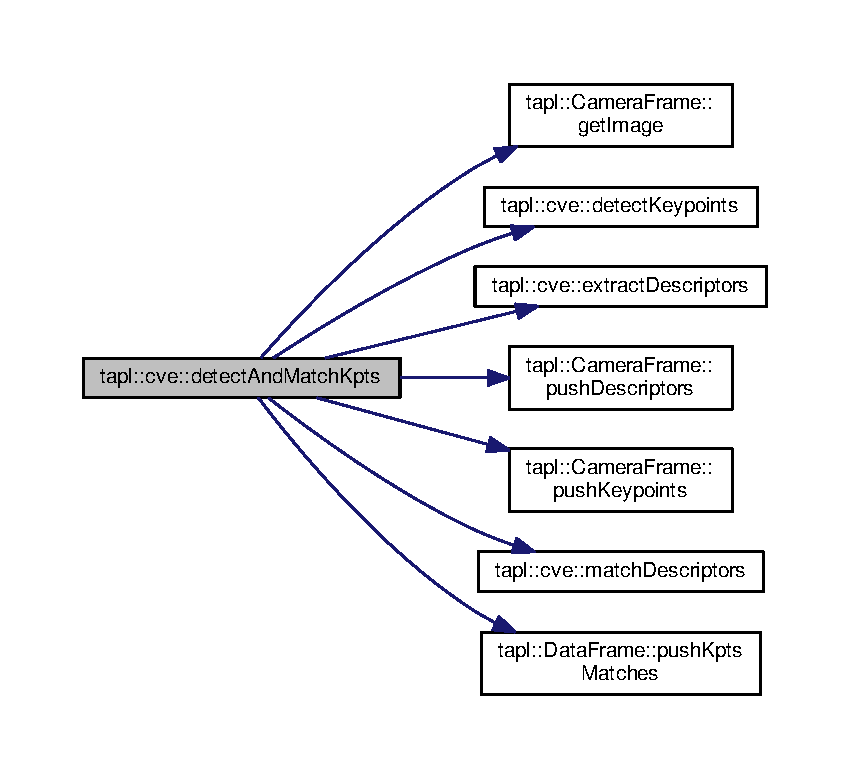
\includegraphics[width=350pt]{namespacetapl_1_1cve_a34cb000d47a121549e81900da9913299_cgraph}
\end{center}
\end{figure}
Here is the caller graph for this function\+:
\nopagebreak
\begin{figure}[H]
\begin{center}
\leavevmode
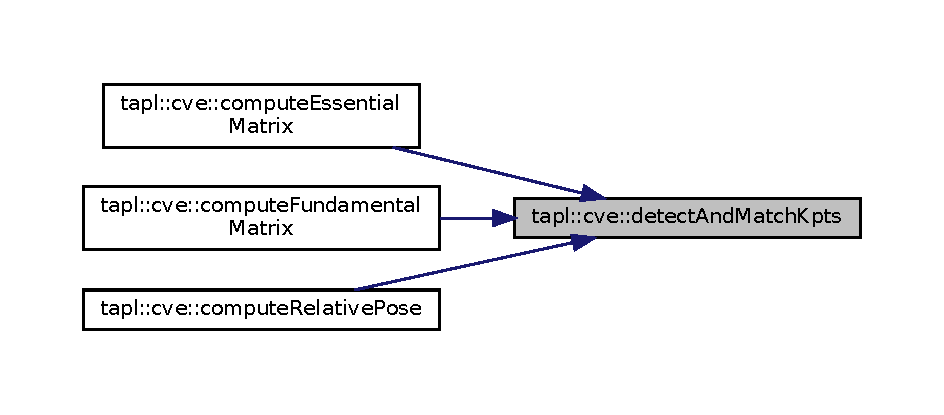
\includegraphics[width=350pt]{namespacetapl_1_1cve_a34cb000d47a121549e81900da9913299_icgraph}
\end{center}
\end{figure}
\mbox{\Hypertarget{namespacetapl_1_1cve_ad74b56dc35c6a902870725543d5df419}\label{namespacetapl_1_1cve_ad74b56dc35c6a902870725543d5df419}} 
\index{tapl::cve@{tapl::cve}!detectKeypoints@{detectKeypoints}}
\index{detectKeypoints@{detectKeypoints}!tapl::cve@{tapl::cve}}
\doxysubsubsection{\texorpdfstring{detectKeypoints()}{detectKeypoints()}}
{\footnotesize\ttfamily \mbox{\hyperlink{namespacetapl_a196ce1d5bf399fc26f03797e6a8d03ff}{tapl\+::\+Result\+Code}} tapl\+::cve\+::detect\+Keypoints (\begin{DoxyParamCaption}\item[{cv\+::\+Mat \&}]{img,  }\item[{std\+::vector$<$ cv\+::\+Key\+Point $>$ \&}]{keypoints,  }\item[{std\+::string}]{detector\+Type = {\ttfamily \char`\"{}FAST\char`\"{}} }\end{DoxyParamCaption})}



This function detects keypoints in an image. 


\begin{DoxyParams}[1]{Parameters}
\mbox{\texttt{ in}}  & {\em img} & image for which keypoints need to be detected \\
\hline
\mbox{\texttt{ out}}  & {\em keypoints} & detected keypoints \\
\hline
\mbox{\texttt{ in}}  & {\em detector\+Type} & detector types; S\+H\+I\+T\+O\+M\+A\+SI, H\+A\+R\+R\+IS, F\+A\+ST, B\+R\+I\+SK, O\+RB, A\+K\+A\+ZE, S\+I\+FT\\
\hline
\end{DoxyParams}
\begin{DoxyReturn}{Returns}
\mbox{\hyperlink{namespacetapl_a196ce1d5bf399fc26f03797e6a8d03ffafbdd78b1e8654e11461f37fea68c6195}{tapl\+::\+S\+U\+C\+C\+E\+SS}} if success 

\mbox{\hyperlink{namespacetapl_a196ce1d5bf399fc26f03797e6a8d03ffaa6e243674a964518a62bdda7f20f6453}{tapl\+::\+F\+A\+I\+L\+U\+RE}} if failure 
\end{DoxyReturn}


Definition at line 20 of file cv\+Engine.\+cpp.

Here is the caller graph for this function\+:
\nopagebreak
\begin{figure}[H]
\begin{center}
\leavevmode
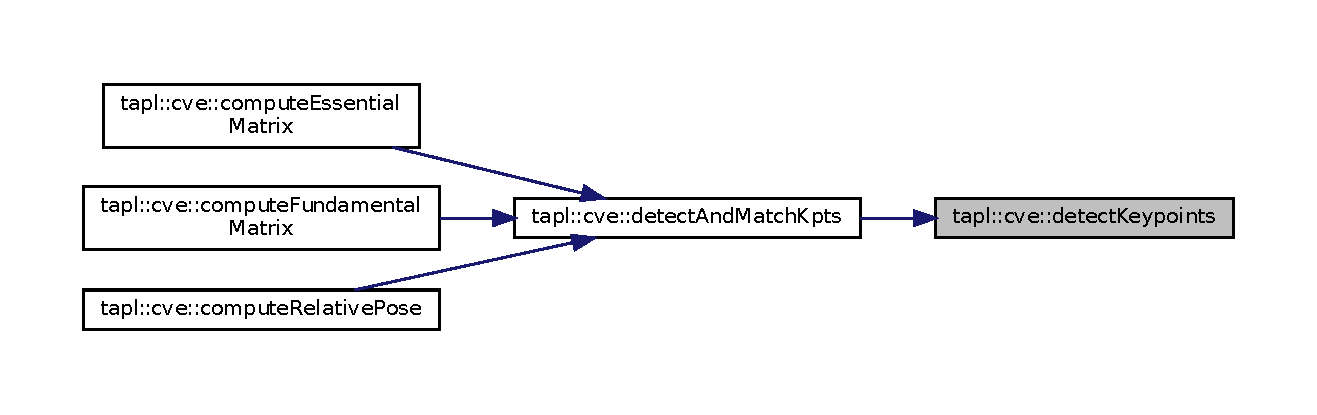
\includegraphics[width=350pt]{namespacetapl_1_1cve_ad74b56dc35c6a902870725543d5df419_icgraph}
\end{center}
\end{figure}
\mbox{\Hypertarget{namespacetapl_1_1cve_a02712316099758c2b4d0bb0e4e5dc219}\label{namespacetapl_1_1cve_a02712316099758c2b4d0bb0e4e5dc219}} 
\index{tapl::cve@{tapl::cve}!extractDescriptors@{extractDescriptors}}
\index{extractDescriptors@{extractDescriptors}!tapl::cve@{tapl::cve}}
\doxysubsubsection{\texorpdfstring{extractDescriptors()}{extractDescriptors()}}
{\footnotesize\ttfamily \mbox{\hyperlink{namespacetapl_a196ce1d5bf399fc26f03797e6a8d03ff}{tapl\+::\+Result\+Code}} tapl\+::cve\+::extract\+Descriptors (\begin{DoxyParamCaption}\item[{cv\+::\+Mat \&}]{img,  }\item[{std\+::vector$<$ cv\+::\+Key\+Point $>$ \&}]{keypoints,  }\item[{cv\+::\+Mat \&}]{descriptors,  }\item[{std\+::string}]{descriptor\+Type = {\ttfamily \char`\"{}BRISK\char`\"{}} }\end{DoxyParamCaption})}



This function extracts keypoints descriptors in an image. 


\begin{DoxyParams}[1]{Parameters}
\mbox{\texttt{ in}}  & {\em img} & image for which keypoints need to be detected \\
\hline
\mbox{\texttt{ in}}  & {\em keypoints} & keypoints \\
\hline
\mbox{\texttt{ out}}  & {\em descriptors} & output descriptors \\
\hline
\mbox{\texttt{ in}}  & {\em descriptor\+Type} & descriptor types; options\+: B\+R\+I\+SK, B\+R\+I\+EF, O\+RB, F\+R\+E\+AK, A\+K\+A\+ZE, S\+I\+FT\\
\hline
\end{DoxyParams}
\begin{DoxyReturn}{Returns}
\mbox{\hyperlink{namespacetapl_a196ce1d5bf399fc26f03797e6a8d03ffafbdd78b1e8654e11461f37fea68c6195}{tapl\+::\+S\+U\+C\+C\+E\+SS}} if success 

\mbox{\hyperlink{namespacetapl_a196ce1d5bf399fc26f03797e6a8d03ffaa6e243674a964518a62bdda7f20f6453}{tapl\+::\+F\+A\+I\+L\+U\+RE}} if failure 
\end{DoxyReturn}


Definition at line 143 of file cv\+Engine.\+cpp.

Here is the caller graph for this function\+:
\nopagebreak
\begin{figure}[H]
\begin{center}
\leavevmode
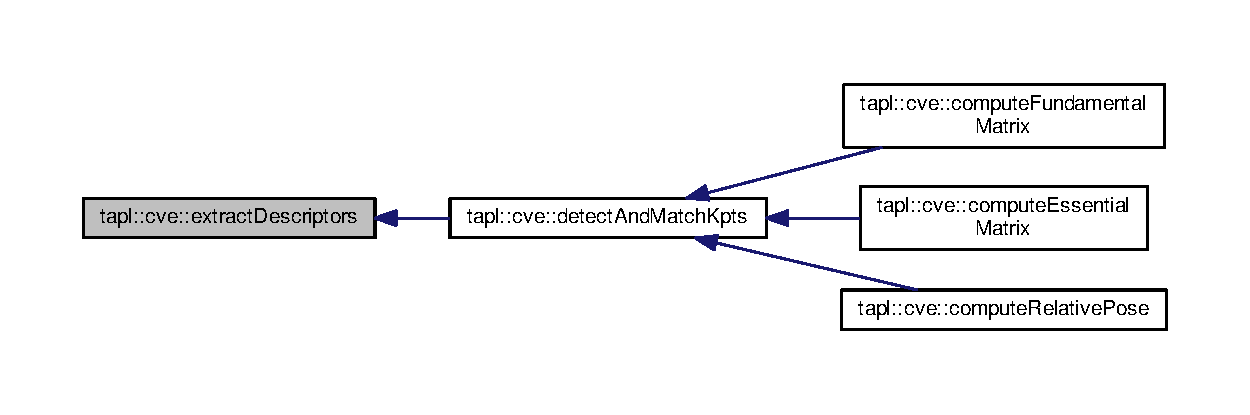
\includegraphics[width=350pt]{namespacetapl_1_1cve_a02712316099758c2b4d0bb0e4e5dc219_icgraph}
\end{center}
\end{figure}
\mbox{\Hypertarget{namespacetapl_1_1cve_ae2699cc690841efd3b7a3179be1fb889}\label{namespacetapl_1_1cve_ae2699cc690841efd3b7a3179be1fb889}} 
\index{tapl::cve@{tapl::cve}!matchDescriptors@{matchDescriptors}}
\index{matchDescriptors@{matchDescriptors}!tapl::cve@{tapl::cve}}
\doxysubsubsection{\texorpdfstring{matchDescriptors()}{matchDescriptors()}}
{\footnotesize\ttfamily \mbox{\hyperlink{namespacetapl_a196ce1d5bf399fc26f03797e6a8d03ff}{tapl\+::\+Result\+Code}} tapl\+::cve\+::match\+Descriptors (\begin{DoxyParamCaption}\item[{std\+::vector$<$ cv\+::\+Key\+Point $>$ \&}]{k\+Pts\+Source,  }\item[{std\+::vector$<$ cv\+::\+Key\+Point $>$ \&}]{k\+Pts\+Ref,  }\item[{cv\+::\+Mat \&}]{desc\+Source,  }\item[{cv\+::\+Mat \&}]{desc\+Ref,  }\item[{std\+::vector$<$ cv\+::\+D\+Match $>$ \&}]{matches,  }\item[{std\+::string}]{norm\+Type = {\ttfamily \char`\"{}NORM\+\_\+HAMMING\char`\"{}},  }\item[{std\+::string}]{matcher\+Type = {\ttfamily \char`\"{}MAT\+\_\+BF\char`\"{}},  }\item[{std\+::string}]{selector\+Type = {\ttfamily \char`\"{}SEL\+\_\+KNN\char`\"{}} }\end{DoxyParamCaption})}



This function performs keypoint descriptor matching. 


\begin{DoxyParams}[1]{Parameters}
\mbox{\texttt{ in}}  & {\em k\+Pts\+Source} & keypoints in the source/query image \\
\hline
\mbox{\texttt{ in}}  & {\em k\+Pts\+Ref} & keypoints in the reference/train image \\
\hline
\mbox{\texttt{ in}}  & {\em desc\+Source} & descriptors in the source/query image \\
\hline
\mbox{\texttt{ in}}  & {\em desc\+Ref} & descriptors in the reference/train image \\
\hline
\mbox{\texttt{ out}}  & {\em matches} & descriptor match output \\
\hline
\mbox{\texttt{ in}}  & {\em norm\+Type} & norm types; options\+: N\+O\+R\+M\+\_\+\+H\+A\+M\+M\+I\+NG, N\+O\+R\+M\+\_\+\+L2 N\+O\+R\+M\+\_\+\+H\+A\+M\+M\+I\+NG \+: Hamming Distance L2\+\_\+\+H\+A\+M\+M\+I\+NG \+: L2 Distance \\
\hline
\mbox{\texttt{ in}}  & {\em matcher\+Type} & types; options\+: M\+A\+T\+\_\+\+BF, M\+A\+T\+\_\+\+F\+L\+A\+NN M\+A\+T\+\_\+\+BF \+: Brute-\/\+Force Matching M\+A\+T\+\_\+\+F\+L\+A\+NN \+: F\+L\+A\+NN based matching ~\newline
 \\
\hline
\mbox{\texttt{ in}}  & {\em selector\+Type} & types; options\+: S\+E\+L\+\_\+\+NN, S\+E\+L\+\_\+\+K\+NN S\+E\+L\+\_\+\+NN \+: Nearest-\/\+Neighbor S\+E\+L\+\_\+\+K\+NN \+: K-\/\+Nearest-\/\+Neighbor\\
\hline
\end{DoxyParams}
\begin{DoxyReturn}{Returns}
\mbox{\hyperlink{namespacetapl_a196ce1d5bf399fc26f03797e6a8d03ffafbdd78b1e8654e11461f37fea68c6195}{tapl\+::\+S\+U\+C\+C\+E\+SS}} if success 

\mbox{\hyperlink{namespacetapl_a196ce1d5bf399fc26f03797e6a8d03ffaa6e243674a964518a62bdda7f20f6453}{tapl\+::\+F\+A\+I\+L\+U\+RE}} if failure 
\end{DoxyReturn}


Definition at line 197 of file cv\+Engine.\+cpp.

Here is the caller graph for this function\+:
\nopagebreak
\begin{figure}[H]
\begin{center}
\leavevmode
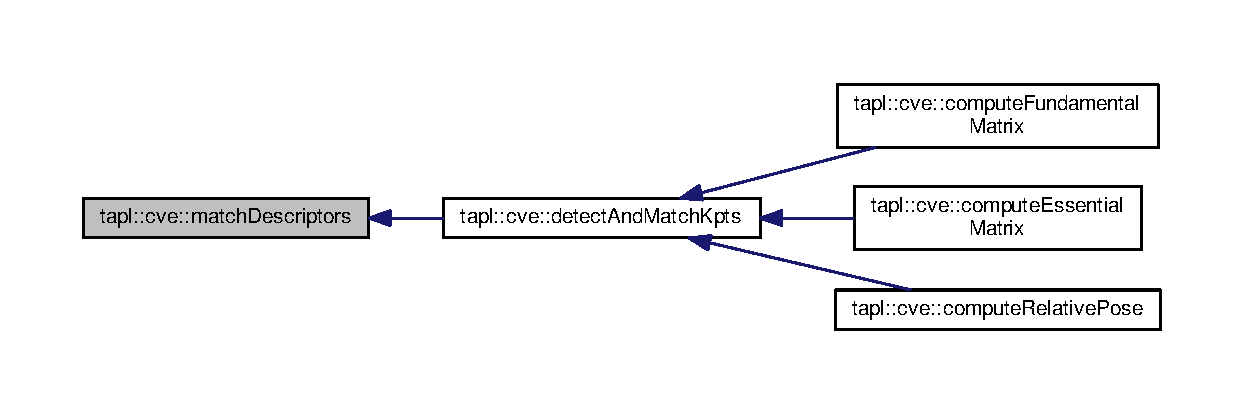
\includegraphics[width=350pt]{namespacetapl_1_1cve_ae2699cc690841efd3b7a3179be1fb889_icgraph}
\end{center}
\end{figure}
\mbox{\Hypertarget{namespacetapl_1_1cve_aab4041f410589ff960febecf36b3ee2b}\label{namespacetapl_1_1cve_aab4041f410589ff960febecf36b3ee2b}} 
\index{tapl::cve@{tapl::cve}!stitchPanaromic@{stitchPanaromic}}
\index{stitchPanaromic@{stitchPanaromic}!tapl::cve@{tapl::cve}}
\doxysubsubsection{\texorpdfstring{stitchPanaromic()}{stitchPanaromic()}}
{\footnotesize\ttfamily \mbox{\hyperlink{namespacetapl_a196ce1d5bf399fc26f03797e6a8d03ff}{tapl\+::\+Result\+Code}} tapl\+::cve\+::stitch\+Panaromic (\begin{DoxyParamCaption}\item[{const std\+::vector$<$ cv\+::\+Mat $>$ \&}]{imgs,  }\item[{cv\+::\+Mat \&}]{panoramic\+\_\+img }\end{DoxyParamCaption})}



This function is used to stitch multiple images as a panaromic image. 


\begin{DoxyParams}[1]{Parameters}
\mbox{\texttt{ in}}  & {\em imgs} & list of images \\
\hline
\mbox{\texttt{ out}}  & {\em panoramic\+\_\+img} & stitched panoramic image\\
\hline
\end{DoxyParams}
\begin{DoxyReturn}{Returns}
\mbox{\hyperlink{namespacetapl_a196ce1d5bf399fc26f03797e6a8d03ffafbdd78b1e8654e11461f37fea68c6195}{tapl\+::\+S\+U\+C\+C\+E\+SS}} if success 

\mbox{\hyperlink{namespacetapl_a196ce1d5bf399fc26f03797e6a8d03ffaa6e243674a964518a62bdda7f20f6453}{tapl\+::\+F\+A\+I\+L\+U\+RE}} if failure 
\end{DoxyReturn}


Definition at line 511 of file cv\+Engine.\+cpp.


\hypertarget{namespacetapl_1_1pte}{}\doxysection{tapl\+::pte Namespace Reference}
\label{namespacetapl_1_1pte}\index{tapl::pte@{tapl::pte}}
\doxysubsection*{Data Structures}
\begin{DoxyCompactItemize}
\item 
class \mbox{\hyperlink{classtapl_1_1pte_1_1EuclideanCluster}{Euclidean\+Cluster}}
\item 
struct \mbox{\hyperlink{structtapl_1_1pte_1_1KdTree}{Kd\+Tree}}
\item 
class \mbox{\hyperlink{classtapl_1_1pte_1_1Line}{Line}}
\item 
struct \mbox{\hyperlink{structtapl_1_1pte_1_1Node}{Node}}
\item 
class \mbox{\hyperlink{classtapl_1_1pte_1_1Plane}{Plane}}
\end{DoxyCompactItemize}
\doxysubsection*{Functions}
\begin{DoxyCompactItemize}
\item 
cv\+::\+Mat \mbox{\hyperlink{namespacetapl_1_1pte_a874efe99ea9c6366ae0c0329554ad200}{world2\+Cam\+Rotation}} ()
\begin{DoxyCompactList}\small\item\em returns world to camera rotation matrix \end{DoxyCompactList}\item 
{\footnotesize template$<$typename PointT $>$ }\\void \mbox{\hyperlink{namespacetapl_1_1pte_a928126360beb48c632ff331ca560a1b0}{world2\+Cam\+Coordinate}} (PointT \&point)
\begin{DoxyCompactList}\small\item\em affine transform on a point \end{DoxyCompactList}\item 
{\footnotesize template$<$typename PointT $>$ }\\void \mbox{\hyperlink{namespacetapl_1_1pte_a48c0b0806659501276e0b33042e2fa5b}{downsample\+Cloud}} (typename pcl\+::\+Point\+Cloud$<$ PointT $>$\+::Ptr cloud, float resolution)
\begin{DoxyCompactList}\small\item\em Downsample point-\/cloud. \end{DoxyCompactList}\item 
{\footnotesize template$<$typename PointT $>$ }\\void \mbox{\hyperlink{namespacetapl_1_1pte_adaa36d31de7cd145e875901dfa13a616}{crop\+Cloud}} (typename pcl\+::\+Point\+Cloud$<$ PointT $>$\+::Ptr cloud, float x\+\_\+min, float x\+\_\+max, float y\+\_\+min, float y\+\_\+max, float z\+\_\+min, float z\+\_\+max)
\begin{DoxyCompactList}\small\item\em Crop point-\/cloud given a region of interest. \end{DoxyCompactList}\item 
{\footnotesize template$<$typename PointT $>$ }\\\mbox{\hyperlink{namespacetapl_a196ce1d5bf399fc26f03797e6a8d03ff}{tapl\+::\+Result\+Code}} \mbox{\hyperlink{namespacetapl_1_1pte_aa4fc09affe62218081e85ed5818bf2ef}{segment\+Plane}} (typename pcl\+::\+Point\+Cloud$<$ PointT $>$\+::Ptr cloud, std\+::pair$<$ typename pcl\+::\+Point\+Cloud$<$ PointT $>$\+::Ptr, typename pcl\+::\+Point\+Cloud$<$ PointT $>$\+::Ptr $>$ \&seg\+Result, int max\+Iterations, float distance\+Threshold, bool use\+P\+CL=false)
\begin{DoxyCompactList}\small\item\em This function segments a plane within a point-\/cloud. Points within the plane are inliers and other points are outliers. It populates two separate point-\/clouds corresponding to inliers and outliers. \end{DoxyCompactList}\item 
{\footnotesize template$<$typename PointT $>$ }\\std\+::vector$<$ typename pcl\+::\+Point\+Cloud$<$ PointT $>$\+::Ptr $>$ \mbox{\hyperlink{namespacetapl_1_1pte_a69e06eaa64248177550033adb709fb3d}{euclidean\+Clustering}} (typename pcl\+::\+Point\+Cloud$<$ PointT $>$\+::Ptr cloud, float cluster\+Tolerance, int min\+Num\+Points, int max\+Num\+Points, bool use\+P\+CL=false)
\begin{DoxyCompactList}\small\item\em Perform euclidean clustering within a point-\/cloud. Returns a vector of cluster clouds. \end{DoxyCompactList}\item 
{\footnotesize template$<$typename PointT $>$ }\\\mbox{\hyperlink{structtapl_1_1BBox3d}{tapl\+::\+B\+Box3d}} \mbox{\hyperlink{namespacetapl_1_1pte_ac4b4a53485d62466140d43448496536b}{get\+Bounding\+Box}} (typename pcl\+::\+Point\+Cloud$<$ PointT $>$\+::Ptr cloud\+Cluster)
\begin{DoxyCompactList}\small\item\em This function is used to obtain bounding-\/box for a cluster of points. \end{DoxyCompactList}\end{DoxyCompactItemize}


\doxysubsection{Function Documentation}
\mbox{\Hypertarget{namespacetapl_1_1pte_adaa36d31de7cd145e875901dfa13a616}\label{namespacetapl_1_1pte_adaa36d31de7cd145e875901dfa13a616}} 
\index{tapl::pte@{tapl::pte}!cropCloud@{cropCloud}}
\index{cropCloud@{cropCloud}!tapl::pte@{tapl::pte}}
\doxysubsubsection{\texorpdfstring{cropCloud()}{cropCloud()}}
{\footnotesize\ttfamily template$<$typename PointT $>$ \\
void tapl\+::pte\+::crop\+Cloud (\begin{DoxyParamCaption}\item[{typename pcl\+::\+Point\+Cloud$<$ PointT $>$\+::Ptr}]{cloud,  }\item[{float}]{x\+\_\+min,  }\item[{float}]{x\+\_\+max,  }\item[{float}]{y\+\_\+min,  }\item[{float}]{y\+\_\+max,  }\item[{float}]{z\+\_\+min,  }\item[{float}]{z\+\_\+max }\end{DoxyParamCaption})}



Crop point-\/cloud given a region of interest. 


\begin{DoxyParams}[1]{Parameters}
\mbox{\texttt{ in,out}}  & {\em cloud} & Point-\/\+Cloud \\
\hline
\mbox{\texttt{ in}}  & {\em x\+\_\+min} & minimum point x-\/coordinate \\
\hline
\mbox{\texttt{ in}}  & {\em x\+\_\+max} & maximum point x-\/coordinate \\
\hline
\mbox{\texttt{ in}}  & {\em y\+\_\+min} & minimum point y-\/coordinate \\
\hline
\mbox{\texttt{ in}}  & {\em y\+\_\+max} & maximum point y-\/coordinate \\
\hline
\mbox{\texttt{ in}}  & {\em z\+\_\+min} & minimum point z-\/coordinate \\
\hline
\mbox{\texttt{ in}}  & {\em z\+\_\+max} & maximum point z-\/coordinate \\
\hline
\end{DoxyParams}


Definition at line 253 of file pt\+Engine.\+hpp.

\mbox{\Hypertarget{namespacetapl_1_1pte_a48c0b0806659501276e0b33042e2fa5b}\label{namespacetapl_1_1pte_a48c0b0806659501276e0b33042e2fa5b}} 
\index{tapl::pte@{tapl::pte}!downsampleCloud@{downsampleCloud}}
\index{downsampleCloud@{downsampleCloud}!tapl::pte@{tapl::pte}}
\doxysubsubsection{\texorpdfstring{downsampleCloud()}{downsampleCloud()}}
{\footnotesize\ttfamily template$<$typename PointT $>$ \\
void tapl\+::pte\+::downsample\+Cloud (\begin{DoxyParamCaption}\item[{typename pcl\+::\+Point\+Cloud$<$ PointT $>$\+::Ptr}]{cloud,  }\item[{float}]{resolution }\end{DoxyParamCaption})}



Downsample point-\/cloud. 


\begin{DoxyParams}[1]{Parameters}
\mbox{\texttt{ in,out}}  & {\em cloud} & Point-\/\+Cloud \\
\hline
\mbox{\texttt{ in}}  & {\em resolution} & Target resolution for downsampling the cloud \\
\hline
\end{DoxyParams}


Definition at line 232 of file pt\+Engine.\+hpp.

\mbox{\Hypertarget{namespacetapl_1_1pte_a69e06eaa64248177550033adb709fb3d}\label{namespacetapl_1_1pte_a69e06eaa64248177550033adb709fb3d}} 
\index{tapl::pte@{tapl::pte}!euclideanClustering@{euclideanClustering}}
\index{euclideanClustering@{euclideanClustering}!tapl::pte@{tapl::pte}}
\doxysubsubsection{\texorpdfstring{euclideanClustering()}{euclideanClustering()}}
{\footnotesize\ttfamily template$<$typename PointT $>$ \\
std\+::vector$<$typename pcl\+::\+Point\+Cloud$<$PointT$>$\+::Ptr$>$ tapl\+::pte\+::euclidean\+Clustering (\begin{DoxyParamCaption}\item[{typename pcl\+::\+Point\+Cloud$<$ PointT $>$\+::Ptr}]{cloud,  }\item[{float}]{cluster\+Tolerance,  }\item[{int}]{min\+Num\+Points,  }\item[{int}]{max\+Num\+Points,  }\item[{bool}]{use\+P\+CL = {\ttfamily false} }\end{DoxyParamCaption})}



Perform euclidean clustering within a point-\/cloud. Returns a vector of cluster clouds. 


\begin{DoxyParams}[1]{Parameters}
\mbox{\texttt{ in}}  & {\em cloud} & point-\/cloud to segment \\
\hline
\mbox{\texttt{ in}}  & {\em cluster\+Tolerance} & distance tolerance for considering a point as part of the cluster. \\
\hline
\mbox{\texttt{ in}}  & {\em min\+Num\+Points} & minimum number of points in a neighborhood to be considered as a cluster \\
\hline
\mbox{\texttt{ in}}  & {\em max\+Num\+Points} & maximum number of points in a neighborhood to be considered as a cluster \\
\hline
\mbox{\texttt{ in}}  & {\em use\+P\+CL} & Whether to use P\+CL of T\+A\+PL\textquotesingle{}s implementation of R\+A\+N\+S\+AC\\
\hline
\end{DoxyParams}
\begin{DoxyReturn}{Returns}
Vector of cluster point-\/clouds 
\end{DoxyReturn}


Definition at line 375 of file pt\+Engine.\+hpp.

Here is the call graph for this function\+:
\nopagebreak
\begin{figure}[H]
\begin{center}
\leavevmode
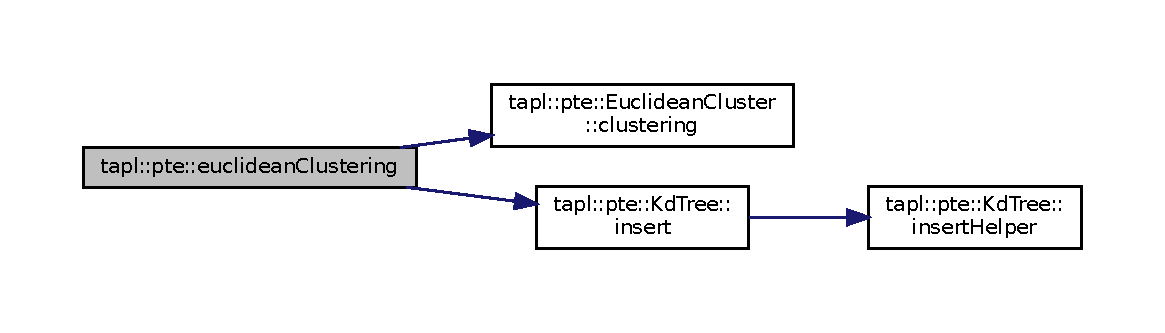
\includegraphics[width=350pt]{namespacetapl_1_1pte_a69e06eaa64248177550033adb709fb3d_cgraph}
\end{center}
\end{figure}
\mbox{\Hypertarget{namespacetapl_1_1pte_ac4b4a53485d62466140d43448496536b}\label{namespacetapl_1_1pte_ac4b4a53485d62466140d43448496536b}} 
\index{tapl::pte@{tapl::pte}!getBoundingBox@{getBoundingBox}}
\index{getBoundingBox@{getBoundingBox}!tapl::pte@{tapl::pte}}
\doxysubsubsection{\texorpdfstring{getBoundingBox()}{getBoundingBox()}}
{\footnotesize\ttfamily template$<$typename PointT $>$ \\
\mbox{\hyperlink{structtapl_1_1BBox3d}{tapl\+::\+B\+Box3d}} tapl\+::pte\+::get\+Bounding\+Box (\begin{DoxyParamCaption}\item[{typename pcl\+::\+Point\+Cloud$<$ PointT $>$\+::Ptr}]{cloud\+Cluster }\end{DoxyParamCaption})}



This function is used to obtain bounding-\/box for a cluster of points. 


\begin{DoxyParams}[1]{Parameters}
\mbox{\texttt{ in}}  & {\em cloud\+Cluster} & a cluster of point-\/cloud\\
\hline
\end{DoxyParams}
\begin{DoxyReturn}{Returns}
3D Bounding-\/\+Box 
\end{DoxyReturn}


Definition at line 464 of file pt\+Engine.\+hpp.

\mbox{\Hypertarget{namespacetapl_1_1pte_aa4fc09affe62218081e85ed5818bf2ef}\label{namespacetapl_1_1pte_aa4fc09affe62218081e85ed5818bf2ef}} 
\index{tapl::pte@{tapl::pte}!segmentPlane@{segmentPlane}}
\index{segmentPlane@{segmentPlane}!tapl::pte@{tapl::pte}}
\doxysubsubsection{\texorpdfstring{segmentPlane()}{segmentPlane()}}
{\footnotesize\ttfamily template$<$typename PointT $>$ \\
\mbox{\hyperlink{namespacetapl_a196ce1d5bf399fc26f03797e6a8d03ff}{tapl\+::\+Result\+Code}} tapl\+::pte\+::segment\+Plane (\begin{DoxyParamCaption}\item[{typename pcl\+::\+Point\+Cloud$<$ PointT $>$\+::Ptr}]{cloud,  }\item[{std\+::pair$<$ typename pcl\+::\+Point\+Cloud$<$ PointT $>$\+::Ptr, typename pcl\+::\+Point\+Cloud$<$ PointT $>$\+::Ptr $>$ \&}]{seg\+Result,  }\item[{int}]{max\+Iterations,  }\item[{float}]{distance\+Threshold,  }\item[{bool}]{use\+P\+CL = {\ttfamily false} }\end{DoxyParamCaption})}



This function segments a plane within a point-\/cloud. Points within the plane are inliers and other points are outliers. It populates two separate point-\/clouds corresponding to inliers and outliers. 


\begin{DoxyParams}[1]{Parameters}
\mbox{\texttt{ in}}  & {\em cloud} & point-\/cloud to segment \\
\hline
\mbox{\texttt{ out}}  & {\em seg\+Result} & segmentation result Inliers\+: seg\+Result.\+first Outliers\+: seg\+Result.\+second \\
\hline
\mbox{\texttt{ in}}  & {\em max\+Iteration} & Maximum number of iterations for plane fitting with R\+A\+N\+S\+AC \\
\hline
\mbox{\texttt{ in}}  & {\em distance\+Threshold} & Distance threshold between point and plane for classifying a point as an inlier. \\
\hline
\mbox{\texttt{ in}}  & {\em use\+P\+CL} & Whether to use P\+CL of T\+A\+PL\textquotesingle{}s implementation of R\+A\+N\+S\+AC\\
\hline
\end{DoxyParams}
\begin{DoxyReturn}{Returns}
\mbox{\hyperlink{namespacetapl_a196ce1d5bf399fc26f03797e6a8d03ffafbdd78b1e8654e11461f37fea68c6195}{tapl\+::\+S\+U\+C\+C\+E\+SS}} if success 

\mbox{\hyperlink{namespacetapl_a196ce1d5bf399fc26f03797e6a8d03ffaa6e243674a964518a62bdda7f20f6453}{tapl\+::\+F\+A\+I\+L\+U\+RE}} if failure 
\end{DoxyReturn}


Definition at line 288 of file pt\+Engine.\+hpp.

Here is the call graph for this function\+:
\nopagebreak
\begin{figure}[H]
\begin{center}
\leavevmode
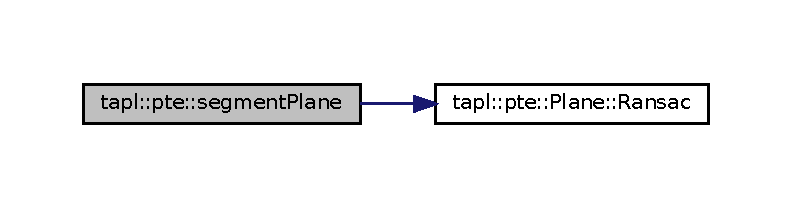
\includegraphics[width=350pt]{namespacetapl_1_1pte_aa4fc09affe62218081e85ed5818bf2ef_cgraph}
\end{center}
\end{figure}
\mbox{\Hypertarget{namespacetapl_1_1pte_a928126360beb48c632ff331ca560a1b0}\label{namespacetapl_1_1pte_a928126360beb48c632ff331ca560a1b0}} 
\index{tapl::pte@{tapl::pte}!world2CamCoordinate@{world2CamCoordinate}}
\index{world2CamCoordinate@{world2CamCoordinate}!tapl::pte@{tapl::pte}}
\doxysubsubsection{\texorpdfstring{world2CamCoordinate()}{world2CamCoordinate()}}
{\footnotesize\ttfamily template$<$typename PointT $>$ \\
void tapl\+::pte\+::world2\+Cam\+Coordinate (\begin{DoxyParamCaption}\item[{PointT \&}]{point }\end{DoxyParamCaption})}



affine transform on a point 

Apply affine transforms on point given in world coordinate

Camera Coordinate System\+: X -\/$>$ To the right Y -\/$>$ Down Z -\/$>$ Forward -\/ Direction where the camera is pointing

World Coordinate System\+: X -\/$>$ Forward -\/ Direction where the camera is pointing Y -\/$>$ To the left Z -\/$>$ Up


\begin{DoxyParams}[1]{Parameters}
\mbox{\texttt{ in}}  & {\em point} & point in world coordinate\\
\hline
\end{DoxyParams}
\begin{DoxyReturn}{Returns}
point in camera coordinate 
\end{DoxyReturn}


Definition at line 207 of file pt\+Engine.\+hpp.

Here is the call graph for this function\+:
\nopagebreak
\begin{figure}[H]
\begin{center}
\leavevmode
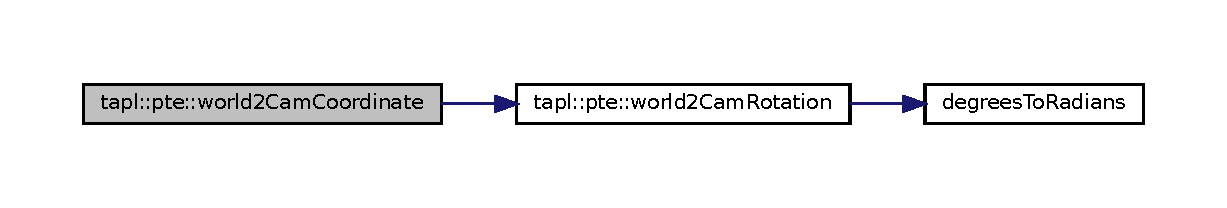
\includegraphics[width=350pt]{namespacetapl_1_1pte_a928126360beb48c632ff331ca560a1b0_cgraph}
\end{center}
\end{figure}
\mbox{\Hypertarget{namespacetapl_1_1pte_a874efe99ea9c6366ae0c0329554ad200}\label{namespacetapl_1_1pte_a874efe99ea9c6366ae0c0329554ad200}} 
\index{tapl::pte@{tapl::pte}!world2CamRotation@{world2CamRotation}}
\index{world2CamRotation@{world2CamRotation}!tapl::pte@{tapl::pte}}
\doxysubsubsection{\texorpdfstring{world2CamRotation()}{world2CamRotation()}}
{\footnotesize\ttfamily cv\+::\+Mat tapl\+::pte\+::world2\+Cam\+Rotation (\begin{DoxyParamCaption}{ }\end{DoxyParamCaption})}



returns world to camera rotation matrix 

Camera Coordinate System\+: X -\/$>$ To the right Y -\/$>$ Down Z -\/$>$ Forward -\/ Direction where the camera is pointing

World Coordinate System\+: X -\/$>$ Forward -\/ Direction where the camera is pointing Y -\/$>$ To the left Z -\/$>$ Up \begin{DoxyReturn}{Returns}
rotation matrix 
\end{DoxyReturn}


Definition at line 150 of file pt\+Engine.\+hpp.

Here is the call graph for this function\+:
\nopagebreak
\begin{figure}[H]
\begin{center}
\leavevmode
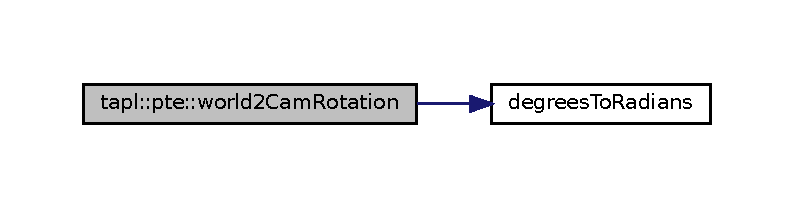
\includegraphics[width=350pt]{namespacetapl_1_1pte_a874efe99ea9c6366ae0c0329554ad200_cgraph}
\end{center}
\end{figure}
Here is the caller graph for this function\+:
\nopagebreak
\begin{figure}[H]
\begin{center}
\leavevmode
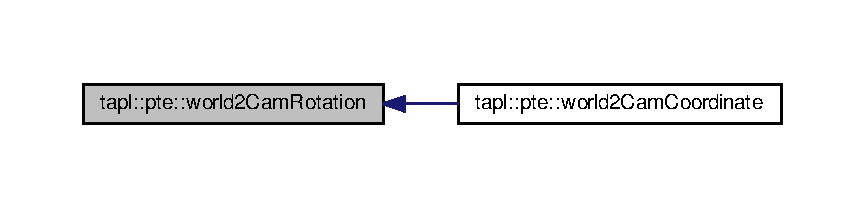
\includegraphics[width=350pt]{namespacetapl_1_1pte_a874efe99ea9c6366ae0c0329554ad200_icgraph}
\end{center}
\end{figure}

\hypertarget{namespacetapl_1_1viz}{}\section{tapl\+:\+:viz Namespace Reference}
\label{namespacetapl_1_1viz}\index{tapl\+::viz@{tapl\+::viz}}
\subsection*{Data Structures}
\begin{DoxyCompactItemize}
\item 
class \hyperlink{classtapl_1_1viz_1_1Visualizer}{Visualizer}
\begin{DoxyCompactList}\small\item\em Implementation of the visualizer class. \end{DoxyCompactList}\end{DoxyCompactItemize}
\subsection*{Enumerations}
\begin{DoxyCompactItemize}
\item 
enum \hyperlink{namespacetapl_1_1viz_a99e496921984514dbc7bcef809f50150}{Camera\+Angle} \{ \hyperlink{namespacetapl_1_1viz_a99e496921984514dbc7bcef809f50150a361bb774c1715ed6be67552bd2aac36e}{XY}, 
\hyperlink{namespacetapl_1_1viz_a99e496921984514dbc7bcef809f50150a9aa35eea1fe8f4b45a0b02a8b5048cfa}{Top\+Down}, 
\hyperlink{namespacetapl_1_1viz_a99e496921984514dbc7bcef809f50150aa268beeef2cb7c134c70cc8fc05b7045}{Side}, 
\hyperlink{namespacetapl_1_1viz_a99e496921984514dbc7bcef809f50150a85d72fbe54240f98c1ed1ccd5fe8b7d9}{F\+PS}
 \}\begin{DoxyCompactList}\small\item\em Enumerations for camera view angle. \end{DoxyCompactList}
\end{DoxyCompactItemize}


\subsection{Enumeration Type Documentation}
\index{tapl\+::viz@{tapl\+::viz}!Camera\+Angle@{Camera\+Angle}}
\index{Camera\+Angle@{Camera\+Angle}!tapl\+::viz@{tapl\+::viz}}
\subsubsection[{\texorpdfstring{Camera\+Angle}{CameraAngle}}]{\setlength{\rightskip}{0pt plus 5cm}enum {\bf tapl\+::viz\+::\+Camera\+Angle}}\hypertarget{namespacetapl_1_1viz_a99e496921984514dbc7bcef809f50150}{}\label{namespacetapl_1_1viz_a99e496921984514dbc7bcef809f50150}


Enumerations for camera view angle. 

\begin{Desc}
\item[Enumerator]\par
\begin{description}
\index{XY@{XY}!tapl\+::viz@{tapl\+::viz}}\index{tapl\+::viz@{tapl\+::viz}!XY@{XY}}\item[{\em 
XY\hypertarget{namespacetapl_1_1viz_a99e496921984514dbc7bcef809f50150a361bb774c1715ed6be67552bd2aac36e}{}\label{namespacetapl_1_1viz_a99e496921984514dbc7bcef809f50150a361bb774c1715ed6be67552bd2aac36e}
}]Angled XY Camera Position \index{Top\+Down@{Top\+Down}!tapl\+::viz@{tapl\+::viz}}\index{tapl\+::viz@{tapl\+::viz}!Top\+Down@{Top\+Down}}\item[{\em 
Top\+Down\hypertarget{namespacetapl_1_1viz_a99e496921984514dbc7bcef809f50150a9aa35eea1fe8f4b45a0b02a8b5048cfa}{}\label{namespacetapl_1_1viz_a99e496921984514dbc7bcef809f50150a9aa35eea1fe8f4b45a0b02a8b5048cfa}
}]Top Down View \index{Side@{Side}!tapl\+::viz@{tapl\+::viz}}\index{tapl\+::viz@{tapl\+::viz}!Side@{Side}}\item[{\em 
Side\hypertarget{namespacetapl_1_1viz_a99e496921984514dbc7bcef809f50150aa268beeef2cb7c134c70cc8fc05b7045}{}\label{namespacetapl_1_1viz_a99e496921984514dbc7bcef809f50150aa268beeef2cb7c134c70cc8fc05b7045}
}]Side View \index{F\+PS@{F\+PS}!tapl\+::viz@{tapl\+::viz}}\index{tapl\+::viz@{tapl\+::viz}!F\+PS@{F\+PS}}\item[{\em 
F\+PS\hypertarget{namespacetapl_1_1viz_a99e496921984514dbc7bcef809f50150a85d72fbe54240f98c1ed1ccd5fe8b7d9}{}\label{namespacetapl_1_1viz_a99e496921984514dbc7bcef809f50150a85d72fbe54240f98c1ed1ccd5fe8b7d9}
}]First Person View \end{description}
\end{Desc}


Definition at line 17 of file visualization.\+hpp.


\chapter{Data Structure Documentation}
\hypertarget{structtapl_1_1BBox3d}{}\doxysection{tapl\+::B\+Box3d Struct Reference}
\label{structtapl_1_1BBox3d}\index{tapl::BBox3d@{tapl::BBox3d}}


3D Bounding-\/\+Box  




{\ttfamily \#include $<$tapl\+Types.\+hpp$>$}

\doxysubsection*{Data Fields}
\begin{DoxyCompactItemize}
\item 
double \mbox{\hyperlink{structtapl_1_1BBox3d_a7f28356e5e1f7503770b352c457d4aed}{x\+\_\+min}}
\item 
double \mbox{\hyperlink{structtapl_1_1BBox3d_ae7fd61bfb33a3c5fbc7b531960d7e543}{x\+\_\+max}}
\item 
double \mbox{\hyperlink{structtapl_1_1BBox3d_a63dd683fccb905aa43e3d363c0829581}{y\+\_\+min}}
\item 
double \mbox{\hyperlink{structtapl_1_1BBox3d_ade66b3bf2e0dcf01b790d560826b64e1}{y\+\_\+max}}
\item 
double \mbox{\hyperlink{structtapl_1_1BBox3d_a62b2d92bf15298ad86a7159aadd232ab}{z\+\_\+min}}
\item 
double \mbox{\hyperlink{structtapl_1_1BBox3d_a6b1ff639ba484bdcf6185d53870d623f}{z\+\_\+max}}
\end{DoxyCompactItemize}


\doxysubsection{Detailed Description}
3D Bounding-\/\+Box 

Definition at line 36 of file tapl\+Types.\+hpp.



\doxysubsection{Field Documentation}
\mbox{\Hypertarget{structtapl_1_1BBox3d_ae7fd61bfb33a3c5fbc7b531960d7e543}\label{structtapl_1_1BBox3d_ae7fd61bfb33a3c5fbc7b531960d7e543}} 
\index{tapl::BBox3d@{tapl::BBox3d}!x\_max@{x\_max}}
\index{x\_max@{x\_max}!tapl::BBox3d@{tapl::BBox3d}}
\doxysubsubsection{\texorpdfstring{x\_max}{x\_max}}
{\footnotesize\ttfamily double tapl\+::\+B\+Box3d\+::x\+\_\+max}

max x-\/coordinate 

Definition at line 38 of file tapl\+Types.\+hpp.

\mbox{\Hypertarget{structtapl_1_1BBox3d_a7f28356e5e1f7503770b352c457d4aed}\label{structtapl_1_1BBox3d_a7f28356e5e1f7503770b352c457d4aed}} 
\index{tapl::BBox3d@{tapl::BBox3d}!x\_min@{x\_min}}
\index{x\_min@{x\_min}!tapl::BBox3d@{tapl::BBox3d}}
\doxysubsubsection{\texorpdfstring{x\_min}{x\_min}}
{\footnotesize\ttfamily double tapl\+::\+B\+Box3d\+::x\+\_\+min}

min x-\/coordinate 

Definition at line 37 of file tapl\+Types.\+hpp.

\mbox{\Hypertarget{structtapl_1_1BBox3d_ade66b3bf2e0dcf01b790d560826b64e1}\label{structtapl_1_1BBox3d_ade66b3bf2e0dcf01b790d560826b64e1}} 
\index{tapl::BBox3d@{tapl::BBox3d}!y\_max@{y\_max}}
\index{y\_max@{y\_max}!tapl::BBox3d@{tapl::BBox3d}}
\doxysubsubsection{\texorpdfstring{y\_max}{y\_max}}
{\footnotesize\ttfamily double tapl\+::\+B\+Box3d\+::y\+\_\+max}

max y-\/coordinate 

Definition at line 40 of file tapl\+Types.\+hpp.

\mbox{\Hypertarget{structtapl_1_1BBox3d_a63dd683fccb905aa43e3d363c0829581}\label{structtapl_1_1BBox3d_a63dd683fccb905aa43e3d363c0829581}} 
\index{tapl::BBox3d@{tapl::BBox3d}!y\_min@{y\_min}}
\index{y\_min@{y\_min}!tapl::BBox3d@{tapl::BBox3d}}
\doxysubsubsection{\texorpdfstring{y\_min}{y\_min}}
{\footnotesize\ttfamily double tapl\+::\+B\+Box3d\+::y\+\_\+min}

min y-\/coordinate 

Definition at line 39 of file tapl\+Types.\+hpp.

\mbox{\Hypertarget{structtapl_1_1BBox3d_a6b1ff639ba484bdcf6185d53870d623f}\label{structtapl_1_1BBox3d_a6b1ff639ba484bdcf6185d53870d623f}} 
\index{tapl::BBox3d@{tapl::BBox3d}!z\_max@{z\_max}}
\index{z\_max@{z\_max}!tapl::BBox3d@{tapl::BBox3d}}
\doxysubsubsection{\texorpdfstring{z\_max}{z\_max}}
{\footnotesize\ttfamily double tapl\+::\+B\+Box3d\+::z\+\_\+max}

max z-\/coordinate 

Definition at line 42 of file tapl\+Types.\+hpp.

\mbox{\Hypertarget{structtapl_1_1BBox3d_a62b2d92bf15298ad86a7159aadd232ab}\label{structtapl_1_1BBox3d_a62b2d92bf15298ad86a7159aadd232ab}} 
\index{tapl::BBox3d@{tapl::BBox3d}!z\_min@{z\_min}}
\index{z\_min@{z\_min}!tapl::BBox3d@{tapl::BBox3d}}
\doxysubsubsection{\texorpdfstring{z\_min}{z\_min}}
{\footnotesize\ttfamily double tapl\+::\+B\+Box3d\+::z\+\_\+min}

min z-\/coordinate 

Definition at line 41 of file tapl\+Types.\+hpp.



The documentation for this struct was generated from the following file\+:\begin{DoxyCompactItemize}
\item 
tapl/common/\mbox{\hyperlink{taplTypes_8hpp}{tapl\+Types.\+hpp}}\end{DoxyCompactItemize}

\hypertarget{structtapl_1_1CameraFrame}{}\doxysection{tapl\+::Camera\+Frame Struct Reference}
\label{structtapl_1_1CameraFrame}\index{tapl::CameraFrame@{tapl::CameraFrame}}


represents a camera frame  




{\ttfamily \#include $<$tapl\+Types.\+hpp$>$}

\doxysubsection*{Public Member Functions}
\begin{DoxyCompactItemize}
\item 
\mbox{\hyperlink{structtapl_1_1CameraFrame_a9f661d86590e6777e35170477b140c46}{Camera\+Frame}} ()
\item 
void \mbox{\hyperlink{structtapl_1_1CameraFrame_a3cd55417e231f33de32d6fe0491328f5}{push\+Image}} (cv\+::\+Mat \&img)
\item 
void \mbox{\hyperlink{structtapl_1_1CameraFrame_a615e5c9e86234c3a1ab0bff9385b2820}{push\+Keypoints}} (std\+::vector$<$ cv\+::\+Key\+Point $>$ \&keypoints)
\item 
void \mbox{\hyperlink{structtapl_1_1CameraFrame_a8fb1c882c8586540cad9ed46e8e2c575}{push\+Descriptors}} (cv\+::\+Mat \&descriptors)
\item 
\mbox{\hyperlink{namespacetapl_a196ce1d5bf399fc26f03797e6a8d03ff}{Result\+Code}} \mbox{\hyperlink{structtapl_1_1CameraFrame_a173bf0e309ba2a499425bb4d881c3a8f}{get\+Image}} (cv\+::\+Mat \&img)
\item 
\mbox{\hyperlink{namespacetapl_a196ce1d5bf399fc26f03797e6a8d03ff}{Result\+Code}} \mbox{\hyperlink{structtapl_1_1CameraFrame_aafb04677ac368c41616786d74cada301}{get\+Keypoints}} (std\+::vector$<$ cv\+::\+Key\+Point $>$ \&keypoints)
\item 
\mbox{\hyperlink{namespacetapl_a196ce1d5bf399fc26f03797e6a8d03ff}{Result\+Code}} \mbox{\hyperlink{structtapl_1_1CameraFrame_a2ecce3e76a8efdce3c799b404dcb790f}{get\+Descriptors}} (cv\+::\+Mat \&descriptors)
\end{DoxyCompactItemize}


\doxysubsection{Detailed Description}
represents a camera frame 

Definition at line 67 of file tapl\+Types.\+hpp.



\doxysubsection{Constructor \& Destructor Documentation}
\mbox{\Hypertarget{structtapl_1_1CameraFrame_a9f661d86590e6777e35170477b140c46}\label{structtapl_1_1CameraFrame_a9f661d86590e6777e35170477b140c46}} 
\index{tapl::CameraFrame@{tapl::CameraFrame}!CameraFrame@{CameraFrame}}
\index{CameraFrame@{CameraFrame}!tapl::CameraFrame@{tapl::CameraFrame}}
\doxysubsubsection{\texorpdfstring{CameraFrame()}{CameraFrame()}}
{\footnotesize\ttfamily tapl\+::\+Camera\+Frame\+::\+Camera\+Frame (\begin{DoxyParamCaption}{ }\end{DoxyParamCaption})\hspace{0.3cm}{\ttfamily [inline]}}



Definition at line 78 of file tapl\+Types.\+hpp.



\doxysubsection{Member Function Documentation}
\mbox{\Hypertarget{structtapl_1_1CameraFrame_a2ecce3e76a8efdce3c799b404dcb790f}\label{structtapl_1_1CameraFrame_a2ecce3e76a8efdce3c799b404dcb790f}} 
\index{tapl::CameraFrame@{tapl::CameraFrame}!getDescriptors@{getDescriptors}}
\index{getDescriptors@{getDescriptors}!tapl::CameraFrame@{tapl::CameraFrame}}
\doxysubsubsection{\texorpdfstring{getDescriptors()}{getDescriptors()}}
{\footnotesize\ttfamily \mbox{\hyperlink{namespacetapl_a196ce1d5bf399fc26f03797e6a8d03ff}{Result\+Code}} tapl\+::\+Camera\+Frame\+::get\+Descriptors (\begin{DoxyParamCaption}\item[{cv\+::\+Mat \&}]{descriptors }\end{DoxyParamCaption})\hspace{0.3cm}{\ttfamily [inline]}}



Definition at line 113 of file tapl\+Types.\+hpp.

\mbox{\Hypertarget{structtapl_1_1CameraFrame_a173bf0e309ba2a499425bb4d881c3a8f}\label{structtapl_1_1CameraFrame_a173bf0e309ba2a499425bb4d881c3a8f}} 
\index{tapl::CameraFrame@{tapl::CameraFrame}!getImage@{getImage}}
\index{getImage@{getImage}!tapl::CameraFrame@{tapl::CameraFrame}}
\doxysubsubsection{\texorpdfstring{getImage()}{getImage()}}
{\footnotesize\ttfamily \mbox{\hyperlink{namespacetapl_a196ce1d5bf399fc26f03797e6a8d03ff}{Result\+Code}} tapl\+::\+Camera\+Frame\+::get\+Image (\begin{DoxyParamCaption}\item[{cv\+::\+Mat \&}]{img }\end{DoxyParamCaption})\hspace{0.3cm}{\ttfamily [inline]}}



Definition at line 91 of file tapl\+Types.\+hpp.

Here is the caller graph for this function\+:\nopagebreak
\begin{figure}[H]
\begin{center}
\leavevmode
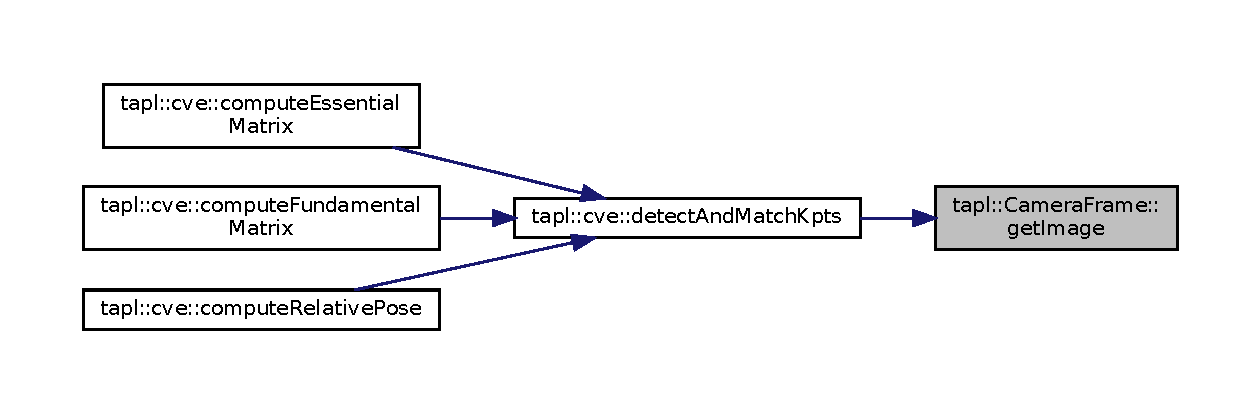
\includegraphics[width=350pt]{structtapl_1_1CameraFrame_a173bf0e309ba2a499425bb4d881c3a8f_icgraph}
\end{center}
\end{figure}
\mbox{\Hypertarget{structtapl_1_1CameraFrame_aafb04677ac368c41616786d74cada301}\label{structtapl_1_1CameraFrame_aafb04677ac368c41616786d74cada301}} 
\index{tapl::CameraFrame@{tapl::CameraFrame}!getKeypoints@{getKeypoints}}
\index{getKeypoints@{getKeypoints}!tapl::CameraFrame@{tapl::CameraFrame}}
\doxysubsubsection{\texorpdfstring{getKeypoints()}{getKeypoints()}}
{\footnotesize\ttfamily \mbox{\hyperlink{namespacetapl_a196ce1d5bf399fc26f03797e6a8d03ff}{Result\+Code}} tapl\+::\+Camera\+Frame\+::get\+Keypoints (\begin{DoxyParamCaption}\item[{std\+::vector$<$ cv\+::\+Key\+Point $>$ \&}]{keypoints }\end{DoxyParamCaption})\hspace{0.3cm}{\ttfamily [inline]}}



Definition at line 102 of file tapl\+Types.\+hpp.

Here is the caller graph for this function\+:\nopagebreak
\begin{figure}[H]
\begin{center}
\leavevmode
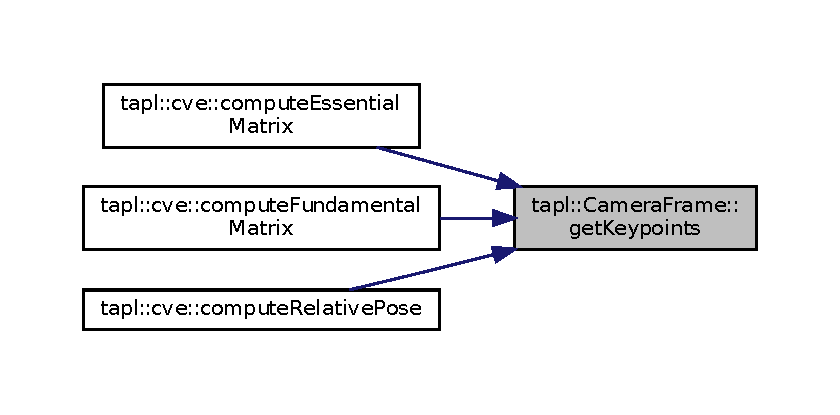
\includegraphics[width=350pt]{structtapl_1_1CameraFrame_aafb04677ac368c41616786d74cada301_icgraph}
\end{center}
\end{figure}
\mbox{\Hypertarget{structtapl_1_1CameraFrame_a8fb1c882c8586540cad9ed46e8e2c575}\label{structtapl_1_1CameraFrame_a8fb1c882c8586540cad9ed46e8e2c575}} 
\index{tapl::CameraFrame@{tapl::CameraFrame}!pushDescriptors@{pushDescriptors}}
\index{pushDescriptors@{pushDescriptors}!tapl::CameraFrame@{tapl::CameraFrame}}
\doxysubsubsection{\texorpdfstring{pushDescriptors()}{pushDescriptors()}}
{\footnotesize\ttfamily void tapl\+::\+Camera\+Frame\+::push\+Descriptors (\begin{DoxyParamCaption}\item[{cv\+::\+Mat \&}]{descriptors }\end{DoxyParamCaption})\hspace{0.3cm}{\ttfamily [inline]}}



Definition at line 87 of file tapl\+Types.\+hpp.

Here is the caller graph for this function\+:\nopagebreak
\begin{figure}[H]
\begin{center}
\leavevmode
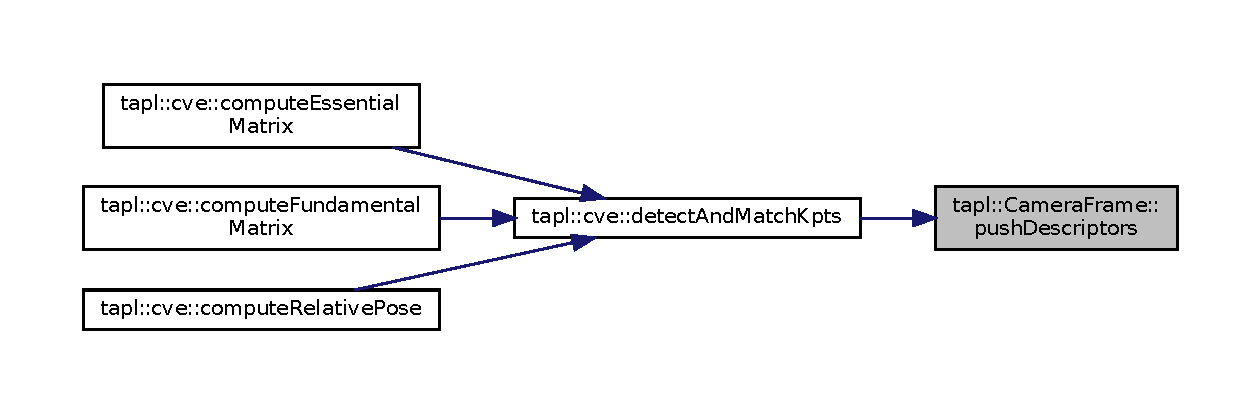
\includegraphics[width=350pt]{structtapl_1_1CameraFrame_a8fb1c882c8586540cad9ed46e8e2c575_icgraph}
\end{center}
\end{figure}
\mbox{\Hypertarget{structtapl_1_1CameraFrame_a3cd55417e231f33de32d6fe0491328f5}\label{structtapl_1_1CameraFrame_a3cd55417e231f33de32d6fe0491328f5}} 
\index{tapl::CameraFrame@{tapl::CameraFrame}!pushImage@{pushImage}}
\index{pushImage@{pushImage}!tapl::CameraFrame@{tapl::CameraFrame}}
\doxysubsubsection{\texorpdfstring{pushImage()}{pushImage()}}
{\footnotesize\ttfamily void tapl\+::\+Camera\+Frame\+::push\+Image (\begin{DoxyParamCaption}\item[{cv\+::\+Mat \&}]{img }\end{DoxyParamCaption})\hspace{0.3cm}{\ttfamily [inline]}}



Definition at line 83 of file tapl\+Types.\+hpp.

\mbox{\Hypertarget{structtapl_1_1CameraFrame_a615e5c9e86234c3a1ab0bff9385b2820}\label{structtapl_1_1CameraFrame_a615e5c9e86234c3a1ab0bff9385b2820}} 
\index{tapl::CameraFrame@{tapl::CameraFrame}!pushKeypoints@{pushKeypoints}}
\index{pushKeypoints@{pushKeypoints}!tapl::CameraFrame@{tapl::CameraFrame}}
\doxysubsubsection{\texorpdfstring{pushKeypoints()}{pushKeypoints()}}
{\footnotesize\ttfamily void tapl\+::\+Camera\+Frame\+::push\+Keypoints (\begin{DoxyParamCaption}\item[{std\+::vector$<$ cv\+::\+Key\+Point $>$ \&}]{keypoints }\end{DoxyParamCaption})\hspace{0.3cm}{\ttfamily [inline]}}



Definition at line 85 of file tapl\+Types.\+hpp.

Here is the caller graph for this function\+:\nopagebreak
\begin{figure}[H]
\begin{center}
\leavevmode
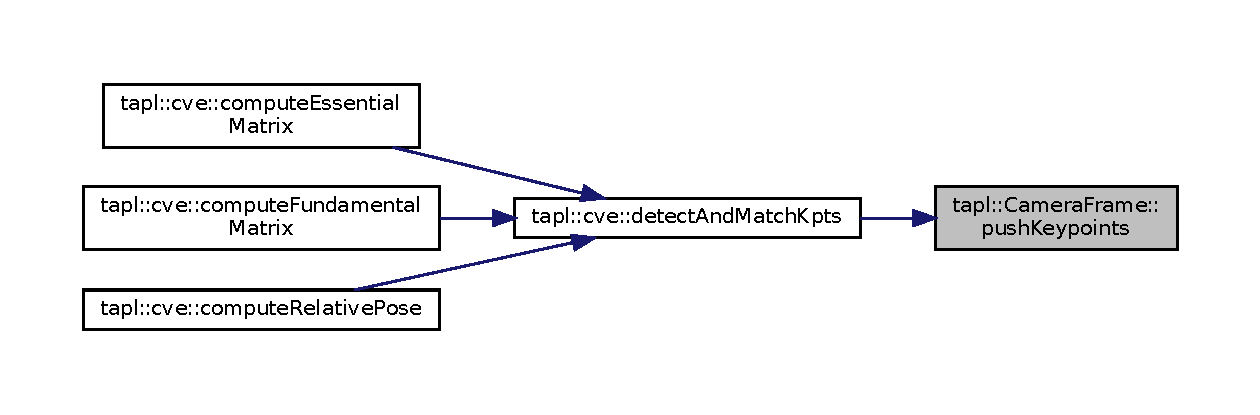
\includegraphics[width=350pt]{structtapl_1_1CameraFrame_a615e5c9e86234c3a1ab0bff9385b2820_icgraph}
\end{center}
\end{figure}


The documentation for this struct was generated from the following file\+:\begin{DoxyCompactItemize}
\item 
tapl/common/\mbox{\hyperlink{taplTypes_8hpp}{tapl\+Types.\+hpp}}\end{DoxyCompactItemize}

\hypertarget{structtapl_1_1DataFrame}{}\doxysection{tapl\+::Data\+Frame Struct Reference}
\label{structtapl_1_1DataFrame}\index{tapl::DataFrame@{tapl::DataFrame}}


represents the available sensor information at the same time instance  




{\ttfamily \#include $<$tapl\+Types.\+hpp$>$}



Collaboration diagram for tapl\+::Data\+Frame\+:
\nopagebreak
\begin{figure}[H]
\begin{center}
\leavevmode
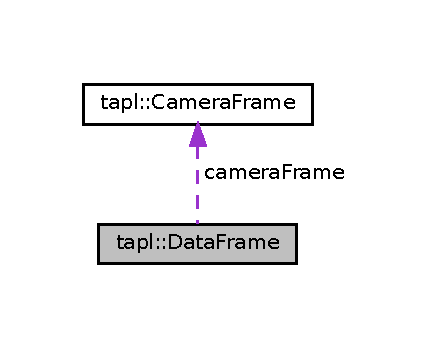
\includegraphics[width=230pt]{structtapl_1_1DataFrame__coll__graph}
\end{center}
\end{figure}
\doxysubsection*{Public Member Functions}
\begin{DoxyCompactItemize}
\item 
\mbox{\hyperlink{structtapl_1_1DataFrame_a046dcfff07492b3753902bc3bd924e1d}{Data\+Frame}} ()
\item 
void \mbox{\hyperlink{structtapl_1_1DataFrame_ab923cef38b00d4d67b5a480eb5e323e5}{push\+Kpts\+Matches}} (const std\+::vector$<$ cv\+::\+D\+Match $>$ \&kpt\+Matches)
\item 
void \mbox{\hyperlink{structtapl_1_1DataFrame_aea06402631517802fc36cd62f7b4ef52}{push\+Fundamental\+Matrix}} (const cv\+::\+Mat \&F)
\item 
void \mbox{\hyperlink{structtapl_1_1DataFrame_a9bf64f105e1ddc2e22d9b5c452a348d0}{push\+Essential\+Matrix}} (const cv\+::\+Mat \&E)
\item 
void \mbox{\hyperlink{structtapl_1_1DataFrame_ac040b5d4f9e337904920168b7e1242db}{push\+Pose}} (const \mbox{\hyperlink{structtapl_1_1Pose6dof}{Pose6dof}} \&pose)
\item 
void \mbox{\hyperlink{structtapl_1_1DataFrame_a234df0c976947072ebca8342b1c6b236}{push\+Triangulated\+Pts}} (const cv\+::\+Mat \&pts)
\item 
\mbox{\hyperlink{namespacetapl_a196ce1d5bf399fc26f03797e6a8d03ff}{Result\+Code}} \mbox{\hyperlink{structtapl_1_1DataFrame_abc568884baeeed4ff0576eef6e725f1a}{get\+Kpts\+Matches}} (std\+::vector$<$ cv\+::\+D\+Match $>$ \&kpt\+Matches) const
\item 
\mbox{\hyperlink{namespacetapl_a196ce1d5bf399fc26f03797e6a8d03ff}{Result\+Code}} \mbox{\hyperlink{structtapl_1_1DataFrame_a1d4c42241dccf8430457bf134a465440}{get\+Fundamental\+Matrix}} (cv\+::\+Mat \&F) const
\item 
\mbox{\hyperlink{namespacetapl_a196ce1d5bf399fc26f03797e6a8d03ff}{Result\+Code}} \mbox{\hyperlink{structtapl_1_1DataFrame_a62068412eaaf6c57b69622ed4c8de390}{get\+Essential\+Matrix}} (cv\+::\+Mat \&E) const
\item 
\mbox{\hyperlink{namespacetapl_a196ce1d5bf399fc26f03797e6a8d03ff}{Result\+Code}} \mbox{\hyperlink{structtapl_1_1DataFrame_a373a863b9d5ffb638bebaca02a1d8486}{get\+Pose}} (\mbox{\hyperlink{structtapl_1_1Pose6dof}{Pose6dof}} \&pose) const
\item 
\mbox{\hyperlink{namespacetapl_a196ce1d5bf399fc26f03797e6a8d03ff}{Result\+Code}} \mbox{\hyperlink{structtapl_1_1DataFrame_acdef86602755be2d9d09ea6515a0a1d4}{get\+Triangulated\+Points}} (cv\+::\+Mat \&pts) const
\end{DoxyCompactItemize}
\doxysubsection*{Data Fields}
\begin{DoxyCompactItemize}
\item 
\mbox{\hyperlink{structtapl_1_1CameraFrame}{Camera\+Frame}} \mbox{\hyperlink{structtapl_1_1DataFrame_a6a9523806fd3280ddd54085669572288}{camera\+Frame}}
\item 
\mbox{\hyperlink{structtapl_1_1CameraFrame}{Camera\+Frame}} $\ast$ \mbox{\hyperlink{structtapl_1_1DataFrame_a0360d64d27a7251c58e2ab5d30b01b3d}{other\+Camera\+Frame}}
\end{DoxyCompactItemize}


\doxysubsection{Detailed Description}
represents the available sensor information at the same time instance 

Definition at line 143 of file tapl\+Types.\+hpp.



\doxysubsection{Constructor \& Destructor Documentation}
\mbox{\Hypertarget{structtapl_1_1DataFrame_a046dcfff07492b3753902bc3bd924e1d}\label{structtapl_1_1DataFrame_a046dcfff07492b3753902bc3bd924e1d}} 
\index{tapl::DataFrame@{tapl::DataFrame}!DataFrame@{DataFrame}}
\index{DataFrame@{DataFrame}!tapl::DataFrame@{tapl::DataFrame}}
\doxysubsubsection{\texorpdfstring{DataFrame()}{DataFrame()}}
{\footnotesize\ttfamily tapl\+::\+Data\+Frame\+::\+Data\+Frame (\begin{DoxyParamCaption}{ }\end{DoxyParamCaption})\hspace{0.3cm}{\ttfamily [inline]}}

$<$ cunstructor 

Definition at line 158 of file tapl\+Types.\+hpp.



\doxysubsection{Member Function Documentation}
\mbox{\Hypertarget{structtapl_1_1DataFrame_a62068412eaaf6c57b69622ed4c8de390}\label{structtapl_1_1DataFrame_a62068412eaaf6c57b69622ed4c8de390}} 
\index{tapl::DataFrame@{tapl::DataFrame}!getEssentialMatrix@{getEssentialMatrix}}
\index{getEssentialMatrix@{getEssentialMatrix}!tapl::DataFrame@{tapl::DataFrame}}
\doxysubsubsection{\texorpdfstring{getEssentialMatrix()}{getEssentialMatrix()}}
{\footnotesize\ttfamily \mbox{\hyperlink{namespacetapl_a196ce1d5bf399fc26f03797e6a8d03ff}{Result\+Code}} tapl\+::\+Data\+Frame\+::get\+Essential\+Matrix (\begin{DoxyParamCaption}\item[{cv\+::\+Mat \&}]{E }\end{DoxyParamCaption}) const\hspace{0.3cm}{\ttfamily [inline]}}



Definition at line 204 of file tapl\+Types.\+hpp.

\mbox{\Hypertarget{structtapl_1_1DataFrame_a1d4c42241dccf8430457bf134a465440}\label{structtapl_1_1DataFrame_a1d4c42241dccf8430457bf134a465440}} 
\index{tapl::DataFrame@{tapl::DataFrame}!getFundamentalMatrix@{getFundamentalMatrix}}
\index{getFundamentalMatrix@{getFundamentalMatrix}!tapl::DataFrame@{tapl::DataFrame}}
\doxysubsubsection{\texorpdfstring{getFundamentalMatrix()}{getFundamentalMatrix()}}
{\footnotesize\ttfamily \mbox{\hyperlink{namespacetapl_a196ce1d5bf399fc26f03797e6a8d03ff}{Result\+Code}} tapl\+::\+Data\+Frame\+::get\+Fundamental\+Matrix (\begin{DoxyParamCaption}\item[{cv\+::\+Mat \&}]{F }\end{DoxyParamCaption}) const\hspace{0.3cm}{\ttfamily [inline]}}



Definition at line 193 of file tapl\+Types.\+hpp.

\mbox{\Hypertarget{structtapl_1_1DataFrame_abc568884baeeed4ff0576eef6e725f1a}\label{structtapl_1_1DataFrame_abc568884baeeed4ff0576eef6e725f1a}} 
\index{tapl::DataFrame@{tapl::DataFrame}!getKptsMatches@{getKptsMatches}}
\index{getKptsMatches@{getKptsMatches}!tapl::DataFrame@{tapl::DataFrame}}
\doxysubsubsection{\texorpdfstring{getKptsMatches()}{getKptsMatches()}}
{\footnotesize\ttfamily \mbox{\hyperlink{namespacetapl_a196ce1d5bf399fc26f03797e6a8d03ff}{Result\+Code}} tapl\+::\+Data\+Frame\+::get\+Kpts\+Matches (\begin{DoxyParamCaption}\item[{std\+::vector$<$ cv\+::\+D\+Match $>$ \&}]{kpt\+Matches }\end{DoxyParamCaption}) const\hspace{0.3cm}{\ttfamily [inline]}}



Definition at line 182 of file tapl\+Types.\+hpp.

Here is the caller graph for this function\+:
\nopagebreak
\begin{figure}[H]
\begin{center}
\leavevmode
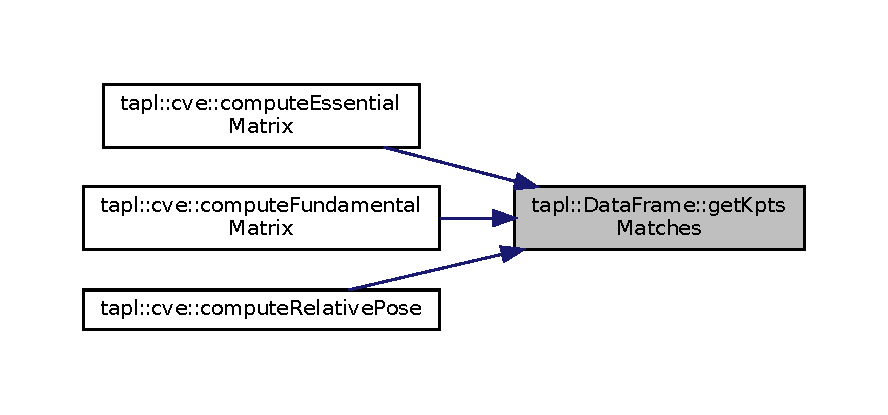
\includegraphics[width=350pt]{structtapl_1_1DataFrame_abc568884baeeed4ff0576eef6e725f1a_icgraph}
\end{center}
\end{figure}
\mbox{\Hypertarget{structtapl_1_1DataFrame_a373a863b9d5ffb638bebaca02a1d8486}\label{structtapl_1_1DataFrame_a373a863b9d5ffb638bebaca02a1d8486}} 
\index{tapl::DataFrame@{tapl::DataFrame}!getPose@{getPose}}
\index{getPose@{getPose}!tapl::DataFrame@{tapl::DataFrame}}
\doxysubsubsection{\texorpdfstring{getPose()}{getPose()}}
{\footnotesize\ttfamily \mbox{\hyperlink{namespacetapl_a196ce1d5bf399fc26f03797e6a8d03ff}{Result\+Code}} tapl\+::\+Data\+Frame\+::get\+Pose (\begin{DoxyParamCaption}\item[{\mbox{\hyperlink{structtapl_1_1Pose6dof}{Pose6dof}} \&}]{pose }\end{DoxyParamCaption}) const\hspace{0.3cm}{\ttfamily [inline]}}



Definition at line 215 of file tapl\+Types.\+hpp.

\mbox{\Hypertarget{structtapl_1_1DataFrame_acdef86602755be2d9d09ea6515a0a1d4}\label{structtapl_1_1DataFrame_acdef86602755be2d9d09ea6515a0a1d4}} 
\index{tapl::DataFrame@{tapl::DataFrame}!getTriangulatedPoints@{getTriangulatedPoints}}
\index{getTriangulatedPoints@{getTriangulatedPoints}!tapl::DataFrame@{tapl::DataFrame}}
\doxysubsubsection{\texorpdfstring{getTriangulatedPoints()}{getTriangulatedPoints()}}
{\footnotesize\ttfamily \mbox{\hyperlink{namespacetapl_a196ce1d5bf399fc26f03797e6a8d03ff}{Result\+Code}} tapl\+::\+Data\+Frame\+::get\+Triangulated\+Points (\begin{DoxyParamCaption}\item[{cv\+::\+Mat \&}]{pts }\end{DoxyParamCaption}) const\hspace{0.3cm}{\ttfamily [inline]}}



Definition at line 226 of file tapl\+Types.\+hpp.

\mbox{\Hypertarget{structtapl_1_1DataFrame_a9bf64f105e1ddc2e22d9b5c452a348d0}\label{structtapl_1_1DataFrame_a9bf64f105e1ddc2e22d9b5c452a348d0}} 
\index{tapl::DataFrame@{tapl::DataFrame}!pushEssentialMatrix@{pushEssentialMatrix}}
\index{pushEssentialMatrix@{pushEssentialMatrix}!tapl::DataFrame@{tapl::DataFrame}}
\doxysubsubsection{\texorpdfstring{pushEssentialMatrix()}{pushEssentialMatrix()}}
{\footnotesize\ttfamily void tapl\+::\+Data\+Frame\+::push\+Essential\+Matrix (\begin{DoxyParamCaption}\item[{const cv\+::\+Mat \&}]{E }\end{DoxyParamCaption})\hspace{0.3cm}{\ttfamily [inline]}}



Definition at line 174 of file tapl\+Types.\+hpp.

Here is the caller graph for this function\+:
\nopagebreak
\begin{figure}[H]
\begin{center}
\leavevmode
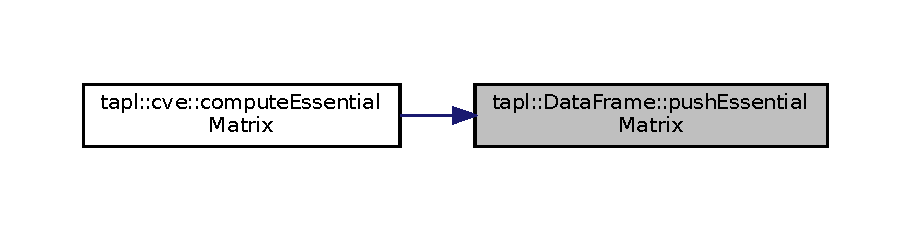
\includegraphics[width=350pt]{structtapl_1_1DataFrame_a9bf64f105e1ddc2e22d9b5c452a348d0_icgraph}
\end{center}
\end{figure}
\mbox{\Hypertarget{structtapl_1_1DataFrame_aea06402631517802fc36cd62f7b4ef52}\label{structtapl_1_1DataFrame_aea06402631517802fc36cd62f7b4ef52}} 
\index{tapl::DataFrame@{tapl::DataFrame}!pushFundamentalMatrix@{pushFundamentalMatrix}}
\index{pushFundamentalMatrix@{pushFundamentalMatrix}!tapl::DataFrame@{tapl::DataFrame}}
\doxysubsubsection{\texorpdfstring{pushFundamentalMatrix()}{pushFundamentalMatrix()}}
{\footnotesize\ttfamily void tapl\+::\+Data\+Frame\+::push\+Fundamental\+Matrix (\begin{DoxyParamCaption}\item[{const cv\+::\+Mat \&}]{F }\end{DoxyParamCaption})\hspace{0.3cm}{\ttfamily [inline]}}



Definition at line 172 of file tapl\+Types.\+hpp.

Here is the caller graph for this function\+:
\nopagebreak
\begin{figure}[H]
\begin{center}
\leavevmode
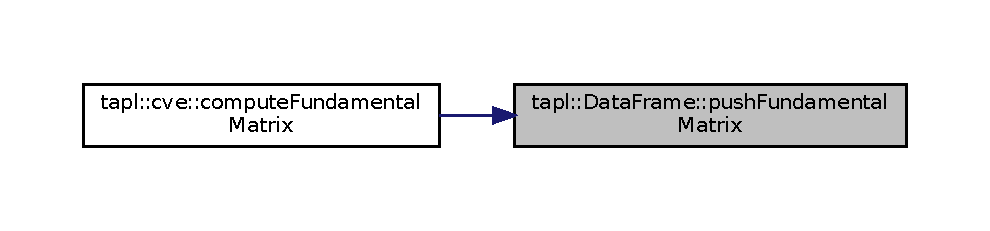
\includegraphics[width=350pt]{structtapl_1_1DataFrame_aea06402631517802fc36cd62f7b4ef52_icgraph}
\end{center}
\end{figure}
\mbox{\Hypertarget{structtapl_1_1DataFrame_ab923cef38b00d4d67b5a480eb5e323e5}\label{structtapl_1_1DataFrame_ab923cef38b00d4d67b5a480eb5e323e5}} 
\index{tapl::DataFrame@{tapl::DataFrame}!pushKptsMatches@{pushKptsMatches}}
\index{pushKptsMatches@{pushKptsMatches}!tapl::DataFrame@{tapl::DataFrame}}
\doxysubsubsection{\texorpdfstring{pushKptsMatches()}{pushKptsMatches()}}
{\footnotesize\ttfamily void tapl\+::\+Data\+Frame\+::push\+Kpts\+Matches (\begin{DoxyParamCaption}\item[{const std\+::vector$<$ cv\+::\+D\+Match $>$ \&}]{kpt\+Matches }\end{DoxyParamCaption})\hspace{0.3cm}{\ttfamily [inline]}}



Definition at line 170 of file tapl\+Types.\+hpp.

Here is the caller graph for this function\+:
\nopagebreak
\begin{figure}[H]
\begin{center}
\leavevmode
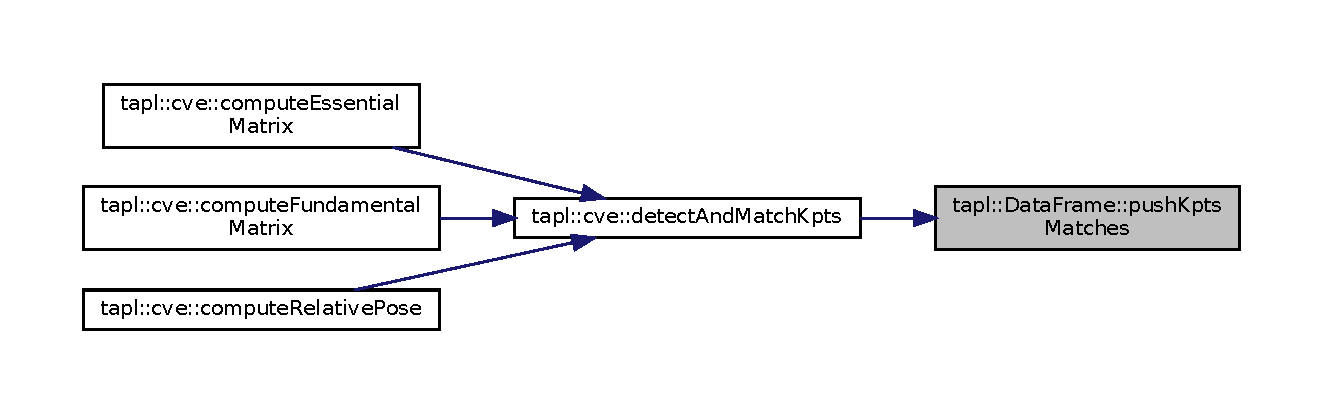
\includegraphics[width=350pt]{structtapl_1_1DataFrame_ab923cef38b00d4d67b5a480eb5e323e5_icgraph}
\end{center}
\end{figure}
\mbox{\Hypertarget{structtapl_1_1DataFrame_ac040b5d4f9e337904920168b7e1242db}\label{structtapl_1_1DataFrame_ac040b5d4f9e337904920168b7e1242db}} 
\index{tapl::DataFrame@{tapl::DataFrame}!pushPose@{pushPose}}
\index{pushPose@{pushPose}!tapl::DataFrame@{tapl::DataFrame}}
\doxysubsubsection{\texorpdfstring{pushPose()}{pushPose()}}
{\footnotesize\ttfamily void tapl\+::\+Data\+Frame\+::push\+Pose (\begin{DoxyParamCaption}\item[{const \mbox{\hyperlink{structtapl_1_1Pose6dof}{Pose6dof}} \&}]{pose }\end{DoxyParamCaption})\hspace{0.3cm}{\ttfamily [inline]}}



Definition at line 176 of file tapl\+Types.\+hpp.

Here is the caller graph for this function\+:
\nopagebreak
\begin{figure}[H]
\begin{center}
\leavevmode
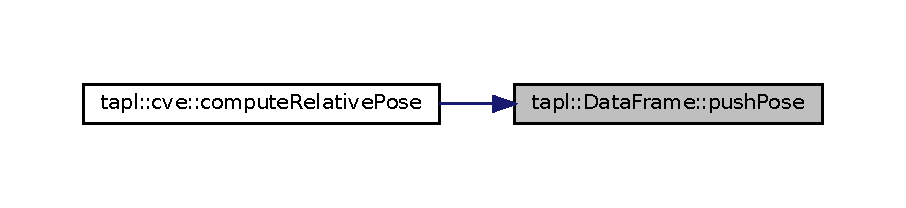
\includegraphics[width=350pt]{structtapl_1_1DataFrame_ac040b5d4f9e337904920168b7e1242db_icgraph}
\end{center}
\end{figure}
\mbox{\Hypertarget{structtapl_1_1DataFrame_a234df0c976947072ebca8342b1c6b236}\label{structtapl_1_1DataFrame_a234df0c976947072ebca8342b1c6b236}} 
\index{tapl::DataFrame@{tapl::DataFrame}!pushTriangulatedPts@{pushTriangulatedPts}}
\index{pushTriangulatedPts@{pushTriangulatedPts}!tapl::DataFrame@{tapl::DataFrame}}
\doxysubsubsection{\texorpdfstring{pushTriangulatedPts()}{pushTriangulatedPts()}}
{\footnotesize\ttfamily void tapl\+::\+Data\+Frame\+::push\+Triangulated\+Pts (\begin{DoxyParamCaption}\item[{const cv\+::\+Mat \&}]{pts }\end{DoxyParamCaption})\hspace{0.3cm}{\ttfamily [inline]}}



Definition at line 178 of file tapl\+Types.\+hpp.

Here is the caller graph for this function\+:
\nopagebreak
\begin{figure}[H]
\begin{center}
\leavevmode
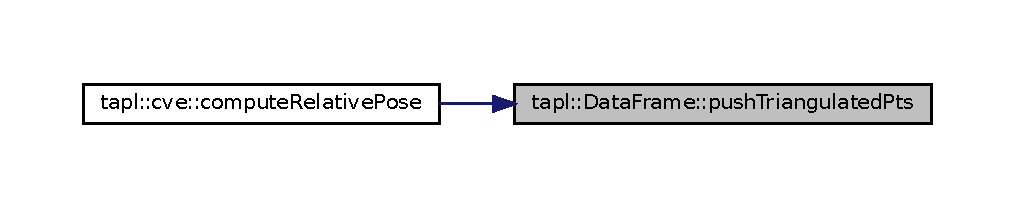
\includegraphics[width=350pt]{structtapl_1_1DataFrame_a234df0c976947072ebca8342b1c6b236_icgraph}
\end{center}
\end{figure}


\doxysubsection{Field Documentation}
\mbox{\Hypertarget{structtapl_1_1DataFrame_a6a9523806fd3280ddd54085669572288}\label{structtapl_1_1DataFrame_a6a9523806fd3280ddd54085669572288}} 
\index{tapl::DataFrame@{tapl::DataFrame}!cameraFrame@{cameraFrame}}
\index{cameraFrame@{cameraFrame}!tapl::DataFrame@{tapl::DataFrame}}
\doxysubsubsection{\texorpdfstring{cameraFrame}{cameraFrame}}
{\footnotesize\ttfamily \mbox{\hyperlink{structtapl_1_1CameraFrame}{Camera\+Frame}} tapl\+::\+Data\+Frame\+::camera\+Frame}

Image frame 

Definition at line 165 of file tapl\+Types.\+hpp.

\mbox{\Hypertarget{structtapl_1_1DataFrame_a0360d64d27a7251c58e2ab5d30b01b3d}\label{structtapl_1_1DataFrame_a0360d64d27a7251c58e2ab5d30b01b3d}} 
\index{tapl::DataFrame@{tapl::DataFrame}!otherCameraFrame@{otherCameraFrame}}
\index{otherCameraFrame@{otherCameraFrame}!tapl::DataFrame@{tapl::DataFrame}}
\doxysubsubsection{\texorpdfstring{otherCameraFrame}{otherCameraFrame}}
{\footnotesize\ttfamily \mbox{\hyperlink{structtapl_1_1CameraFrame}{Camera\+Frame}}$\ast$ tapl\+::\+Data\+Frame\+::other\+Camera\+Frame}

Other image frame used for computing F, E, etc. 

Definition at line 166 of file tapl\+Types.\+hpp.



The documentation for this struct was generated from the following file\+:\begin{DoxyCompactItemize}
\item 
tapl/common/\mbox{\hyperlink{taplTypes_8hpp}{tapl\+Types.\+hpp}}\end{DoxyCompactItemize}

\hypertarget{classtapl_1_1pte_1_1EuclideanCluster}{}\section{tapl\+:\+:pte\+:\+:Euclidean\+Cluster Class Reference}
\label{classtapl_1_1pte_1_1EuclideanCluster}\index{tapl\+::pte\+::\+Euclidean\+Cluster@{tapl\+::pte\+::\+Euclidean\+Cluster}}


{\ttfamily \#include $<$pt\+Engine.\+hpp$>$}

\subsection*{Public Member Functions}
\begin{DoxyCompactItemize}
\item 
\hyperlink{classtapl_1_1pte_1_1EuclideanCluster_ae0cc79c58e5c58512b953c9252acfcb0}{Euclidean\+Cluster} (const std\+::vector$<$ std\+::vector$<$ float $>$$>$ \&points, \hyperlink{structtapl_1_1pte_1_1KdTree}{Kd\+Tree} $\ast$tree)
\item 
std\+::vector$<$ std\+::vector$<$ int $>$ $>$ \hyperlink{classtapl_1_1pte_1_1EuclideanCluster_a7006b8b1a10af362b0001e4f36d3b4fb}{clustering} (float dist\+Tolerance)
\end{DoxyCompactItemize}


\subsection{Detailed Description}


Definition at line 112 of file pt\+Engine.\+hpp.



\subsection{Constructor \& Destructor Documentation}
\index{tapl\+::pte\+::\+Euclidean\+Cluster@{tapl\+::pte\+::\+Euclidean\+Cluster}!Euclidean\+Cluster@{Euclidean\+Cluster}}
\index{Euclidean\+Cluster@{Euclidean\+Cluster}!tapl\+::pte\+::\+Euclidean\+Cluster@{tapl\+::pte\+::\+Euclidean\+Cluster}}
\subsubsection[{\texorpdfstring{Euclidean\+Cluster(const std\+::vector$<$ std\+::vector$<$ float $>$$>$ \&points, Kd\+Tree $\ast$tree)}{EuclideanCluster(const std::vector< std::vector< float >> &points, KdTree *tree)}}]{\setlength{\rightskip}{0pt plus 5cm}tapl\+::pte\+::\+Euclidean\+Cluster\+::\+Euclidean\+Cluster (
\begin{DoxyParamCaption}
\item[{const std\+::vector$<$ std\+::vector$<$ float $>$$>$ \&}]{points, }
\item[{{\bf Kd\+Tree} $\ast$}]{tree}
\end{DoxyParamCaption}
)\hspace{0.3cm}{\ttfamily [inline]}}\hypertarget{classtapl_1_1pte_1_1EuclideanCluster_ae0cc79c58e5c58512b953c9252acfcb0}{}\label{classtapl_1_1pte_1_1EuclideanCluster_ae0cc79c58e5c58512b953c9252acfcb0}


Definition at line 115 of file pt\+Engine.\+hpp.



\subsection{Member Function Documentation}
\index{tapl\+::pte\+::\+Euclidean\+Cluster@{tapl\+::pte\+::\+Euclidean\+Cluster}!clustering@{clustering}}
\index{clustering@{clustering}!tapl\+::pte\+::\+Euclidean\+Cluster@{tapl\+::pte\+::\+Euclidean\+Cluster}}
\subsubsection[{\texorpdfstring{clustering(float dist\+Tolerance)}{clustering(float distTolerance)}}]{\setlength{\rightskip}{0pt plus 5cm}std\+::vector$<$ std\+::vector$<$ int $>$ $>$ tapl\+::pte\+::\+Euclidean\+Cluster\+::clustering (
\begin{DoxyParamCaption}
\item[{float}]{dist\+Tolerance}
\end{DoxyParamCaption}
)}\hypertarget{classtapl_1_1pte_1_1EuclideanCluster_a7006b8b1a10af362b0001e4f36d3b4fb}{}\label{classtapl_1_1pte_1_1EuclideanCluster_a7006b8b1a10af362b0001e4f36d3b4fb}


Definition at line 417 of file pt\+Engine.\+cpp.



Here is the caller graph for this function\+:\nopagebreak
\begin{figure}[H]
\begin{center}
\leavevmode
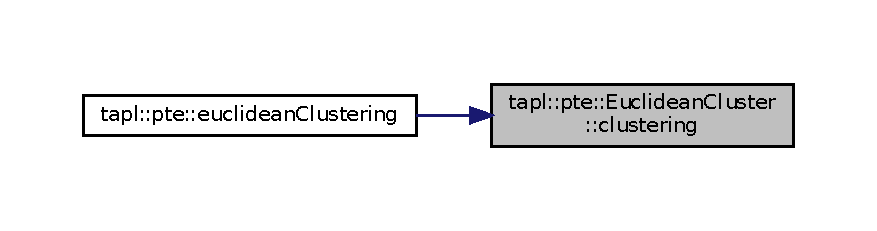
\includegraphics[width=350pt]{classtapl_1_1pte_1_1EuclideanCluster_a7006b8b1a10af362b0001e4f36d3b4fb_icgraph}
\end{center}
\end{figure}




The documentation for this class was generated from the following files\+:\begin{DoxyCompactItemize}
\item 
tapl/\hyperlink{ptEngine_8hpp}{pt\+Engine.\+hpp}\item 
tapl/\hyperlink{ptEngine_8cpp}{pt\+Engine.\+cpp}\end{DoxyCompactItemize}

\hypertarget{structtapl_1_1pte_1_1KdTree}{}\doxysection{tapl\+::pte\+::Kd\+Tree Struct Reference}
\label{structtapl_1_1pte_1_1KdTree}\index{tapl::pte::KdTree@{tapl::pte::KdTree}}


{\ttfamily \#include $<$pt\+Engine.\+hpp$>$}



Collaboration diagram for tapl\+::pte\+::Kd\+Tree\+:
\nopagebreak
\begin{figure}[H]
\begin{center}
\leavevmode
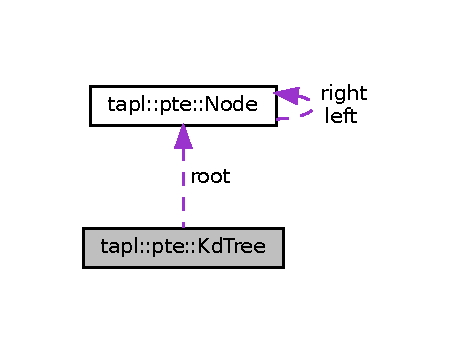
\includegraphics[width=217pt]{structtapl_1_1pte_1_1KdTree__coll__graph}
\end{center}
\end{figure}
\doxysubsection*{Public Member Functions}
\begin{DoxyCompactItemize}
\item 
\mbox{\hyperlink{structtapl_1_1pte_1_1KdTree_a2b25b4997076cce12e0c3b38ed8217fe}{Kd\+Tree}} ()
\item 
void \mbox{\hyperlink{structtapl_1_1pte_1_1KdTree_acaf4969659031fa301d1b7e46d6b3b77}{insert}} (std\+::vector$<$ float $>$ point, int id)
\item 
std\+::vector$<$ int $>$ \mbox{\hyperlink{structtapl_1_1pte_1_1KdTree_a99b69a039013a6bbc2be7041190168b1}{search}} (std\+::vector$<$ float $>$ target, float dist\+Tolerance)
\item 
float \mbox{\hyperlink{structtapl_1_1pte_1_1KdTree_a58fd56f5fcbc48ec95e975cc02471d1b}{dist}} (std\+::vector$<$ float $>$ point\+\_\+a, std\+::vector$<$ float $>$ point\+\_\+b)
\item 
void \mbox{\hyperlink{structtapl_1_1pte_1_1KdTree_a388598d62bc5f21a5f5b802a8feecc74}{insert\+Helper}} (\mbox{\hyperlink{structtapl_1_1pte_1_1Node}{Node}} $\ast$$\ast$node, unsigned depth, std\+::vector$<$ float $>$ point, int id)
\item 
void \mbox{\hyperlink{structtapl_1_1pte_1_1KdTree_a8add21f54b1f0ee01746582073e9fac5}{search\+Helper}} (\mbox{\hyperlink{structtapl_1_1pte_1_1Node}{Node}} $\ast$node, std\+::vector$<$ float $>$ target, float dist\+Tolerance, int depth, std\+::vector$<$ int $>$ \&ids)
\end{DoxyCompactItemize}
\doxysubsection*{Data Fields}
\begin{DoxyCompactItemize}
\item 
\mbox{\hyperlink{structtapl_1_1pte_1_1Node}{Node}} $\ast$ \mbox{\hyperlink{structtapl_1_1pte_1_1KdTree_a5dd05133b3a9429ae973eda1806c05e7}{root}}
\end{DoxyCompactItemize}


\doxysubsection{Detailed Description}


Definition at line 89 of file pt\+Engine.\+hpp.



\doxysubsection{Constructor \& Destructor Documentation}
\mbox{\Hypertarget{structtapl_1_1pte_1_1KdTree_a2b25b4997076cce12e0c3b38ed8217fe}\label{structtapl_1_1pte_1_1KdTree_a2b25b4997076cce12e0c3b38ed8217fe}} 
\index{tapl::pte::KdTree@{tapl::pte::KdTree}!KdTree@{KdTree}}
\index{KdTree@{KdTree}!tapl::pte::KdTree@{tapl::pte::KdTree}}
\doxysubsubsection{\texorpdfstring{KdTree()}{KdTree()}}
{\footnotesize\ttfamily tapl\+::pte\+::\+Kd\+Tree\+::\+Kd\+Tree (\begin{DoxyParamCaption}{ }\end{DoxyParamCaption})\hspace{0.3cm}{\ttfamily [inline]}}



Definition at line 94 of file pt\+Engine.\+hpp.



\doxysubsection{Member Function Documentation}
\mbox{\Hypertarget{structtapl_1_1pte_1_1KdTree_a58fd56f5fcbc48ec95e975cc02471d1b}\label{structtapl_1_1pte_1_1KdTree_a58fd56f5fcbc48ec95e975cc02471d1b}} 
\index{tapl::pte::KdTree@{tapl::pte::KdTree}!dist@{dist}}
\index{dist@{dist}!tapl::pte::KdTree@{tapl::pte::KdTree}}
\doxysubsubsection{\texorpdfstring{dist()}{dist()}}
{\footnotesize\ttfamily float tapl\+::pte\+::\+Kd\+Tree\+::dist (\begin{DoxyParamCaption}\item[{std\+::vector$<$ float $>$}]{point\+\_\+a,  }\item[{std\+::vector$<$ float $>$}]{point\+\_\+b }\end{DoxyParamCaption})}



Definition at line 367 of file pt\+Engine.\+cpp.

Here is the caller graph for this function\+:
\nopagebreak
\begin{figure}[H]
\begin{center}
\leavevmode
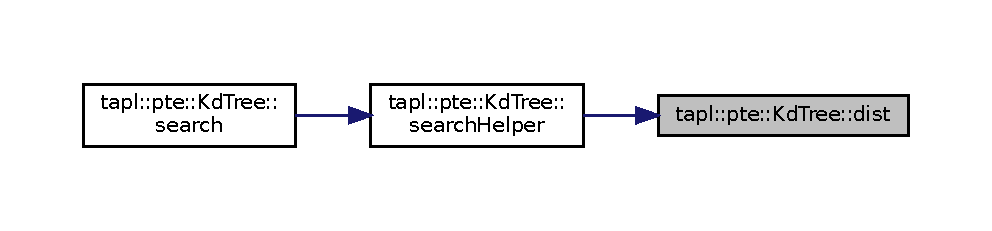
\includegraphics[width=350pt]{structtapl_1_1pte_1_1KdTree_a58fd56f5fcbc48ec95e975cc02471d1b_icgraph}
\end{center}
\end{figure}
\mbox{\Hypertarget{structtapl_1_1pte_1_1KdTree_acaf4969659031fa301d1b7e46d6b3b77}\label{structtapl_1_1pte_1_1KdTree_acaf4969659031fa301d1b7e46d6b3b77}} 
\index{tapl::pte::KdTree@{tapl::pte::KdTree}!insert@{insert}}
\index{insert@{insert}!tapl::pte::KdTree@{tapl::pte::KdTree}}
\doxysubsubsection{\texorpdfstring{insert()}{insert()}}
{\footnotesize\ttfamily void tapl\+::pte\+::\+Kd\+Tree\+::insert (\begin{DoxyParamCaption}\item[{std\+::vector$<$ float $>$}]{point,  }\item[{int}]{id }\end{DoxyParamCaption})}



Definition at line 359 of file pt\+Engine.\+cpp.

Here is the call graph for this function\+:
\nopagebreak
\begin{figure}[H]
\begin{center}
\leavevmode
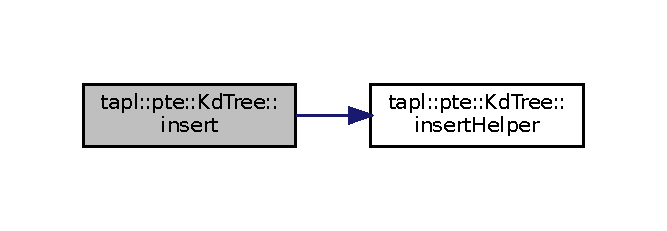
\includegraphics[width=320pt]{structtapl_1_1pte_1_1KdTree_acaf4969659031fa301d1b7e46d6b3b77_cgraph}
\end{center}
\end{figure}
Here is the caller graph for this function\+:
\nopagebreak
\begin{figure}[H]
\begin{center}
\leavevmode
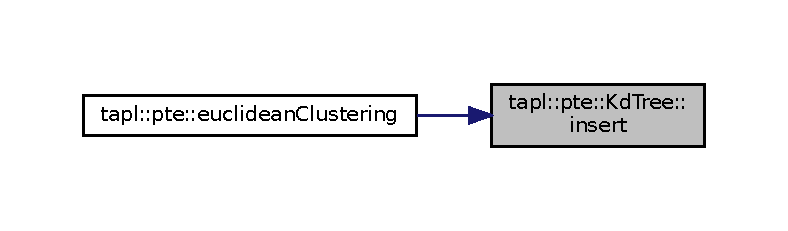
\includegraphics[width=350pt]{structtapl_1_1pte_1_1KdTree_acaf4969659031fa301d1b7e46d6b3b77_icgraph}
\end{center}
\end{figure}
\mbox{\Hypertarget{structtapl_1_1pte_1_1KdTree_a388598d62bc5f21a5f5b802a8feecc74}\label{structtapl_1_1pte_1_1KdTree_a388598d62bc5f21a5f5b802a8feecc74}} 
\index{tapl::pte::KdTree@{tapl::pte::KdTree}!insertHelper@{insertHelper}}
\index{insertHelper@{insertHelper}!tapl::pte::KdTree@{tapl::pte::KdTree}}
\doxysubsubsection{\texorpdfstring{insertHelper()}{insertHelper()}}
{\footnotesize\ttfamily void tapl\+::pte\+::\+Kd\+Tree\+::insert\+Helper (\begin{DoxyParamCaption}\item[{\mbox{\hyperlink{structtapl_1_1pte_1_1Node}{Node}} $\ast$$\ast$}]{node,  }\item[{unsigned}]{depth,  }\item[{std\+::vector$<$ float $>$}]{point,  }\item[{int}]{id }\end{DoxyParamCaption})}



Definition at line 338 of file pt\+Engine.\+cpp.

Here is the caller graph for this function\+:
\nopagebreak
\begin{figure}[H]
\begin{center}
\leavevmode
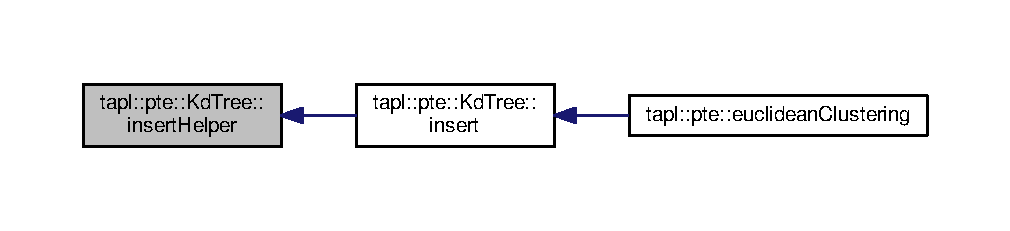
\includegraphics[width=350pt]{structtapl_1_1pte_1_1KdTree_a388598d62bc5f21a5f5b802a8feecc74_icgraph}
\end{center}
\end{figure}
\mbox{\Hypertarget{structtapl_1_1pte_1_1KdTree_a99b69a039013a6bbc2be7041190168b1}\label{structtapl_1_1pte_1_1KdTree_a99b69a039013a6bbc2be7041190168b1}} 
\index{tapl::pte::KdTree@{tapl::pte::KdTree}!search@{search}}
\index{search@{search}!tapl::pte::KdTree@{tapl::pte::KdTree}}
\doxysubsubsection{\texorpdfstring{search()}{search()}}
{\footnotesize\ttfamily std\+::vector$<$ int $>$ tapl\+::pte\+::\+Kd\+Tree\+::search (\begin{DoxyParamCaption}\item[{std\+::vector$<$ float $>$}]{target,  }\item[{float}]{dist\+Tolerance }\end{DoxyParamCaption})}



Definition at line 394 of file pt\+Engine.\+cpp.

Here is the call graph for this function\+:
\nopagebreak
\begin{figure}[H]
\begin{center}
\leavevmode
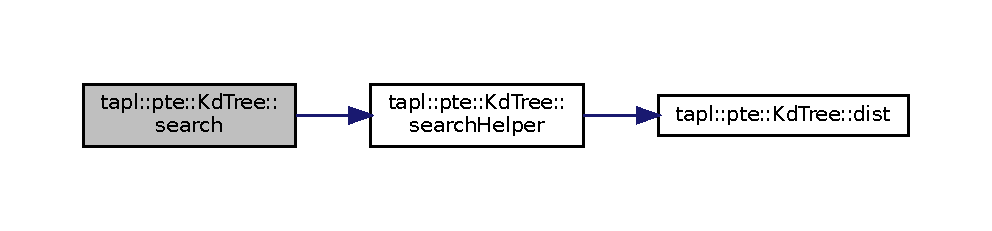
\includegraphics[width=350pt]{structtapl_1_1pte_1_1KdTree_a99b69a039013a6bbc2be7041190168b1_cgraph}
\end{center}
\end{figure}
\mbox{\Hypertarget{structtapl_1_1pte_1_1KdTree_a8add21f54b1f0ee01746582073e9fac5}\label{structtapl_1_1pte_1_1KdTree_a8add21f54b1f0ee01746582073e9fac5}} 
\index{tapl::pte::KdTree@{tapl::pte::KdTree}!searchHelper@{searchHelper}}
\index{searchHelper@{searchHelper}!tapl::pte::KdTree@{tapl::pte::KdTree}}
\doxysubsubsection{\texorpdfstring{searchHelper()}{searchHelper()}}
{\footnotesize\ttfamily void tapl\+::pte\+::\+Kd\+Tree\+::search\+Helper (\begin{DoxyParamCaption}\item[{\mbox{\hyperlink{structtapl_1_1pte_1_1Node}{Node}} $\ast$}]{node,  }\item[{std\+::vector$<$ float $>$}]{target,  }\item[{float}]{dist\+Tolerance,  }\item[{int}]{depth,  }\item[{std\+::vector$<$ int $>$ \&}]{ids }\end{DoxyParamCaption})}



Definition at line 378 of file pt\+Engine.\+cpp.

Here is the call graph for this function\+:
\nopagebreak
\begin{figure}[H]
\begin{center}
\leavevmode
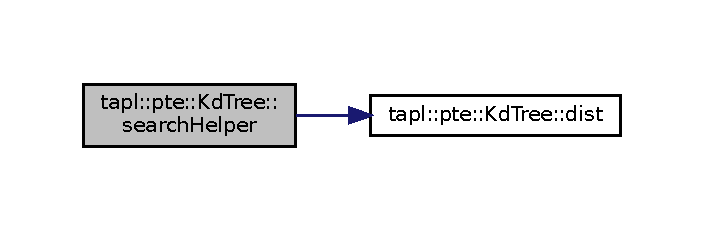
\includegraphics[width=338pt]{structtapl_1_1pte_1_1KdTree_a8add21f54b1f0ee01746582073e9fac5_cgraph}
\end{center}
\end{figure}
Here is the caller graph for this function\+:
\nopagebreak
\begin{figure}[H]
\begin{center}
\leavevmode

\includegraphics[width=320pt]{structtapl_1_1pte_1_1KdTree_a8add21f54b1f0ee01746582073e9fac5_icgraph}
\end{center}
\end{figure}


\doxysubsection{Field Documentation}
\mbox{\Hypertarget{structtapl_1_1pte_1_1KdTree_a5dd05133b3a9429ae973eda1806c05e7}\label{structtapl_1_1pte_1_1KdTree_a5dd05133b3a9429ae973eda1806c05e7}} 
\index{tapl::pte::KdTree@{tapl::pte::KdTree}!root@{root}}
\index{root@{root}!tapl::pte::KdTree@{tapl::pte::KdTree}}
\doxysubsubsection{\texorpdfstring{root}{root}}
{\footnotesize\ttfamily \mbox{\hyperlink{structtapl_1_1pte_1_1Node}{Node}}$\ast$ tapl\+::pte\+::\+Kd\+Tree\+::root}



Definition at line 91 of file pt\+Engine.\+hpp.



The documentation for this struct was generated from the following files\+:\begin{DoxyCompactItemize}
\item 
tapl/pte/\mbox{\hyperlink{ptEngine_8hpp}{pt\+Engine.\+hpp}}\item 
tapl/pte/\mbox{\hyperlink{ptEngine_8cpp}{pt\+Engine.\+cpp}}\end{DoxyCompactItemize}

\hypertarget{classtapl_1_1pte_1_1Line}{}\section{tapl\+:\+:pte\+:\+:Line$<$ PointT $>$ Class Template Reference}
\label{classtapl_1_1pte_1_1Line}\index{tapl\+::pte\+::\+Line$<$ Point\+T $>$@{tapl\+::pte\+::\+Line$<$ Point\+T $>$}}


{\ttfamily \#include $<$pt\+Engine.\+hpp$>$}

\subsection*{Public Member Functions}
\begin{DoxyCompactItemize}
\item 
\hyperlink{classtapl_1_1pte_1_1Line_a3484fb0de3bc1bcf2bb22b4943330979}{Line} ()
\item 
\hyperlink{classtapl_1_1pte_1_1Line_a3ef1f4fbb2ae11c564176fffc4befe74}{$\sim$\+Line} ()
\item 
std\+::vector$<$ float $>$ \hyperlink{classtapl_1_1pte_1_1Line_aa1de142cfa7dd5b26093a99df05d9f8c}{fit\+S\+VD} (std\+::vector$<$ float $>$ \&x, std\+::vector$<$ float $>$ \&y)
\item 
std\+::vector$<$ float $>$ \hyperlink{classtapl_1_1pte_1_1Line_a705b09b731117dae2d47d91a423ff828}{fit\+LS} (std\+::vector$<$ float $>$ \&x, std\+::vector$<$ float $>$ \&y)
\item 
float \hyperlink{classtapl_1_1pte_1_1Line_a97f6d7505cead12ac6f82d84ca0bf92a}{dist\+To\+Point} (std\+::vector$<$ float $>$ line\+\_\+coeffs, PointT point)
\item 
std\+::unordered\+\_\+set$<$ int $>$ \hyperlink{classtapl_1_1pte_1_1Line_a50a79f0b345fd3b9fb830a035ccf8e1d}{Ransac} (typename pcl\+::\+Point\+Cloud$<$ PointT $>$\+::Ptr cloud, int max\+Iterations, float distance\+Tol)
\end{DoxyCompactItemize}


\subsection{Detailed Description}
\subsubsection*{template$<$typename PointT$>$\\*
class tapl\+::pte\+::\+Line$<$ Point\+T $>$}



Definition at line 33 of file pt\+Engine.\+hpp.



\subsection{Constructor \& Destructor Documentation}
\index{tapl\+::pte\+::\+Line@{tapl\+::pte\+::\+Line}!Line@{Line}}
\index{Line@{Line}!tapl\+::pte\+::\+Line@{tapl\+::pte\+::\+Line}}
\subsubsection[{\texorpdfstring{Line()}{Line()}}]{\setlength{\rightskip}{0pt plus 5cm}template$<$typename PointT $>$ {\bf tapl\+::pte\+::\+Line}$<$ PointT $>$\+::{\bf Line} (
\begin{DoxyParamCaption}
{}
\end{DoxyParamCaption}
)}\hypertarget{classtapl_1_1pte_1_1Line_a3484fb0de3bc1bcf2bb22b4943330979}{}\label{classtapl_1_1pte_1_1Line_a3484fb0de3bc1bcf2bb22b4943330979}


Definition at line 8 of file pt\+Engine.\+cpp.

\index{tapl\+::pte\+::\+Line@{tapl\+::pte\+::\+Line}!````~Line@{$\sim$\+Line}}
\index{````~Line@{$\sim$\+Line}!tapl\+::pte\+::\+Line@{tapl\+::pte\+::\+Line}}
\subsubsection[{\texorpdfstring{$\sim$\+Line()}{~Line()}}]{\setlength{\rightskip}{0pt plus 5cm}template$<$typename PointT $>$ {\bf tapl\+::pte\+::\+Line}$<$ PointT $>$\+::$\sim${\bf Line} (
\begin{DoxyParamCaption}
{}
\end{DoxyParamCaption}
)}\hypertarget{classtapl_1_1pte_1_1Line_a3ef1f4fbb2ae11c564176fffc4befe74}{}\label{classtapl_1_1pte_1_1Line_a3ef1f4fbb2ae11c564176fffc4befe74}


Definition at line 12 of file pt\+Engine.\+cpp.



\subsection{Member Function Documentation}
\index{tapl\+::pte\+::\+Line@{tapl\+::pte\+::\+Line}!dist\+To\+Point@{dist\+To\+Point}}
\index{dist\+To\+Point@{dist\+To\+Point}!tapl\+::pte\+::\+Line@{tapl\+::pte\+::\+Line}}
\subsubsection[{\texorpdfstring{dist\+To\+Point(std\+::vector$<$ float $>$ line\+\_\+coeffs, Point\+T point)}{distToPoint(std::vector< float > line_coeffs, PointT point)}}]{\setlength{\rightskip}{0pt plus 5cm}template$<$typename PointT $>$ float {\bf tapl\+::pte\+::\+Line}$<$ PointT $>$\+::dist\+To\+Point (
\begin{DoxyParamCaption}
\item[{std\+::vector$<$ float $>$}]{line\+\_\+coeffs, }
\item[{PointT}]{point}
\end{DoxyParamCaption}
)}\hypertarget{classtapl_1_1pte_1_1Line_a97f6d7505cead12ac6f82d84ca0bf92a}{}\label{classtapl_1_1pte_1_1Line_a97f6d7505cead12ac6f82d84ca0bf92a}


Definition at line 93 of file pt\+Engine.\+cpp.

\index{tapl\+::pte\+::\+Line@{tapl\+::pte\+::\+Line}!fit\+LS@{fit\+LS}}
\index{fit\+LS@{fit\+LS}!tapl\+::pte\+::\+Line@{tapl\+::pte\+::\+Line}}
\subsubsection[{\texorpdfstring{fit\+L\+S(std\+::vector$<$ float $>$ \&x, std\+::vector$<$ float $>$ \&y)}{fitLS(std::vector< float > &x, std::vector< float > &y)}}]{\setlength{\rightskip}{0pt plus 5cm}template$<$typename PointT $>$ std\+::vector$<$ float $>$ {\bf tapl\+::pte\+::\+Line}$<$ PointT $>$\+::fit\+LS (
\begin{DoxyParamCaption}
\item[{std\+::vector$<$ float $>$ \&}]{x, }
\item[{std\+::vector$<$ float $>$ \&}]{y}
\end{DoxyParamCaption}
)}\hypertarget{classtapl_1_1pte_1_1Line_a705b09b731117dae2d47d91a423ff828}{}\label{classtapl_1_1pte_1_1Line_a705b09b731117dae2d47d91a423ff828}


Definition at line 49 of file pt\+Engine.\+cpp.

\index{tapl\+::pte\+::\+Line@{tapl\+::pte\+::\+Line}!fit\+S\+VD@{fit\+S\+VD}}
\index{fit\+S\+VD@{fit\+S\+VD}!tapl\+::pte\+::\+Line@{tapl\+::pte\+::\+Line}}
\subsubsection[{\texorpdfstring{fit\+S\+V\+D(std\+::vector$<$ float $>$ \&x, std\+::vector$<$ float $>$ \&y)}{fitSVD(std::vector< float > &x, std::vector< float > &y)}}]{\setlength{\rightskip}{0pt plus 5cm}template$<$typename PointT $>$ std\+::vector$<$ float $>$ {\bf tapl\+::pte\+::\+Line}$<$ PointT $>$\+::fit\+S\+VD (
\begin{DoxyParamCaption}
\item[{std\+::vector$<$ float $>$ \&}]{x, }
\item[{std\+::vector$<$ float $>$ \&}]{y}
\end{DoxyParamCaption}
)}\hypertarget{classtapl_1_1pte_1_1Line_aa1de142cfa7dd5b26093a99df05d9f8c}{}\label{classtapl_1_1pte_1_1Line_aa1de142cfa7dd5b26093a99df05d9f8c}


Definition at line 15 of file pt\+Engine.\+cpp.

\index{tapl\+::pte\+::\+Line@{tapl\+::pte\+::\+Line}!Ransac@{Ransac}}
\index{Ransac@{Ransac}!tapl\+::pte\+::\+Line@{tapl\+::pte\+::\+Line}}
\subsubsection[{\texorpdfstring{Ransac(typename pcl\+::\+Point\+Cloud$<$ Point\+T $>$\+::\+Ptr cloud, int max\+Iterations, float distance\+Tol)}{Ransac(typename pcl::PointCloud< PointT >::Ptr cloud, int maxIterations, float distanceTol)}}]{\setlength{\rightskip}{0pt plus 5cm}template$<$typename PointT $>$ std\+::unordered\+\_\+set$<$ int $>$ {\bf tapl\+::pte\+::\+Line}$<$ PointT $>$\+::Ransac (
\begin{DoxyParamCaption}
\item[{typename pcl\+::\+Point\+Cloud$<$ PointT $>$\+::Ptr}]{cloud, }
\item[{int}]{max\+Iterations, }
\item[{float}]{distance\+Tol}
\end{DoxyParamCaption}
)}\hypertarget{classtapl_1_1pte_1_1Line_a50a79f0b345fd3b9fb830a035ccf8e1d}{}\label{classtapl_1_1pte_1_1Line_a50a79f0b345fd3b9fb830a035ccf8e1d}


Definition at line 102 of file pt\+Engine.\+cpp.



The documentation for this class was generated from the following files\+:\begin{DoxyCompactItemize}
\item 
tapl/\hyperlink{ptEngine_8hpp}{pt\+Engine.\+hpp}\item 
tapl/\hyperlink{ptEngine_8cpp}{pt\+Engine.\+cpp}\end{DoxyCompactItemize}

\hypertarget{structtapl_1_1pte_1_1Node}{}\doxysection{tapl\+::pte\+::Node Struct Reference}
\label{structtapl_1_1pte_1_1Node}\index{tapl::pte::Node@{tapl::pte::Node}}


{\ttfamily \#include $<$pt\+Engine.\+hpp$>$}



Collaboration diagram for tapl\+::pte\+::Node\+:\nopagebreak
\begin{figure}[H]
\begin{center}
\leavevmode
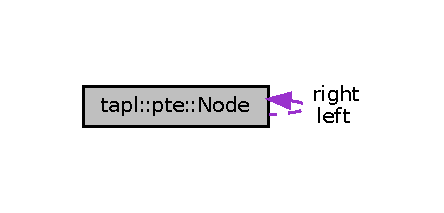
\includegraphics[width=213pt]{structtapl_1_1pte_1_1Node__coll__graph}
\end{center}
\end{figure}
\doxysubsection*{Public Member Functions}
\begin{DoxyCompactItemize}
\item 
\mbox{\hyperlink{structtapl_1_1pte_1_1Node_afec8c3ce63e2269d7602de2f22dc11c6}{Node}} (std\+::vector$<$ float $>$ arr, int set\+Id)
\end{DoxyCompactItemize}
\doxysubsection*{Data Fields}
\begin{DoxyCompactItemize}
\item 
std\+::vector$<$ float $>$ \mbox{\hyperlink{structtapl_1_1pte_1_1Node_a8b3448deee1ff9e0c9873b25ee83dd23}{point}}
\item 
int \mbox{\hyperlink{structtapl_1_1pte_1_1Node_a4141ba3367563df6be438c4344042b09}{id}}
\item 
\mbox{\hyperlink{structtapl_1_1pte_1_1Node}{Node}} $\ast$ \mbox{\hyperlink{structtapl_1_1pte_1_1Node_afaef86b1bf78932339871f61ad88535b}{left}}
\item 
\mbox{\hyperlink{structtapl_1_1pte_1_1Node}{Node}} $\ast$ \mbox{\hyperlink{structtapl_1_1pte_1_1Node_ab68a326fa1516aa082032dfd05065dd9}{right}}
\end{DoxyCompactItemize}


\doxysubsection{Detailed Description}


Definition at line 77 of file pt\+Engine.\+hpp.



\doxysubsection{Constructor \& Destructor Documentation}
\mbox{\Hypertarget{structtapl_1_1pte_1_1Node_afec8c3ce63e2269d7602de2f22dc11c6}\label{structtapl_1_1pte_1_1Node_afec8c3ce63e2269d7602de2f22dc11c6}} 
\index{tapl::pte::Node@{tapl::pte::Node}!Node@{Node}}
\index{Node@{Node}!tapl::pte::Node@{tapl::pte::Node}}
\doxysubsubsection{\texorpdfstring{Node()}{Node()}}
{\footnotesize\ttfamily tapl\+::pte\+::\+Node\+::\+Node (\begin{DoxyParamCaption}\item[{std\+::vector$<$ float $>$}]{arr,  }\item[{int}]{set\+Id }\end{DoxyParamCaption})\hspace{0.3cm}{\ttfamily [inline]}}



Definition at line 83 of file pt\+Engine.\+hpp.



\doxysubsection{Field Documentation}
\mbox{\Hypertarget{structtapl_1_1pte_1_1Node_a4141ba3367563df6be438c4344042b09}\label{structtapl_1_1pte_1_1Node_a4141ba3367563df6be438c4344042b09}} 
\index{tapl::pte::Node@{tapl::pte::Node}!id@{id}}
\index{id@{id}!tapl::pte::Node@{tapl::pte::Node}}
\doxysubsubsection{\texorpdfstring{id}{id}}
{\footnotesize\ttfamily int tapl\+::pte\+::\+Node\+::id}



Definition at line 79 of file pt\+Engine.\+hpp.

\mbox{\Hypertarget{structtapl_1_1pte_1_1Node_afaef86b1bf78932339871f61ad88535b}\label{structtapl_1_1pte_1_1Node_afaef86b1bf78932339871f61ad88535b}} 
\index{tapl::pte::Node@{tapl::pte::Node}!left@{left}}
\index{left@{left}!tapl::pte::Node@{tapl::pte::Node}}
\doxysubsubsection{\texorpdfstring{left}{left}}
{\footnotesize\ttfamily \mbox{\hyperlink{structtapl_1_1pte_1_1Node}{Node}}$\ast$ tapl\+::pte\+::\+Node\+::left}



Definition at line 80 of file pt\+Engine.\+hpp.

\mbox{\Hypertarget{structtapl_1_1pte_1_1Node_a8b3448deee1ff9e0c9873b25ee83dd23}\label{structtapl_1_1pte_1_1Node_a8b3448deee1ff9e0c9873b25ee83dd23}} 
\index{tapl::pte::Node@{tapl::pte::Node}!point@{point}}
\index{point@{point}!tapl::pte::Node@{tapl::pte::Node}}
\doxysubsubsection{\texorpdfstring{point}{point}}
{\footnotesize\ttfamily std\+::vector$<$float$>$ tapl\+::pte\+::\+Node\+::point}



Definition at line 78 of file pt\+Engine.\+hpp.

\mbox{\Hypertarget{structtapl_1_1pte_1_1Node_ab68a326fa1516aa082032dfd05065dd9}\label{structtapl_1_1pte_1_1Node_ab68a326fa1516aa082032dfd05065dd9}} 
\index{tapl::pte::Node@{tapl::pte::Node}!right@{right}}
\index{right@{right}!tapl::pte::Node@{tapl::pte::Node}}
\doxysubsubsection{\texorpdfstring{right}{right}}
{\footnotesize\ttfamily \mbox{\hyperlink{structtapl_1_1pte_1_1Node}{Node}}$\ast$ tapl\+::pte\+::\+Node\+::right}



Definition at line 81 of file pt\+Engine.\+hpp.



The documentation for this struct was generated from the following file\+:\begin{DoxyCompactItemize}
\item 
tapl/pte/\mbox{\hyperlink{ptEngine_8hpp}{pt\+Engine.\+hpp}}\end{DoxyCompactItemize}

\hypertarget{classtapl_1_1pte_1_1Plane}{}\doxysection{tapl\+::pte\+::Plane$<$ PointT $>$ Class Template Reference}
\label{classtapl_1_1pte_1_1Plane}\index{tapl::pte::Plane$<$ PointT $>$@{tapl::pte::Plane$<$ PointT $>$}}


{\ttfamily \#include $<$pt\+Engine.\+hpp$>$}

\doxysubsection*{Public Member Functions}
\begin{DoxyCompactItemize}
\item 
\mbox{\hyperlink{classtapl_1_1pte_1_1Plane_afab4f82143c003d0311b04c7d412d40c}{Plane}} ()
\item 
\mbox{\hyperlink{classtapl_1_1pte_1_1Plane_a9227e27649697d2d54f21f2cd8e4d6dd}{$\sim$\+Plane}} ()
\item 
std\+::vector$<$ float $>$ \mbox{\hyperlink{classtapl_1_1pte_1_1Plane_a3e0c52b8169fd9edf4c5bbb816432348}{fit\+S\+VD}} (std\+::vector$<$ float $>$ \&x, std\+::vector$<$ float $>$ \&y, std\+::vector$<$ float $>$ \&z)
\item 
std\+::vector$<$ float $>$ \mbox{\hyperlink{classtapl_1_1pte_1_1Plane_a1f943f3b0304c91e86a75a11579dee95}{fit\+LS}} (std\+::vector$<$ float $>$ \&x, std\+::vector$<$ float $>$ \&y, std\+::vector$<$ float $>$ \&z)
\item 
float \mbox{\hyperlink{classtapl_1_1pte_1_1Plane_af3adadd3b24d6c6a5750186e1828b26f}{dist\+To\+Point}} (std\+::vector$<$ float $>$ plane\+\_\+coeffs, PointT point)
\item 
std\+::unordered\+\_\+set$<$ int $>$ \mbox{\hyperlink{classtapl_1_1pte_1_1Plane_ad56c96d9b115a8a482e851c8139feb97}{Ransac}} (typename pcl\+::\+Point\+Cloud$<$ PointT $>$\+::Ptr cloud, int max\+Iterations, float distance\+To\+Plane)
\end{DoxyCompactItemize}


\doxysubsection{Detailed Description}
\subsubsection*{template$<$typename PointT$>$\newline
class tapl\+::pte\+::\+Plane$<$ Point\+T $>$}



Definition at line 55 of file pt\+Engine.\+hpp.



\doxysubsection{Constructor \& Destructor Documentation}
\mbox{\Hypertarget{classtapl_1_1pte_1_1Plane_afab4f82143c003d0311b04c7d412d40c}\label{classtapl_1_1pte_1_1Plane_afab4f82143c003d0311b04c7d412d40c}} 
\index{tapl::pte::Plane$<$ PointT $>$@{tapl::pte::Plane$<$ PointT $>$}!Plane@{Plane}}
\index{Plane@{Plane}!tapl::pte::Plane$<$ PointT $>$@{tapl::pte::Plane$<$ PointT $>$}}
\doxysubsubsection{\texorpdfstring{Plane()}{Plane()}}
{\footnotesize\ttfamily template$<$typename PointT $>$ \\
\mbox{\hyperlink{classtapl_1_1pte_1_1Plane}{tapl\+::pte\+::\+Plane}}$<$ PointT $>$\+::\mbox{\hyperlink{classtapl_1_1pte_1_1Plane}{Plane}}}



Definition at line 173 of file pt\+Engine.\+cpp.

\mbox{\Hypertarget{classtapl_1_1pte_1_1Plane_a9227e27649697d2d54f21f2cd8e4d6dd}\label{classtapl_1_1pte_1_1Plane_a9227e27649697d2d54f21f2cd8e4d6dd}} 
\index{tapl::pte::Plane$<$ PointT $>$@{tapl::pte::Plane$<$ PointT $>$}!````~Plane@{$\sim$Plane}}
\index{````~Plane@{$\sim$Plane}!tapl::pte::Plane$<$ PointT $>$@{tapl::pte::Plane$<$ PointT $>$}}
\doxysubsubsection{\texorpdfstring{$\sim$Plane()}{~Plane()}}
{\footnotesize\ttfamily template$<$typename PointT $>$ \\
\mbox{\hyperlink{classtapl_1_1pte_1_1Plane}{tapl\+::pte\+::\+Plane}}$<$ PointT $>$\+::$\sim$\mbox{\hyperlink{classtapl_1_1pte_1_1Plane}{Plane}}}



Definition at line 177 of file pt\+Engine.\+cpp.



\doxysubsection{Member Function Documentation}
\mbox{\Hypertarget{classtapl_1_1pte_1_1Plane_af3adadd3b24d6c6a5750186e1828b26f}\label{classtapl_1_1pte_1_1Plane_af3adadd3b24d6c6a5750186e1828b26f}} 
\index{tapl::pte::Plane$<$ PointT $>$@{tapl::pte::Plane$<$ PointT $>$}!distToPoint@{distToPoint}}
\index{distToPoint@{distToPoint}!tapl::pte::Plane$<$ PointT $>$@{tapl::pte::Plane$<$ PointT $>$}}
\doxysubsubsection{\texorpdfstring{distToPoint()}{distToPoint()}}
{\footnotesize\ttfamily template$<$typename PointT $>$ \\
float \mbox{\hyperlink{classtapl_1_1pte_1_1Plane}{tapl\+::pte\+::\+Plane}}$<$ PointT $>$\+::dist\+To\+Point (\begin{DoxyParamCaption}\item[{std\+::vector$<$ float $>$}]{plane\+\_\+coeffs,  }\item[{PointT}]{point }\end{DoxyParamCaption})}



Definition at line 261 of file pt\+Engine.\+cpp.

\mbox{\Hypertarget{classtapl_1_1pte_1_1Plane_a1f943f3b0304c91e86a75a11579dee95}\label{classtapl_1_1pte_1_1Plane_a1f943f3b0304c91e86a75a11579dee95}} 
\index{tapl::pte::Plane$<$ PointT $>$@{tapl::pte::Plane$<$ PointT $>$}!fitLS@{fitLS}}
\index{fitLS@{fitLS}!tapl::pte::Plane$<$ PointT $>$@{tapl::pte::Plane$<$ PointT $>$}}
\doxysubsubsection{\texorpdfstring{fitLS()}{fitLS()}}
{\footnotesize\ttfamily template$<$typename PointT $>$ \\
std\+::vector$<$ float $>$ \mbox{\hyperlink{classtapl_1_1pte_1_1Plane}{tapl\+::pte\+::\+Plane}}$<$ PointT $>$\+::fit\+LS (\begin{DoxyParamCaption}\item[{std\+::vector$<$ float $>$ \&}]{x,  }\item[{std\+::vector$<$ float $>$ \&}]{y,  }\item[{std\+::vector$<$ float $>$ \&}]{z }\end{DoxyParamCaption})}



Definition at line 215 of file pt\+Engine.\+cpp.

\mbox{\Hypertarget{classtapl_1_1pte_1_1Plane_a3e0c52b8169fd9edf4c5bbb816432348}\label{classtapl_1_1pte_1_1Plane_a3e0c52b8169fd9edf4c5bbb816432348}} 
\index{tapl::pte::Plane$<$ PointT $>$@{tapl::pte::Plane$<$ PointT $>$}!fitSVD@{fitSVD}}
\index{fitSVD@{fitSVD}!tapl::pte::Plane$<$ PointT $>$@{tapl::pte::Plane$<$ PointT $>$}}
\doxysubsubsection{\texorpdfstring{fitSVD()}{fitSVD()}}
{\footnotesize\ttfamily template$<$typename PointT $>$ \\
std\+::vector$<$ float $>$ \mbox{\hyperlink{classtapl_1_1pte_1_1Plane}{tapl\+::pte\+::\+Plane}}$<$ PointT $>$\+::fit\+S\+VD (\begin{DoxyParamCaption}\item[{std\+::vector$<$ float $>$ \&}]{x,  }\item[{std\+::vector$<$ float $>$ \&}]{y,  }\item[{std\+::vector$<$ float $>$ \&}]{z }\end{DoxyParamCaption})}



Definition at line 180 of file pt\+Engine.\+cpp.

\mbox{\Hypertarget{classtapl_1_1pte_1_1Plane_ad56c96d9b115a8a482e851c8139feb97}\label{classtapl_1_1pte_1_1Plane_ad56c96d9b115a8a482e851c8139feb97}} 
\index{tapl::pte::Plane$<$ PointT $>$@{tapl::pte::Plane$<$ PointT $>$}!Ransac@{Ransac}}
\index{Ransac@{Ransac}!tapl::pte::Plane$<$ PointT $>$@{tapl::pte::Plane$<$ PointT $>$}}
\doxysubsubsection{\texorpdfstring{Ransac()}{Ransac()}}
{\footnotesize\ttfamily template$<$typename PointT $>$ \\
std\+::unordered\+\_\+set$<$ int $>$ \mbox{\hyperlink{classtapl_1_1pte_1_1Plane}{tapl\+::pte\+::\+Plane}}$<$ PointT $>$\+::Ransac (\begin{DoxyParamCaption}\item[{typename pcl\+::\+Point\+Cloud$<$ PointT $>$\+::Ptr}]{cloud,  }\item[{int}]{max\+Iterations,  }\item[{float}]{distance\+To\+Plane }\end{DoxyParamCaption})}



Definition at line 270 of file pt\+Engine.\+cpp.

Here is the caller graph for this function\+:
\nopagebreak
\begin{figure}[H]
\begin{center}
\leavevmode
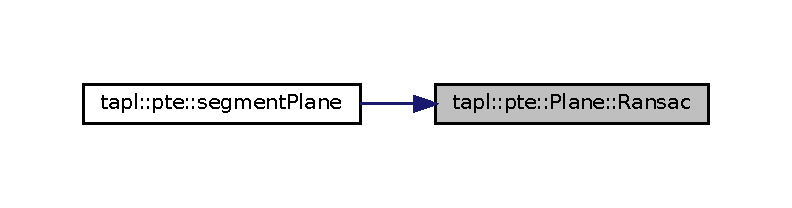
\includegraphics[width=350pt]{classtapl_1_1pte_1_1Plane_ad56c96d9b115a8a482e851c8139feb97_icgraph}
\end{center}
\end{figure}


The documentation for this class was generated from the following files\+:\begin{DoxyCompactItemize}
\item 
tapl/pte/\mbox{\hyperlink{ptEngine_8hpp}{pt\+Engine.\+hpp}}\item 
tapl/pte/\mbox{\hyperlink{ptEngine_8cpp}{pt\+Engine.\+cpp}}\end{DoxyCompactItemize}

\hypertarget{structtapl_1_1Pose6dof}{}\section{tapl\+:\+:Pose6dof Struct Reference}
\label{structtapl_1_1Pose6dof}\index{tapl\+::\+Pose6dof@{tapl\+::\+Pose6dof}}


6-\/\+D\+OF Camera Pose  




{\ttfamily \#include $<$tapl\+Types.\+hpp$>$}

\subsection*{Public Member Functions}
\begin{DoxyCompactItemize}
\item 
\hyperlink{structtapl_1_1Pose6dof_a48869500ca9d0fe0e2936132eaec566e}{Pose6dof} ()
\end{DoxyCompactItemize}
\subsection*{Data Fields}
\begin{DoxyCompactItemize}
\item 
cv\+::\+Mat \hyperlink{structtapl_1_1Pose6dof_a0ff2d0d3cb7c4d1cb83ffd8545dbbfa0}{R}
\item 
cv\+::\+Mat \hyperlink{structtapl_1_1Pose6dof_aaac0151b90bd28d462e400e5b5dbefcb}{t}
\item 
cv\+::\+Mat \hyperlink{structtapl_1_1Pose6dof_a2cc91e38bb0080f6e1760902613cc093}{P}
\item 
cv\+::\+Mat \hyperlink{structtapl_1_1Pose6dof_afa5dd6803d0f682139676e27ff20b9d2}{euler}
\end{DoxyCompactItemize}


\subsection{Detailed Description}
6-\/\+D\+OF Camera Pose 

Definition at line 38 of file tapl\+Types.\+hpp.



\subsection{Constructor \& Destructor Documentation}
\index{tapl\+::\+Pose6dof@{tapl\+::\+Pose6dof}!Pose6dof@{Pose6dof}}
\index{Pose6dof@{Pose6dof}!tapl\+::\+Pose6dof@{tapl\+::\+Pose6dof}}
\subsubsection[{\texorpdfstring{Pose6dof()}{Pose6dof()}}]{\setlength{\rightskip}{0pt plus 5cm}tapl\+::\+Pose6dof\+::\+Pose6dof (
\begin{DoxyParamCaption}
{}
\end{DoxyParamCaption}
)\hspace{0.3cm}{\ttfamily [inline]}}\hypertarget{structtapl_1_1Pose6dof_a48869500ca9d0fe0e2936132eaec566e}{}\label{structtapl_1_1Pose6dof_a48869500ca9d0fe0e2936132eaec566e}


Definition at line 46 of file tapl\+Types.\+hpp.



\subsection{Field Documentation}
\index{tapl\+::\+Pose6dof@{tapl\+::\+Pose6dof}!euler@{euler}}
\index{euler@{euler}!tapl\+::\+Pose6dof@{tapl\+::\+Pose6dof}}
\subsubsection[{\texorpdfstring{euler}{euler}}]{\setlength{\rightskip}{0pt plus 5cm}cv\+::\+Mat tapl\+::\+Pose6dof\+::euler}\hypertarget{structtapl_1_1Pose6dof_afa5dd6803d0f682139676e27ff20b9d2}{}\label{structtapl_1_1Pose6dof_afa5dd6803d0f682139676e27ff20b9d2}
roll, pitch, yaw in radians 

Definition at line 43 of file tapl\+Types.\+hpp.

\index{tapl\+::\+Pose6dof@{tapl\+::\+Pose6dof}!P@{P}}
\index{P@{P}!tapl\+::\+Pose6dof@{tapl\+::\+Pose6dof}}
\subsubsection[{\texorpdfstring{P}{P}}]{\setlength{\rightskip}{0pt plus 5cm}cv\+::\+Mat tapl\+::\+Pose6dof\+::P}\hypertarget{structtapl_1_1Pose6dof_a2cc91e38bb0080f6e1760902613cc093}{}\label{structtapl_1_1Pose6dof_a2cc91e38bb0080f6e1760902613cc093}
4x4 projection matrix which combines both rotation and translation matrix 

Definition at line 41 of file tapl\+Types.\+hpp.

\index{tapl\+::\+Pose6dof@{tapl\+::\+Pose6dof}!R@{R}}
\index{R@{R}!tapl\+::\+Pose6dof@{tapl\+::\+Pose6dof}}
\subsubsection[{\texorpdfstring{R}{R}}]{\setlength{\rightskip}{0pt plus 5cm}cv\+::\+Mat tapl\+::\+Pose6dof\+::R}\hypertarget{structtapl_1_1Pose6dof_a0ff2d0d3cb7c4d1cb83ffd8545dbbfa0}{}\label{structtapl_1_1Pose6dof_a0ff2d0d3cb7c4d1cb83ffd8545dbbfa0}
3x3 rotation matrix 

Definition at line 39 of file tapl\+Types.\+hpp.

\index{tapl\+::\+Pose6dof@{tapl\+::\+Pose6dof}!t@{t}}
\index{t@{t}!tapl\+::\+Pose6dof@{tapl\+::\+Pose6dof}}
\subsubsection[{\texorpdfstring{t}{t}}]{\setlength{\rightskip}{0pt plus 5cm}cv\+::\+Mat tapl\+::\+Pose6dof\+::t}\hypertarget{structtapl_1_1Pose6dof_aaac0151b90bd28d462e400e5b5dbefcb}{}\label{structtapl_1_1Pose6dof_aaac0151b90bd28d462e400e5b5dbefcb}
1x3 translation vector 

Definition at line 40 of file tapl\+Types.\+hpp.



The documentation for this struct was generated from the following file\+:\begin{DoxyCompactItemize}
\item 
tapl/\hyperlink{taplTypes_8hpp}{tapl\+Types.\+hpp}\end{DoxyCompactItemize}

\hypertarget{classtapl_1_1RingBuffer}{}\doxysection{tapl\+::Ring\+Buffer$<$ T $>$ Class Template Reference}
\label{classtapl_1_1RingBuffer}\index{tapl::RingBuffer$<$ T $>$@{tapl::RingBuffer$<$ T $>$}}


Ring Buffer.  




{\ttfamily \#include $<$ring\+Buffer.\+hpp$>$}

\doxysubsection*{Public Member Functions}
\begin{DoxyCompactItemize}
\item 
\mbox{\hyperlink{classtapl_1_1RingBuffer_ad164e0fc13d245411c356ad687dc504a}{Ring\+Buffer}} (uint16\+\_\+t max\+\_\+size)
\item 
\mbox{\hyperlink{classtapl_1_1RingBuffer_a8e9cc0e12555c499b95a9a6e7943a4d7}{$\sim$\+Ring\+Buffer}} ()
\item 
uint16\+\_\+t \mbox{\hyperlink{classtapl_1_1RingBuffer_a5dfe06176646eeacfb89c464b15815ff}{get\+Size}} ()
\item 
void \mbox{\hyperlink{classtapl_1_1RingBuffer_aa2ab87a6e5b95daf4b9f59e35c24396d}{push}} (T const data)
\item 
T \mbox{\hyperlink{classtapl_1_1RingBuffer_aad957e002e355729e1ef044538ccf110}{pop}} ()
\item 
T \mbox{\hyperlink{classtapl_1_1RingBuffer_a86bd7fbf2c52259184c4e84feaae78d3}{get}} (uint16\+\_\+t index)
\item 
T $\ast$ \mbox{\hyperlink{classtapl_1_1RingBuffer_ae1c8614abf72c558c244c87b8ced7bf7}{get\+\_\+ptr}} (uint16\+\_\+t index)
\end{DoxyCompactItemize}


\doxysubsection{Detailed Description}
\subsubsection*{template$<$typename T$>$\newline
class tapl\+::\+Ring\+Buffer$<$ T $>$}

Ring Buffer. 

Definition at line 19 of file ring\+Buffer.\+hpp.



\doxysubsection{Constructor \& Destructor Documentation}
\mbox{\Hypertarget{classtapl_1_1RingBuffer_ad164e0fc13d245411c356ad687dc504a}\label{classtapl_1_1RingBuffer_ad164e0fc13d245411c356ad687dc504a}} 
\index{tapl::RingBuffer$<$ T $>$@{tapl::RingBuffer$<$ T $>$}!RingBuffer@{RingBuffer}}
\index{RingBuffer@{RingBuffer}!tapl::RingBuffer$<$ T $>$@{tapl::RingBuffer$<$ T $>$}}
\doxysubsubsection{\texorpdfstring{RingBuffer()}{RingBuffer()}}
{\footnotesize\ttfamily template$<$typename T $>$ \\
\mbox{\hyperlink{classtapl_1_1RingBuffer}{tapl\+::\+Ring\+Buffer}}$<$ T $>$\+::\mbox{\hyperlink{classtapl_1_1RingBuffer}{Ring\+Buffer}} (\begin{DoxyParamCaption}\item[{uint16\+\_\+t}]{max\+\_\+size }\end{DoxyParamCaption})\hspace{0.3cm}{\ttfamily [inline]}}



Definition at line 34 of file ring\+Buffer.\+hpp.

\mbox{\Hypertarget{classtapl_1_1RingBuffer_a8e9cc0e12555c499b95a9a6e7943a4d7}\label{classtapl_1_1RingBuffer_a8e9cc0e12555c499b95a9a6e7943a4d7}} 
\index{tapl::RingBuffer$<$ T $>$@{tapl::RingBuffer$<$ T $>$}!````~RingBuffer@{$\sim$RingBuffer}}
\index{````~RingBuffer@{$\sim$RingBuffer}!tapl::RingBuffer$<$ T $>$@{tapl::RingBuffer$<$ T $>$}}
\doxysubsubsection{\texorpdfstring{$\sim$RingBuffer()}{~RingBuffer()}}
{\footnotesize\ttfamily template$<$typename T $>$ \\
\mbox{\hyperlink{classtapl_1_1RingBuffer}{tapl\+::\+Ring\+Buffer}}$<$ T $>$\+::$\sim$\mbox{\hyperlink{classtapl_1_1RingBuffer}{Ring\+Buffer}} (\begin{DoxyParamCaption}{ }\end{DoxyParamCaption})\hspace{0.3cm}{\ttfamily [inline]}}



Definition at line 51 of file ring\+Buffer.\+hpp.



\doxysubsection{Member Function Documentation}
\mbox{\Hypertarget{classtapl_1_1RingBuffer_a86bd7fbf2c52259184c4e84feaae78d3}\label{classtapl_1_1RingBuffer_a86bd7fbf2c52259184c4e84feaae78d3}} 
\index{tapl::RingBuffer$<$ T $>$@{tapl::RingBuffer$<$ T $>$}!get@{get}}
\index{get@{get}!tapl::RingBuffer$<$ T $>$@{tapl::RingBuffer$<$ T $>$}}
\doxysubsubsection{\texorpdfstring{get()}{get()}}
{\footnotesize\ttfamily template$<$typename T $>$ \\
T \mbox{\hyperlink{classtapl_1_1RingBuffer}{tapl\+::\+Ring\+Buffer}}$<$ T $>$\+::get (\begin{DoxyParamCaption}\item[{uint16\+\_\+t}]{index }\end{DoxyParamCaption})\hspace{0.3cm}{\ttfamily [inline]}}



Definition at line 96 of file ring\+Buffer.\+hpp.

\mbox{\Hypertarget{classtapl_1_1RingBuffer_ae1c8614abf72c558c244c87b8ced7bf7}\label{classtapl_1_1RingBuffer_ae1c8614abf72c558c244c87b8ced7bf7}} 
\index{tapl::RingBuffer$<$ T $>$@{tapl::RingBuffer$<$ T $>$}!get\_ptr@{get\_ptr}}
\index{get\_ptr@{get\_ptr}!tapl::RingBuffer$<$ T $>$@{tapl::RingBuffer$<$ T $>$}}
\doxysubsubsection{\texorpdfstring{get\_ptr()}{get\_ptr()}}
{\footnotesize\ttfamily template$<$typename T $>$ \\
T$\ast$ \mbox{\hyperlink{classtapl_1_1RingBuffer}{tapl\+::\+Ring\+Buffer}}$<$ T $>$\+::get\+\_\+ptr (\begin{DoxyParamCaption}\item[{uint16\+\_\+t}]{index }\end{DoxyParamCaption})\hspace{0.3cm}{\ttfamily [inline]}}



Definition at line 116 of file ring\+Buffer.\+hpp.

\mbox{\Hypertarget{classtapl_1_1RingBuffer_a5dfe06176646eeacfb89c464b15815ff}\label{classtapl_1_1RingBuffer_a5dfe06176646eeacfb89c464b15815ff}} 
\index{tapl::RingBuffer$<$ T $>$@{tapl::RingBuffer$<$ T $>$}!getSize@{getSize}}
\index{getSize@{getSize}!tapl::RingBuffer$<$ T $>$@{tapl::RingBuffer$<$ T $>$}}
\doxysubsubsection{\texorpdfstring{getSize()}{getSize()}}
{\footnotesize\ttfamily template$<$typename T $>$ \\
uint16\+\_\+t \mbox{\hyperlink{classtapl_1_1RingBuffer}{tapl\+::\+Ring\+Buffer}}$<$ T $>$\+::get\+Size (\begin{DoxyParamCaption}{ }\end{DoxyParamCaption})\hspace{0.3cm}{\ttfamily [inline]}}



Definition at line 54 of file ring\+Buffer.\+hpp.

\mbox{\Hypertarget{classtapl_1_1RingBuffer_aad957e002e355729e1ef044538ccf110}\label{classtapl_1_1RingBuffer_aad957e002e355729e1ef044538ccf110}} 
\index{tapl::RingBuffer$<$ T $>$@{tapl::RingBuffer$<$ T $>$}!pop@{pop}}
\index{pop@{pop}!tapl::RingBuffer$<$ T $>$@{tapl::RingBuffer$<$ T $>$}}
\doxysubsubsection{\texorpdfstring{pop()}{pop()}}
{\footnotesize\ttfamily template$<$typename T $>$ \\
T \mbox{\hyperlink{classtapl_1_1RingBuffer}{tapl\+::\+Ring\+Buffer}}$<$ T $>$\+::pop (\begin{DoxyParamCaption}{ }\end{DoxyParamCaption})\hspace{0.3cm}{\ttfamily [inline]}}



Definition at line 78 of file ring\+Buffer.\+hpp.

\mbox{\Hypertarget{classtapl_1_1RingBuffer_aa2ab87a6e5b95daf4b9f59e35c24396d}\label{classtapl_1_1RingBuffer_aa2ab87a6e5b95daf4b9f59e35c24396d}} 
\index{tapl::RingBuffer$<$ T $>$@{tapl::RingBuffer$<$ T $>$}!push@{push}}
\index{push@{push}!tapl::RingBuffer$<$ T $>$@{tapl::RingBuffer$<$ T $>$}}
\doxysubsubsection{\texorpdfstring{push()}{push()}}
{\footnotesize\ttfamily template$<$typename T $>$ \\
void \mbox{\hyperlink{classtapl_1_1RingBuffer}{tapl\+::\+Ring\+Buffer}}$<$ T $>$\+::push (\begin{DoxyParamCaption}\item[{T const}]{data }\end{DoxyParamCaption})\hspace{0.3cm}{\ttfamily [inline]}}



Definition at line 59 of file ring\+Buffer.\+hpp.



The documentation for this class was generated from the following file\+:\begin{DoxyCompactItemize}
\item 
tapl/common/\mbox{\hyperlink{ringBuffer_8hpp}{ring\+Buffer.\+hpp}}\end{DoxyCompactItemize}

\hypertarget{classtapl_1_1viz_1_1Visualizer}{}\doxysection{tapl\+::viz\+::Visualizer Class Reference}
\label{classtapl_1_1viz_1_1Visualizer}\index{tapl::viz::Visualizer@{tapl::viz::Visualizer}}


Implementation of the visualizer class.  




{\ttfamily \#include $<$visualization.\+hpp$>$}

\doxysubsection*{Public Member Functions}
\begin{DoxyCompactItemize}
\item 
\mbox{\hyperlink{classtapl_1_1viz_1_1Visualizer_a56215eefb4712acf78a922485d844f50}{Visualizer}} (float r=0., float g=0., float b=0., \mbox{\hyperlink{namespacetapl_1_1viz_a99e496921984514dbc7bcef809f50150}{Camera\+Angle}} cam\+Angle=\mbox{\hyperlink{namespacetapl_1_1viz_a99e496921984514dbc7bcef809f50150a9aa35eea1fe8f4b45a0b02a8b5048cfa}{Top\+Down}}, float distance=20.\+0)
\item 
\mbox{\hyperlink{classtapl_1_1viz_1_1Visualizer_a47473d1bffdf617379d718f1c2ed5930}{$\sim$\+Visualizer}} ()
\item 
{\footnotesize template$<$typename PointT $>$ }\\void \mbox{\hyperlink{classtapl_1_1viz_1_1Visualizer_a1ffe49d8e3b2693b0c0a4ccd10edac9d}{render\+Sphere}} (const PointT \&pt, float radius, const std\+::string \&id)
\begin{DoxyCompactList}\small\item\em This function is used to render a sphere on the visualizer. \end{DoxyCompactList}\item 
{\footnotesize template$<$typename PointT $>$ }\\void \mbox{\hyperlink{classtapl_1_1viz_1_1Visualizer_acca33adaa4aeaeca6f393dee319b36b8}{render\+Sphere}} (const PointT \&pt, float radius, float r, float g, float b, const std\+::string \&id)
\begin{DoxyCompactList}\small\item\em This function is used to render a sphere on the visualizer. \end{DoxyCompactList}\item 
{\footnotesize template$<$typename PointT $>$ }\\void \mbox{\hyperlink{classtapl_1_1viz_1_1Visualizer_a44e1d90914fa8129f4e4a26b4ad67718}{render\+Line}} (const PointT \&pt1, const PointT \&pt2, const std\+::string \&id)
\begin{DoxyCompactList}\small\item\em This function is used to render a line on the visualizer. \end{DoxyCompactList}\item 
{\footnotesize template$<$typename PointT $>$ }\\void \mbox{\hyperlink{classtapl_1_1viz_1_1Visualizer_a23442f9881a361b9ff0aff3b18f1eea0}{render\+Line}} (const PointT \&pt1, const PointT \&pt2, float r, float g, float b, const std\+::string \&id)
\begin{DoxyCompactList}\small\item\em This function is used to render a line on the visualizer. \end{DoxyCompactList}\item 
void \mbox{\hyperlink{classtapl_1_1viz_1_1Visualizer_a22497fa3f1d2738c1b0a3f963a7c43dd}{render\+Pose}} (float scale, float x, float y, float z, const std\+::string \&id=\char`\"{}pose\char`\"{})
\begin{DoxyCompactList}\small\item\em Adds 3-\/D\+OF pose. \end{DoxyCompactList}\item 
void \mbox{\hyperlink{classtapl_1_1viz_1_1Visualizer_ae24ff2fab8c5107d931cd175abd916ef}{render\+Pose}} (float scale, const Eigen\+::\+Affine3f \&pose, const std\+::string \&id=\char`\"{}pose\char`\"{})
\begin{DoxyCompactList}\small\item\em Adds 6-\/D\+OF pose defined by a 4x4 transformation matrix. \end{DoxyCompactList}\item 
{\footnotesize template$<$typename PointT $>$ }\\void \mbox{\hyperlink{classtapl_1_1viz_1_1Visualizer_a5c6a85b27b5042f09b0e7034ee73209c}{render\+Point\+Cloud}} (const typename pcl\+::\+Point\+Cloud$<$ PointT $>$\+::Const\+Ptr \&cloud, float ptsize=1.\+0, float r=1.\+0, float g=0.\+0, float b=0.\+0, const std\+::string \&id=\char`\"{}cloud\char`\"{})
\begin{DoxyCompactList}\small\item\em Render a point-\/cloud. \end{DoxyCompactList}\item 
void \mbox{\hyperlink{classtapl_1_1viz_1_1Visualizer_a3915205a2348669a0399b3f1a2e8551c}{render\+Bbox3d}} (const \mbox{\hyperlink{structtapl_1_1BBox3d}{B\+Box3d}} \&box, float r=1.\+0, float g=0.\+0, float b=0.\+0, float opacity=0.\+5, const std\+::string \&id=\char`\"{}bbox\char`\"{})
\begin{DoxyCompactList}\small\item\em Render a 3d bounding-\/box. \end{DoxyCompactList}\item 
void \mbox{\hyperlink{classtapl_1_1viz_1_1Visualizer_a8ec08b4e37523fb75731b58748224035}{render\+Scene}} (int time=1)
\begin{DoxyCompactList}\small\item\em Render the scene once. \end{DoxyCompactList}\item 
void \mbox{\hyperlink{classtapl_1_1viz_1_1Visualizer_aed14efd9e578a4b6013b9745e07acea1}{render\+Scene\+And\+Hold}} ()
\begin{DoxyCompactList}\small\item\em Render the scene and hold. \end{DoxyCompactList}\item 
void \mbox{\hyperlink{classtapl_1_1viz_1_1Visualizer_a912479d651c5a9bcd5a24b77025f10c0}{clear\+Scene}} ()
\begin{DoxyCompactList}\small\item\em Clear the scene. \end{DoxyCompactList}\end{DoxyCompactItemize}


\doxysubsection{Detailed Description}
Implementation of the visualizer class. 

Definition at line 27 of file visualization.\+hpp.



\doxysubsection{Constructor \& Destructor Documentation}
\mbox{\Hypertarget{classtapl_1_1viz_1_1Visualizer_a56215eefb4712acf78a922485d844f50}\label{classtapl_1_1viz_1_1Visualizer_a56215eefb4712acf78a922485d844f50}} 
\index{tapl::viz::Visualizer@{tapl::viz::Visualizer}!Visualizer@{Visualizer}}
\index{Visualizer@{Visualizer}!tapl::viz::Visualizer@{tapl::viz::Visualizer}}
\doxysubsubsection{\texorpdfstring{Visualizer()}{Visualizer()}}
{\footnotesize\ttfamily tapl\+::viz\+::\+Visualizer\+::\+Visualizer (\begin{DoxyParamCaption}\item[{float}]{r = {\ttfamily 0.},  }\item[{float}]{g = {\ttfamily 0.},  }\item[{float}]{b = {\ttfamily 0.},  }\item[{\mbox{\hyperlink{namespacetapl_1_1viz_a99e496921984514dbc7bcef809f50150}{Camera\+Angle}}}]{cam\+Angle = {\ttfamily \mbox{\hyperlink{namespacetapl_1_1viz_a99e496921984514dbc7bcef809f50150a9aa35eea1fe8f4b45a0b02a8b5048cfa}{Top\+Down}}},  }\item[{float}]{distance = {\ttfamily 20.0} }\end{DoxyParamCaption})\hspace{0.3cm}{\ttfamily [inline]}}



Definition at line 34 of file visualization.\+hpp.

\mbox{\Hypertarget{classtapl_1_1viz_1_1Visualizer_a47473d1bffdf617379d718f1c2ed5930}\label{classtapl_1_1viz_1_1Visualizer_a47473d1bffdf617379d718f1c2ed5930}} 
\index{tapl::viz::Visualizer@{tapl::viz::Visualizer}!````~Visualizer@{$\sim$Visualizer}}
\index{````~Visualizer@{$\sim$Visualizer}!tapl::viz::Visualizer@{tapl::viz::Visualizer}}
\doxysubsubsection{\texorpdfstring{$\sim$Visualizer()}{~Visualizer()}}
{\footnotesize\ttfamily tapl\+::viz\+::\+Visualizer\+::$\sim$\+Visualizer (\begin{DoxyParamCaption}{ }\end{DoxyParamCaption})\hspace{0.3cm}{\ttfamily [inline]}}



Definition at line 50 of file visualization.\+hpp.



\doxysubsection{Member Function Documentation}
\mbox{\Hypertarget{classtapl_1_1viz_1_1Visualizer_a912479d651c5a9bcd5a24b77025f10c0}\label{classtapl_1_1viz_1_1Visualizer_a912479d651c5a9bcd5a24b77025f10c0}} 
\index{tapl::viz::Visualizer@{tapl::viz::Visualizer}!clearScene@{clearScene}}
\index{clearScene@{clearScene}!tapl::viz::Visualizer@{tapl::viz::Visualizer}}
\doxysubsubsection{\texorpdfstring{clearScene()}{clearScene()}}
{\footnotesize\ttfamily void tapl\+::viz\+::\+Visualizer\+::clear\+Scene (\begin{DoxyParamCaption}{ }\end{DoxyParamCaption})\hspace{0.3cm}{\ttfamily [inline]}}



Clear the scene. 



Definition at line 217 of file visualization.\+hpp.

\mbox{\Hypertarget{classtapl_1_1viz_1_1Visualizer_a3915205a2348669a0399b3f1a2e8551c}\label{classtapl_1_1viz_1_1Visualizer_a3915205a2348669a0399b3f1a2e8551c}} 
\index{tapl::viz::Visualizer@{tapl::viz::Visualizer}!renderBbox3d@{renderBbox3d}}
\index{renderBbox3d@{renderBbox3d}!tapl::viz::Visualizer@{tapl::viz::Visualizer}}
\doxysubsubsection{\texorpdfstring{renderBbox3d()}{renderBbox3d()}}
{\footnotesize\ttfamily void tapl\+::viz\+::\+Visualizer\+::render\+Bbox3d (\begin{DoxyParamCaption}\item[{const \mbox{\hyperlink{structtapl_1_1BBox3d}{B\+Box3d}} \&}]{box,  }\item[{float}]{r = {\ttfamily 1.0},  }\item[{float}]{g = {\ttfamily 0.0},  }\item[{float}]{b = {\ttfamily 0.0},  }\item[{float}]{opacity = {\ttfamily 0.5},  }\item[{const std\+::string \&}]{id = {\ttfamily \char`\"{}bbox\char`\"{}} }\end{DoxyParamCaption})\hspace{0.3cm}{\ttfamily [inline]}}



Render a 3d bounding-\/box. 


\begin{DoxyParams}[1]{Parameters}
\mbox{\texttt{ in}}  & {\em box} & 3D Bounding-\/\+Box \\
\hline
\mbox{\texttt{ in}}  & {\em r} & specifies red in rgb colorspace for the color of sphere in range of \mbox{[}0.\+0, 1.\+0\mbox{]} \\
\hline
\mbox{\texttt{ in}}  & {\em g} & specifies green in rgb colorspace for the color of sphere in range of \mbox{[}0.\+0, 1.\+0\mbox{]} \\
\hline
\mbox{\texttt{ in}}  & {\em b} & specifies blue in rgb colorspace for the color of sphere in range of \mbox{[}0.\+0, 1.\+0\mbox{]} \\
\hline
\mbox{\texttt{ in}}  & {\em opacity} & opacity of the bounding box in range of \mbox{[}0.\+0, 1.\+0\mbox{]} \\
\hline
\mbox{\texttt{ in}}  & {\em id} & the bounding-\/box object id (default\+: bbox) \\
\hline
\end{DoxyParams}


Definition at line 177 of file visualization.\+hpp.

\mbox{\Hypertarget{classtapl_1_1viz_1_1Visualizer_a44e1d90914fa8129f4e4a26b4ad67718}\label{classtapl_1_1viz_1_1Visualizer_a44e1d90914fa8129f4e4a26b4ad67718}} 
\index{tapl::viz::Visualizer@{tapl::viz::Visualizer}!renderLine@{renderLine}}
\index{renderLine@{renderLine}!tapl::viz::Visualizer@{tapl::viz::Visualizer}}
\doxysubsubsection{\texorpdfstring{renderLine()}{renderLine()}\hspace{0.1cm}{\footnotesize\ttfamily [1/2]}}
{\footnotesize\ttfamily template$<$typename PointT $>$ \\
void tapl\+::viz\+::\+Visualizer\+::render\+Line (\begin{DoxyParamCaption}\item[{const PointT \&}]{pt1,  }\item[{const PointT \&}]{pt2,  }\item[{const std\+::string \&}]{id }\end{DoxyParamCaption})\hspace{0.3cm}{\ttfamily [inline]}}



This function is used to render a line on the visualizer. 


\begin{DoxyParams}[1]{Parameters}
\mbox{\texttt{ in}}  & {\em pt1} & start point of the line \\
\hline
\mbox{\texttt{ in}}  & {\em pt2} & end point of the line \\
\hline
\mbox{\texttt{ in}}  & {\em id} & a unique id for this line \\
\hline
\end{DoxyParams}


Definition at line 92 of file visualization.\+hpp.

\mbox{\Hypertarget{classtapl_1_1viz_1_1Visualizer_a23442f9881a361b9ff0aff3b18f1eea0}\label{classtapl_1_1viz_1_1Visualizer_a23442f9881a361b9ff0aff3b18f1eea0}} 
\index{tapl::viz::Visualizer@{tapl::viz::Visualizer}!renderLine@{renderLine}}
\index{renderLine@{renderLine}!tapl::viz::Visualizer@{tapl::viz::Visualizer}}
\doxysubsubsection{\texorpdfstring{renderLine()}{renderLine()}\hspace{0.1cm}{\footnotesize\ttfamily [2/2]}}
{\footnotesize\ttfamily template$<$typename PointT $>$ \\
void tapl\+::viz\+::\+Visualizer\+::render\+Line (\begin{DoxyParamCaption}\item[{const PointT \&}]{pt1,  }\item[{const PointT \&}]{pt2,  }\item[{float}]{r,  }\item[{float}]{g,  }\item[{float}]{b,  }\item[{const std\+::string \&}]{id }\end{DoxyParamCaption})\hspace{0.3cm}{\ttfamily [inline]}}



This function is used to render a line on the visualizer. 


\begin{DoxyParams}[1]{Parameters}
\mbox{\texttt{ in}}  & {\em pt1} & start point of the line \\
\hline
\mbox{\texttt{ in}}  & {\em pt2} & end point of the line \\
\hline
\mbox{\texttt{ in}}  & {\em r} & specifies red in rgb colorspace for the color of sphere in range of \mbox{[}0.\+0, 1.\+0\mbox{]} \\
\hline
\mbox{\texttt{ in}}  & {\em g} & specifies green in rgb colorspace for the color of sphere in range of \mbox{[}0.\+0, 1.\+0\mbox{]} \\
\hline
\mbox{\texttt{ in}}  & {\em b} & specifies blue in rgb colorspace for the color of sphere in range of \mbox{[}0.\+0, 1.\+0\mbox{]} \\
\hline
\mbox{\texttt{ in}}  & {\em id} & a unique id for this line \\
\hline
\end{DoxyParams}


Definition at line 111 of file visualization.\+hpp.

\mbox{\Hypertarget{classtapl_1_1viz_1_1Visualizer_a5c6a85b27b5042f09b0e7034ee73209c}\label{classtapl_1_1viz_1_1Visualizer_a5c6a85b27b5042f09b0e7034ee73209c}} 
\index{tapl::viz::Visualizer@{tapl::viz::Visualizer}!renderPointCloud@{renderPointCloud}}
\index{renderPointCloud@{renderPointCloud}!tapl::viz::Visualizer@{tapl::viz::Visualizer}}
\doxysubsubsection{\texorpdfstring{renderPointCloud()}{renderPointCloud()}}
{\footnotesize\ttfamily template$<$typename PointT $>$ \\
void tapl\+::viz\+::\+Visualizer\+::render\+Point\+Cloud (\begin{DoxyParamCaption}\item[{const typename pcl\+::\+Point\+Cloud$<$ PointT $>$\+::Const\+Ptr \&}]{cloud,  }\item[{float}]{ptsize = {\ttfamily 1.0},  }\item[{float}]{r = {\ttfamily 1.0},  }\item[{float}]{g = {\ttfamily 0.0},  }\item[{float}]{b = {\ttfamily 0.0},  }\item[{const std\+::string \&}]{id = {\ttfamily \char`\"{}cloud\char`\"{}} }\end{DoxyParamCaption})\hspace{0.3cm}{\ttfamily [inline]}}



Render a point-\/cloud. 


\begin{DoxyParams}[1]{Parameters}
\mbox{\texttt{ in}}  & {\em cloud} & point-\/cloud to be rendered \\
\hline
\mbox{\texttt{ in}}  & {\em ptsize} & size of the point on visualizer to be rendered \\
\hline
\mbox{\texttt{ in}}  & {\em r} & specifies red in rgb colorspace for the color of sphere in range of \mbox{[}0.\+0, 1.\+0\mbox{]} \\
\hline
\mbox{\texttt{ in}}  & {\em g} & specifies green in rgb colorspace for the color of sphere in range of \mbox{[}0.\+0, 1.\+0\mbox{]} \\
\hline
\mbox{\texttt{ in}}  & {\em b} & specifies blue in rgb colorspace for the color of sphere in range of \mbox{[}0.\+0, 1.\+0\mbox{]} \\
\hline
\mbox{\texttt{ in}}  & {\em id} & the point-\/cloud object id (default\+: cloud) \\
\hline
\end{DoxyParams}


Definition at line 154 of file visualization.\+hpp.

\mbox{\Hypertarget{classtapl_1_1viz_1_1Visualizer_ae24ff2fab8c5107d931cd175abd916ef}\label{classtapl_1_1viz_1_1Visualizer_ae24ff2fab8c5107d931cd175abd916ef}} 
\index{tapl::viz::Visualizer@{tapl::viz::Visualizer}!renderPose@{renderPose}}
\index{renderPose@{renderPose}!tapl::viz::Visualizer@{tapl::viz::Visualizer}}
\doxysubsubsection{\texorpdfstring{renderPose()}{renderPose()}\hspace{0.1cm}{\footnotesize\ttfamily [1/2]}}
{\footnotesize\ttfamily void tapl\+::viz\+::\+Visualizer\+::render\+Pose (\begin{DoxyParamCaption}\item[{float}]{scale,  }\item[{const Eigen\+::\+Affine3f \&}]{pose,  }\item[{const std\+::string \&}]{id = {\ttfamily \char`\"{}pose\char`\"{}} }\end{DoxyParamCaption})\hspace{0.3cm}{\ttfamily [inline]}}



Adds 6-\/D\+OF pose defined by a 4x4 transformation matrix. 


\begin{DoxyParams}[1]{Parameters}
\mbox{\texttt{ in}}  & {\em scale} & the scale of the axes \\
\hline
\mbox{\texttt{ in}}  & {\em pose} & the pose to be rendered. 4x4 transformation matrix combines a 3x3 rotation matrix and a 3x1 translation matrix \\
\hline
\mbox{\texttt{ in}}  & {\em id} & the coordinate system object id (default\+: pose) \\
\hline
\end{DoxyParams}


Definition at line 136 of file visualization.\+hpp.

\mbox{\Hypertarget{classtapl_1_1viz_1_1Visualizer_a22497fa3f1d2738c1b0a3f963a7c43dd}\label{classtapl_1_1viz_1_1Visualizer_a22497fa3f1d2738c1b0a3f963a7c43dd}} 
\index{tapl::viz::Visualizer@{tapl::viz::Visualizer}!renderPose@{renderPose}}
\index{renderPose@{renderPose}!tapl::viz::Visualizer@{tapl::viz::Visualizer}}
\doxysubsubsection{\texorpdfstring{renderPose()}{renderPose()}\hspace{0.1cm}{\footnotesize\ttfamily [2/2]}}
{\footnotesize\ttfamily void tapl\+::viz\+::\+Visualizer\+::render\+Pose (\begin{DoxyParamCaption}\item[{float}]{scale,  }\item[{float}]{x,  }\item[{float}]{y,  }\item[{float}]{z,  }\item[{const std\+::string \&}]{id = {\ttfamily \char`\"{}pose\char`\"{}} }\end{DoxyParamCaption})\hspace{0.3cm}{\ttfamily [inline]}}



Adds 3-\/D\+OF pose. 


\begin{DoxyParams}[1]{Parameters}
\mbox{\texttt{ in}}  & {\em scale} & the scale of the axes \\
\hline
\mbox{\texttt{ in}}  & {\em x} & x-\/coordinate \\
\hline
\mbox{\texttt{ in}}  & {\em y} & y-\/coordinate \\
\hline
\mbox{\texttt{ in}}  & {\em z} & z-\/coordinate \\
\hline
\mbox{\texttt{ in}}  & {\em id} & the coordinate system object id (default\+: pose) \\
\hline
\end{DoxyParams}


Definition at line 124 of file visualization.\+hpp.

\mbox{\Hypertarget{classtapl_1_1viz_1_1Visualizer_a8ec08b4e37523fb75731b58748224035}\label{classtapl_1_1viz_1_1Visualizer_a8ec08b4e37523fb75731b58748224035}} 
\index{tapl::viz::Visualizer@{tapl::viz::Visualizer}!renderScene@{renderScene}}
\index{renderScene@{renderScene}!tapl::viz::Visualizer@{tapl::viz::Visualizer}}
\doxysubsubsection{\texorpdfstring{renderScene()}{renderScene()}}
{\footnotesize\ttfamily void tapl\+::viz\+::\+Visualizer\+::render\+Scene (\begin{DoxyParamCaption}\item[{int}]{time = {\ttfamily 1} }\end{DoxyParamCaption})\hspace{0.3cm}{\ttfamily [inline]}}



Render the scene once. 


\begin{DoxyParams}[1]{Parameters}
\mbox{\texttt{ in}}  & {\em time} & -\/ How long (in ms) should the visualization loop be allowed to run. \\
\hline
\end{DoxyParams}


Definition at line 201 of file visualization.\+hpp.

\mbox{\Hypertarget{classtapl_1_1viz_1_1Visualizer_aed14efd9e578a4b6013b9745e07acea1}\label{classtapl_1_1viz_1_1Visualizer_aed14efd9e578a4b6013b9745e07acea1}} 
\index{tapl::viz::Visualizer@{tapl::viz::Visualizer}!renderSceneAndHold@{renderSceneAndHold}}
\index{renderSceneAndHold@{renderSceneAndHold}!tapl::viz::Visualizer@{tapl::viz::Visualizer}}
\doxysubsubsection{\texorpdfstring{renderSceneAndHold()}{renderSceneAndHold()}}
{\footnotesize\ttfamily void tapl\+::viz\+::\+Visualizer\+::render\+Scene\+And\+Hold (\begin{DoxyParamCaption}{ }\end{DoxyParamCaption})\hspace{0.3cm}{\ttfamily [inline]}}



Render the scene and hold. 



Definition at line 209 of file visualization.\+hpp.

\mbox{\Hypertarget{classtapl_1_1viz_1_1Visualizer_a1ffe49d8e3b2693b0c0a4ccd10edac9d}\label{classtapl_1_1viz_1_1Visualizer_a1ffe49d8e3b2693b0c0a4ccd10edac9d}} 
\index{tapl::viz::Visualizer@{tapl::viz::Visualizer}!renderSphere@{renderSphere}}
\index{renderSphere@{renderSphere}!tapl::viz::Visualizer@{tapl::viz::Visualizer}}
\doxysubsubsection{\texorpdfstring{renderSphere()}{renderSphere()}\hspace{0.1cm}{\footnotesize\ttfamily [1/2]}}
{\footnotesize\ttfamily template$<$typename PointT $>$ \\
void tapl\+::viz\+::\+Visualizer\+::render\+Sphere (\begin{DoxyParamCaption}\item[{const PointT \&}]{pt,  }\item[{float}]{radius,  }\item[{const std\+::string \&}]{id }\end{DoxyParamCaption})\hspace{0.3cm}{\ttfamily [inline]}}



This function is used to render a sphere on the visualizer. 


\begin{DoxyParams}[1]{Parameters}
\mbox{\texttt{ in}}  & {\em pt} & center point of the sphere \\
\hline
\mbox{\texttt{ in}}  & {\em radius} & radius of the sphere \\
\hline
\mbox{\texttt{ in}}  & {\em id} & a unique id for this sphere \\
\hline
\end{DoxyParams}


Definition at line 60 of file visualization.\+hpp.

\mbox{\Hypertarget{classtapl_1_1viz_1_1Visualizer_acca33adaa4aeaeca6f393dee319b36b8}\label{classtapl_1_1viz_1_1Visualizer_acca33adaa4aeaeca6f393dee319b36b8}} 
\index{tapl::viz::Visualizer@{tapl::viz::Visualizer}!renderSphere@{renderSphere}}
\index{renderSphere@{renderSphere}!tapl::viz::Visualizer@{tapl::viz::Visualizer}}
\doxysubsubsection{\texorpdfstring{renderSphere()}{renderSphere()}\hspace{0.1cm}{\footnotesize\ttfamily [2/2]}}
{\footnotesize\ttfamily template$<$typename PointT $>$ \\
void tapl\+::viz\+::\+Visualizer\+::render\+Sphere (\begin{DoxyParamCaption}\item[{const PointT \&}]{pt,  }\item[{float}]{radius,  }\item[{float}]{r,  }\item[{float}]{g,  }\item[{float}]{b,  }\item[{const std\+::string \&}]{id }\end{DoxyParamCaption})\hspace{0.3cm}{\ttfamily [inline]}}



This function is used to render a sphere on the visualizer. 


\begin{DoxyParams}[1]{Parameters}
\mbox{\texttt{ in}}  & {\em pt} & center point of the sphere \\
\hline
\mbox{\texttt{ in}}  & {\em radius} & radius of the sphere \\
\hline
\mbox{\texttt{ in}}  & {\em r} & specifies red in rgb colorspace for the color of sphere in range of \mbox{[}0.\+0, 1.\+0\mbox{]} \\
\hline
\mbox{\texttt{ in}}  & {\em g} & specifies green in rgb colorspace for the color of sphere in range of \mbox{[}0.\+0, 1.\+0\mbox{]} \\
\hline
\mbox{\texttt{ in}}  & {\em b} & specifies blue in rgb colorspace for the color of sphere in range of \mbox{[}0.\+0, 1.\+0\mbox{]} \\
\hline
\mbox{\texttt{ in}}  & {\em id} & a unique id for this sphere \\
\hline
\end{DoxyParams}


Definition at line 79 of file visualization.\+hpp.



The documentation for this class was generated from the following file\+:\begin{DoxyCompactItemize}
\item 
tapl/viz/\mbox{\hyperlink{visualization_8hpp}{visualization.\+hpp}}\end{DoxyCompactItemize}

\chapter{File Documentation}
\hypertarget{README_8md}{}\doxysection{R\+E\+A\+D\+M\+E.\+md File Reference}
\label{README_8md}\index{README.md@{README.md}}

\hypertarget{cvEngine_8cpp}{}\section{tapl/cv\+Engine.cpp File Reference}
\label{cvEngine_8cpp}\index{tapl/cv\+Engine.\+cpp@{tapl/cv\+Engine.\+cpp}}
{\ttfamily \#include $<$iostream$>$}\\*
{\ttfamily \#include $<$fstream$>$}\\*
{\ttfamily \#include $<$sstream$>$}\\*
{\ttfamily \#include $<$iomanip$>$}\\*
{\ttfamily \#include $<$vector$>$}\\*
{\ttfamily \#include $<$cmath$>$}\\*
{\ttfamily \#include $<$limits$>$}\\*
{\ttfamily \#include $<$opencv2/opencv.\+hpp$>$}\\*
{\ttfamily \#include $<$opencv2/features2d.\+hpp$>$}\\*
{\ttfamily \#include $<$opencv2/xfeatures2d.\+hpp$>$}\\*
{\ttfamily \#include \char`\"{}cv\+Engine.\+hpp\char`\"{}}\\*
Include dependency graph for cv\+Engine.\+cpp\+:
\nopagebreak
\begin{figure}[H]
\begin{center}
\leavevmode
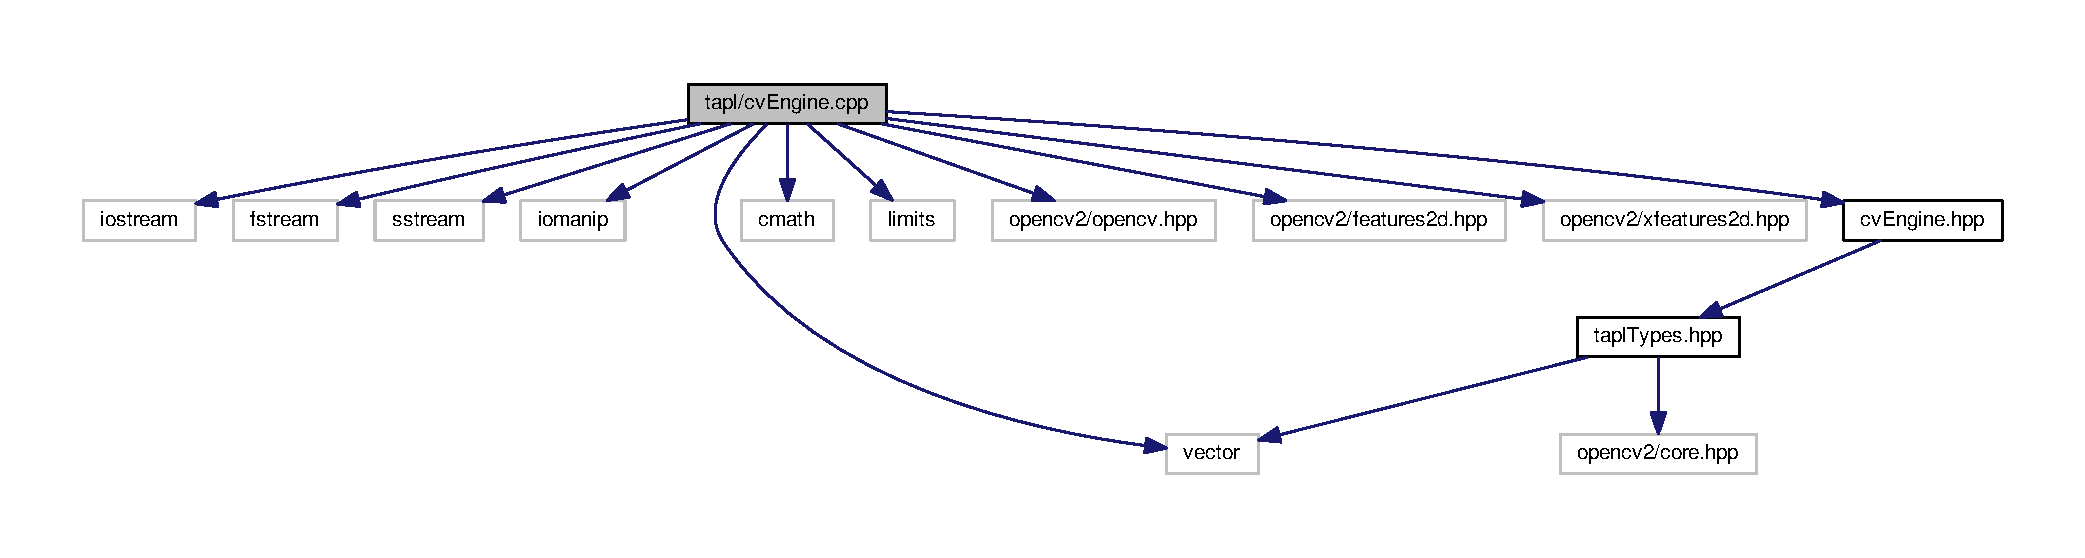
\includegraphics[width=350pt]{cvEngine_8cpp__incl}
\end{center}
\end{figure}
\subsection*{Functions}
\begin{DoxyCompactItemize}
\item 
void \hyperlink{cvEngine_8cpp_a7f717198f1e528db1077f706c9f9c515}{rodrigues2euler} (cv\+::\+Mat \&R, float \&roll, float \&pitch, float \&yaw)
\end{DoxyCompactItemize}


\subsection{Function Documentation}
\index{cv\+Engine.\+cpp@{cv\+Engine.\+cpp}!rodrigues2euler@{rodrigues2euler}}
\index{rodrigues2euler@{rodrigues2euler}!cv\+Engine.\+cpp@{cv\+Engine.\+cpp}}
\subsubsection[{\texorpdfstring{rodrigues2euler(cv\+::\+Mat \&\+R, float \&roll, float \&pitch, float \&yaw)}{rodrigues2euler(cv::Mat &R, float &roll, float &pitch, float &yaw)}}]{\setlength{\rightskip}{0pt plus 5cm}void rodrigues2euler (
\begin{DoxyParamCaption}
\item[{cv\+::\+Mat \&}]{R, }
\item[{float \&}]{roll, }
\item[{float \&}]{pitch, }
\item[{float \&}]{yaw}
\end{DoxyParamCaption}
)}\hypertarget{cvEngine_8cpp_a7f717198f1e528db1077f706c9f9c515}{}\label{cvEngine_8cpp_a7f717198f1e528db1077f706c9f9c515}
Rodrigues to Euler angle conversion 

Definition at line 408 of file cv\+Engine.\+cpp.



Here is the caller graph for this function\+:\nopagebreak
\begin{figure}[H]
\begin{center}
\leavevmode
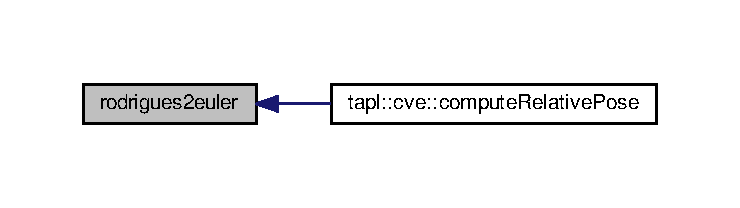
\includegraphics[width=350pt]{cvEngine_8cpp_a7f717198f1e528db1077f706c9f9c515_icgraph}
\end{center}
\end{figure}



\hypertarget{cvEngine_8hpp}{}\doxysection{tapl/cve/cv\+Engine.hpp File Reference}
\label{cvEngine_8hpp}\index{tapl/cve/cvEngine.hpp@{tapl/cve/cvEngine.hpp}}


This file provides A\+P\+Is for computer vision related functions.  


{\ttfamily \#include \char`\"{}tapl/common/tapl\+Types.\+hpp\char`\"{}}\newline
Include dependency graph for cv\+Engine.\+hpp\+:
\nopagebreak
\begin{figure}[H]
\begin{center}
\leavevmode
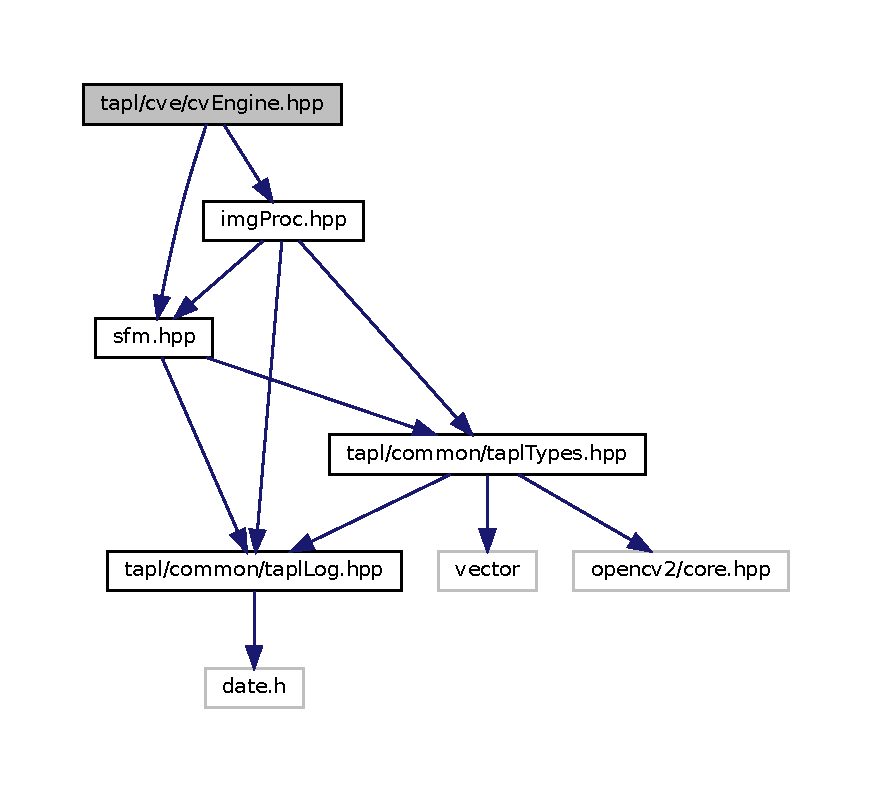
\includegraphics[width=255pt]{cvEngine_8hpp__incl}
\end{center}
\end{figure}
This graph shows which files directly or indirectly include this file\+:
\nopagebreak
\begin{figure}[H]
\begin{center}
\leavevmode
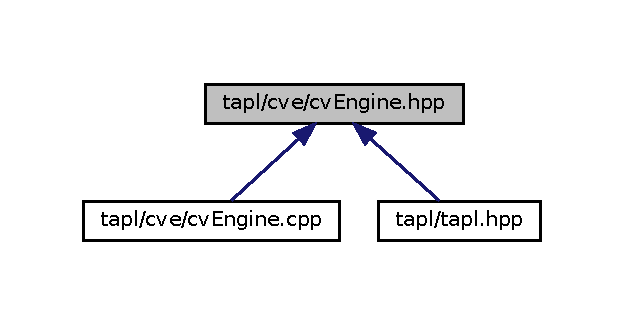
\includegraphics[width=300pt]{cvEngine_8hpp__dep__incl}
\end{center}
\end{figure}
\doxysubsection*{Namespaces}
\begin{DoxyCompactItemize}
\item 
 \mbox{\hyperlink{namespacetapl}{tapl}}
\item 
 \mbox{\hyperlink{namespacetapl_1_1cve}{tapl\+::cve}}
\end{DoxyCompactItemize}
\doxysubsection*{Functions}
\begin{DoxyCompactItemize}
\item 
\mbox{\hyperlink{namespacetapl_a196ce1d5bf399fc26f03797e6a8d03ff}{tapl\+::\+Result\+Code}} \mbox{\hyperlink{namespacetapl_1_1cve_ad74b56dc35c6a902870725543d5df419}{tapl\+::cve\+::detect\+Keypoints}} (cv\+::\+Mat \&img, std\+::vector$<$ cv\+::\+Key\+Point $>$ \&keypoints, std\+::string detector\+Type=\char`\"{}F\+A\+ST\char`\"{})
\begin{DoxyCompactList}\small\item\em This function detects keypoints in an image. \end{DoxyCompactList}\item 
\mbox{\hyperlink{namespacetapl_a196ce1d5bf399fc26f03797e6a8d03ff}{tapl\+::\+Result\+Code}} \mbox{\hyperlink{namespacetapl_1_1cve_a02712316099758c2b4d0bb0e4e5dc219}{tapl\+::cve\+::extract\+Descriptors}} (cv\+::\+Mat \&img, std\+::vector$<$ cv\+::\+Key\+Point $>$ \&keypoints, cv\+::\+Mat \&descriptors, std\+::string descriptor\+Type=\char`\"{}B\+R\+I\+SK\char`\"{})
\begin{DoxyCompactList}\small\item\em This function extracts keypoints descriptors in an image. \end{DoxyCompactList}\item 
\mbox{\hyperlink{namespacetapl_a196ce1d5bf399fc26f03797e6a8d03ff}{tapl\+::\+Result\+Code}} \mbox{\hyperlink{namespacetapl_1_1cve_ae2699cc690841efd3b7a3179be1fb889}{tapl\+::cve\+::match\+Descriptors}} (std\+::vector$<$ cv\+::\+Key\+Point $>$ \&k\+Pts\+Source, std\+::vector$<$ cv\+::\+Key\+Point $>$ \&k\+Pts\+Ref, cv\+::\+Mat \&desc\+Source, cv\+::\+Mat \&desc\+Ref, std\+::vector$<$ cv\+::\+D\+Match $>$ \&matches, std\+::string norm\+Type=\char`\"{}N\+O\+R\+M\+\_\+\+H\+A\+M\+M\+I\+NG\char`\"{}, std\+::string matcher\+Type=\char`\"{}M\+A\+T\+\_\+\+BF\char`\"{}, std\+::string selector\+Type=\char`\"{}S\+E\+L\+\_\+\+K\+NN\char`\"{})
\begin{DoxyCompactList}\small\item\em This function performs keypoint descriptor matching. \end{DoxyCompactList}\item 
\mbox{\hyperlink{namespacetapl_a196ce1d5bf399fc26f03797e6a8d03ff}{tapl\+::\+Result\+Code}} \mbox{\hyperlink{namespacetapl_1_1cve_a34cb000d47a121549e81900da9913299}{tapl\+::cve\+::detect\+And\+Match\+Kpts}} (\mbox{\hyperlink{structtapl_1_1DataFrame}{tapl\+::\+Data\+Frame}} \&dframe1, \mbox{\hyperlink{structtapl_1_1DataFrame}{tapl\+::\+Data\+Frame}} \&dframe2)
\begin{DoxyCompactList}\small\item\em This function detects keypoints in two image frames and perform keypoints matching. \end{DoxyCompactList}\item 
\mbox{\hyperlink{namespacetapl_a196ce1d5bf399fc26f03797e6a8d03ff}{tapl\+::\+Result\+Code}} \mbox{\hyperlink{namespacetapl_1_1cve_a8e1c9ef8d5eae6975b5e7e7c360fc1e8}{tapl\+::cve\+::compute\+Fundamental\+Matrix}} (\mbox{\hyperlink{structtapl_1_1DataFrame}{tapl\+::\+Data\+Frame}} \&dframe1, \mbox{\hyperlink{structtapl_1_1DataFrame}{tapl\+::\+Data\+Frame}} \&dframe2)
\begin{DoxyCompactList}\small\item\em This function retrieves fundamental matrix between two images contained within their data frame structure. \end{DoxyCompactList}\item 
\mbox{\hyperlink{namespacetapl_a196ce1d5bf399fc26f03797e6a8d03ff}{tapl\+::\+Result\+Code}} \mbox{\hyperlink{namespacetapl_1_1cve_a30da40f2aa0e434425c7b14f23b59457}{tapl\+::cve\+::compute\+Essential\+Matrix}} (\mbox{\hyperlink{structtapl_1_1DataFrame}{tapl\+::\+Data\+Frame}} \&dframe1, \mbox{\hyperlink{structtapl_1_1DataFrame}{tapl\+::\+Data\+Frame}} \&dframe2, cv\+::\+Mat \&camera\+\_\+matrix)
\begin{DoxyCompactList}\small\item\em This function retrieves essential matrix between two images contained within their data frame structure. \end{DoxyCompactList}\item 
\mbox{\hyperlink{namespacetapl_a196ce1d5bf399fc26f03797e6a8d03ff}{tapl\+::\+Result\+Code}} \mbox{\hyperlink{namespacetapl_1_1cve_ad8314ef8898d3a90c6d93a514bf75d20}{tapl\+::cve\+::compute\+Relative\+Pose}} (\mbox{\hyperlink{structtapl_1_1DataFrame}{tapl\+::\+Data\+Frame}} \&dframe1, \mbox{\hyperlink{structtapl_1_1DataFrame}{tapl\+::\+Data\+Frame}} \&dframe2, cv\+::\+Mat \&camera\+\_\+matrix)
\begin{DoxyCompactList}\small\item\em This function is used to compute the relative camera pose. Pose is computed for second image contained within dframe2 relative to dframe1. \end{DoxyCompactList}\item 
\mbox{\hyperlink{namespacetapl_a196ce1d5bf399fc26f03797e6a8d03ff}{tapl\+::\+Result\+Code}} \mbox{\hyperlink{namespacetapl_1_1cve_aab4041f410589ff960febecf36b3ee2b}{tapl\+::cve\+::stitch\+Panaromic}} (const std\+::vector$<$ cv\+::\+Mat $>$ \&imgs, cv\+::\+Mat \&panoramic\+\_\+img)
\begin{DoxyCompactList}\small\item\em This function is used to stitch multiple images as a panaromic image. \end{DoxyCompactList}\end{DoxyCompactItemize}


\doxysubsection{Detailed Description}
This file provides A\+P\+Is for computer vision related functions. 

\begin{DoxyAuthor}{Author}
Shubham Shrivastava 
\end{DoxyAuthor}

\hypertarget{ptEngine_8cpp}{}\doxysection{tapl/pte/pt\+Engine.cpp File Reference}
\label{ptEngine_8cpp}\index{tapl/pte/ptEngine.cpp@{tapl/pte/ptEngine.cpp}}
{\ttfamily \#include \char`\"{}pt\+Engine.\+hpp\char`\"{}}\newline
{\ttfamily \#include $<$Eigen/\+Dense$>$}\newline
Include dependency graph for pt\+Engine.\+cpp\+:
\nopagebreak
\begin{figure}[H]
\begin{center}
\leavevmode
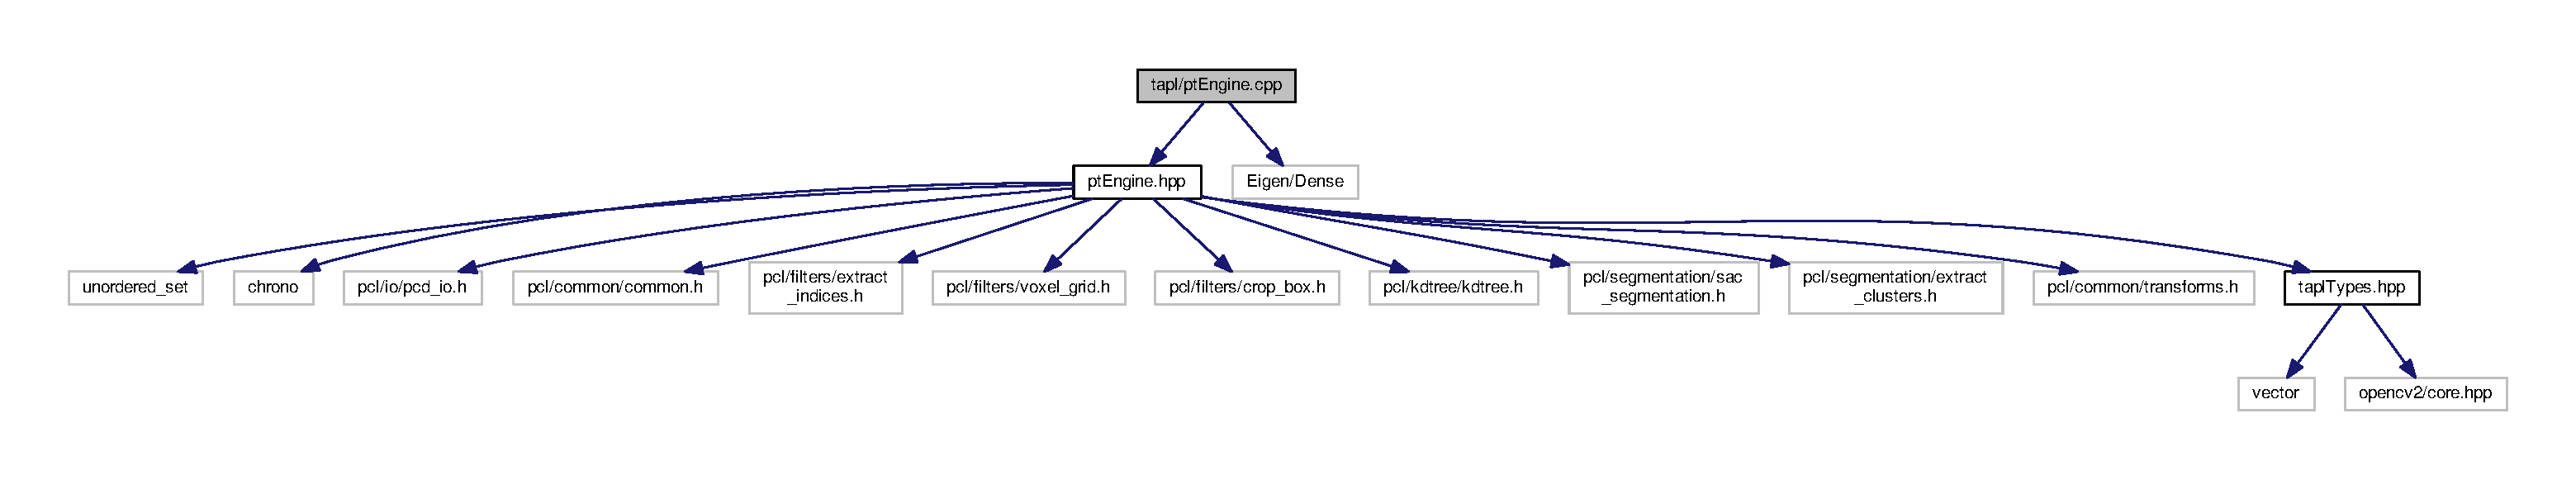
\includegraphics[width=350pt]{ptEngine_8cpp__incl}
\end{center}
\end{figure}
\doxysubsection*{Namespaces}
\begin{DoxyCompactItemize}
\item 
 \mbox{\hyperlink{namespacetapl}{tapl}}
\item 
 \mbox{\hyperlink{namespacetapl_1_1pte}{tapl\+::pte}}
\end{DoxyCompactItemize}
\doxysubsection*{Functions}
\begin{DoxyCompactItemize}
\item 
cv\+::\+Mat \mbox{\hyperlink{namespacetapl_1_1pte_a874efe99ea9c6366ae0c0329554ad200}{tapl\+::pte\+::world2\+Cam\+Rotation}} ()
\begin{DoxyCompactList}\small\item\em returns world to camera rotation matrix \end{DoxyCompactList}\item 
{\footnotesize template$<$typename PointT $>$ }\\void \mbox{\hyperlink{namespacetapl_1_1pte_a928126360beb48c632ff331ca560a1b0}{tapl\+::pte\+::world2\+Cam\+Coordinate}} (PointT \&point)
\begin{DoxyCompactList}\small\item\em affine transform on a point \end{DoxyCompactList}\end{DoxyCompactItemize}

\hypertarget{ptEngine_8hpp}{}\doxysection{tapl/pt\+Engine.hpp File Reference}
\label{ptEngine_8hpp}\index{tapl/ptEngine.hpp@{tapl/ptEngine.hpp}}


This file provides A\+P\+Is for all point related functions. This includes point-\/cloud processing, point transformations, 


{\ttfamily \#include $<$unordered\+\_\+set$>$}\newline
{\ttfamily \#include $<$chrono$>$}\newline
{\ttfamily \#include $<$pcl/io/pcd\+\_\+io.\+h$>$}\newline
{\ttfamily \#include $<$pcl/common/common.\+h$>$}\newline
{\ttfamily \#include $<$pcl/filters/extract\+\_\+indices.\+h$>$}\newline
{\ttfamily \#include $<$pcl/filters/voxel\+\_\+grid.\+h$>$}\newline
{\ttfamily \#include $<$pcl/filters/crop\+\_\+box.\+h$>$}\newline
{\ttfamily \#include $<$pcl/kdtree/kdtree.\+h$>$}\newline
{\ttfamily \#include $<$pcl/segmentation/sac\+\_\+segmentation.\+h$>$}\newline
{\ttfamily \#include $<$pcl/segmentation/extract\+\_\+clusters.\+h$>$}\newline
{\ttfamily \#include $<$pcl/common/transforms.\+h$>$}\newline
{\ttfamily \#include \char`\"{}tapl\+Types.\+hpp\char`\"{}}\newline
Include dependency graph for pt\+Engine.\+hpp\+:
\nopagebreak
\begin{figure}[H]
\begin{center}
\leavevmode
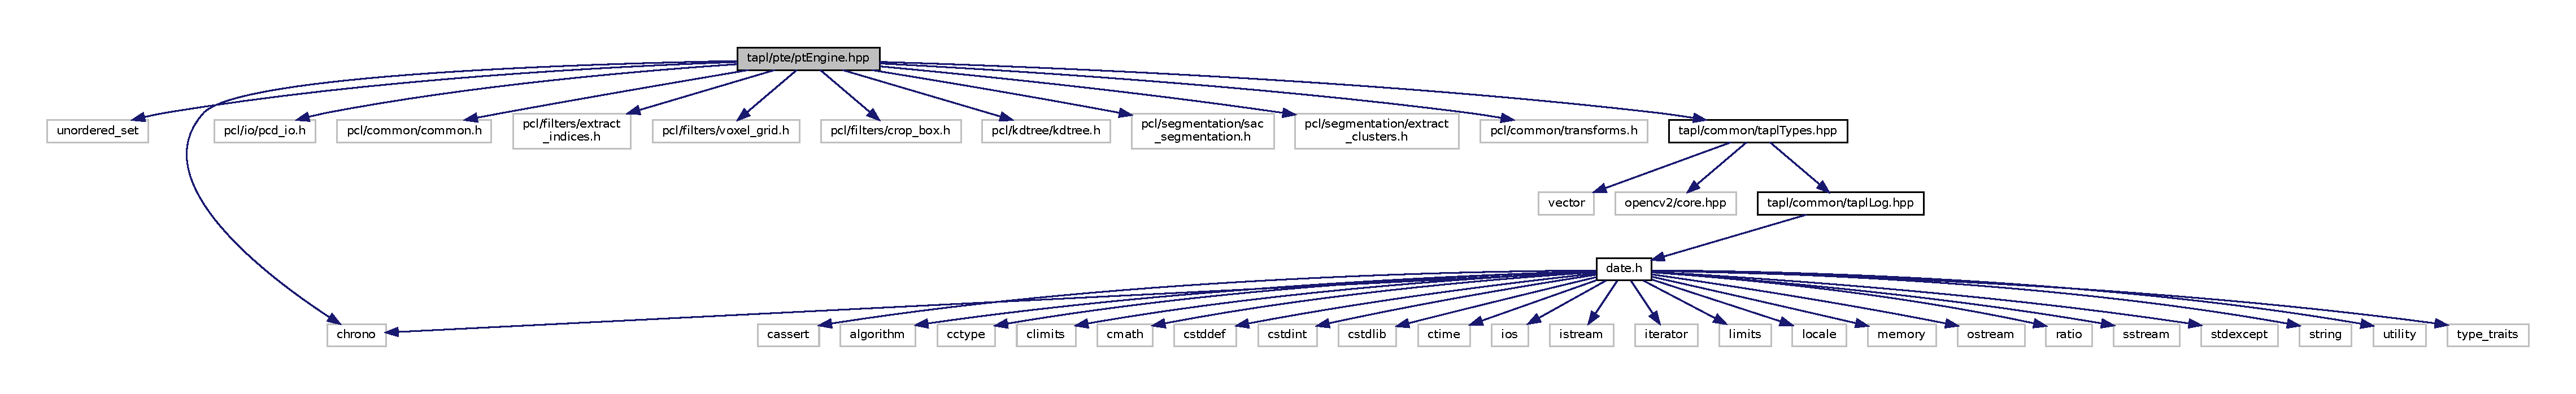
\includegraphics[width=350pt]{ptEngine_8hpp__incl}
\end{center}
\end{figure}
This graph shows which files directly or indirectly include this file\+:
\nopagebreak
\begin{figure}[H]
\begin{center}
\leavevmode
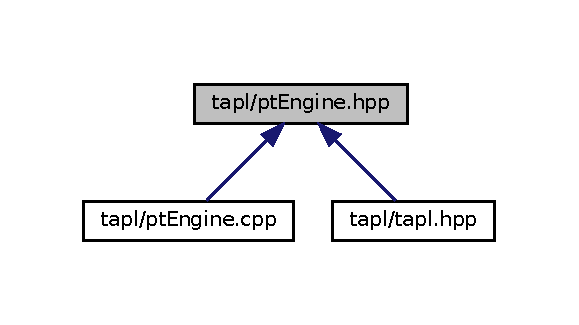
\includegraphics[width=278pt]{ptEngine_8hpp__dep__incl}
\end{center}
\end{figure}
\doxysubsection*{Data Structures}
\begin{DoxyCompactItemize}
\item 
class \mbox{\hyperlink{classtapl_1_1pte_1_1Line}{tapl\+::pte\+::\+Line$<$ Point\+T $>$}}
\item 
class \mbox{\hyperlink{classtapl_1_1pte_1_1Plane}{tapl\+::pte\+::\+Plane$<$ Point\+T $>$}}
\item 
struct \mbox{\hyperlink{structtapl_1_1pte_1_1Node}{tapl\+::pte\+::\+Node}}
\item 
struct \mbox{\hyperlink{structtapl_1_1pte_1_1KdTree}{tapl\+::pte\+::\+Kd\+Tree}}
\item 
class \mbox{\hyperlink{classtapl_1_1pte_1_1EuclideanCluster}{tapl\+::pte\+::\+Euclidean\+Cluster}}
\end{DoxyCompactItemize}
\doxysubsection*{Namespaces}
\begin{DoxyCompactItemize}
\item 
 \mbox{\hyperlink{namespacetapl}{tapl}}
\item 
 \mbox{\hyperlink{namespacetapl_1_1pte}{tapl\+::pte}}
\end{DoxyCompactItemize}
\doxysubsection*{Functions}
\begin{DoxyCompactItemize}
\item 
float \mbox{\hyperlink{ptEngine_8hpp_af587759c004d4f86b1c5821066cca76a}{degrees\+To\+Radians}} (float angle\+Degrees)
\item 
float \mbox{\hyperlink{ptEngine_8hpp_a4ac6c9ad7b92e0e724726603b7714c88}{radians\+To\+Degrees}} (float angle\+Radians)
\item 
cv\+::\+Mat \mbox{\hyperlink{namespacetapl_1_1pte_a874efe99ea9c6366ae0c0329554ad200}{tapl\+::pte\+::world2\+Cam\+Rotation}} ()
\begin{DoxyCompactList}\small\item\em returns world to camera rotation matrix \end{DoxyCompactList}\item 
{\footnotesize template$<$typename PointT $>$ }\\void \mbox{\hyperlink{namespacetapl_1_1pte_a928126360beb48c632ff331ca560a1b0}{tapl\+::pte\+::world2\+Cam\+Coordinate}} (PointT \&point)
\begin{DoxyCompactList}\small\item\em affine transform on a point \end{DoxyCompactList}\item 
{\footnotesize template$<$typename PointT $>$ }\\void \mbox{\hyperlink{namespacetapl_1_1pte_a48c0b0806659501276e0b33042e2fa5b}{tapl\+::pte\+::downsample\+Cloud}} (typename pcl\+::\+Point\+Cloud$<$ PointT $>$\+::Ptr cloud, float resolution)
\begin{DoxyCompactList}\small\item\em Downsample point-\/cloud. \end{DoxyCompactList}\item 
{\footnotesize template$<$typename PointT $>$ }\\void \mbox{\hyperlink{namespacetapl_1_1pte_adaa36d31de7cd145e875901dfa13a616}{tapl\+::pte\+::crop\+Cloud}} (typename pcl\+::\+Point\+Cloud$<$ PointT $>$\+::Ptr cloud, float x\+\_\+min, float x\+\_\+max, float y\+\_\+min, float y\+\_\+max, float z\+\_\+min, float z\+\_\+max)
\begin{DoxyCompactList}\small\item\em Crop point-\/cloud given a region of interest. \end{DoxyCompactList}\item 
{\footnotesize template$<$typename PointT $>$ }\\\mbox{\hyperlink{namespacetapl_a196ce1d5bf399fc26f03797e6a8d03ff}{tapl\+::\+Result\+Code}} \mbox{\hyperlink{namespacetapl_1_1pte_aa4fc09affe62218081e85ed5818bf2ef}{tapl\+::pte\+::segment\+Plane}} (typename pcl\+::\+Point\+Cloud$<$ PointT $>$\+::Ptr cloud, std\+::pair$<$ typename pcl\+::\+Point\+Cloud$<$ PointT $>$\+::Ptr, typename pcl\+::\+Point\+Cloud$<$ PointT $>$\+::Ptr $>$ \&seg\+Result, int max\+Iterations, float distance\+Threshold, bool use\+P\+CL=false)
\begin{DoxyCompactList}\small\item\em This function segments a plane within a point-\/cloud. Points within the plane are inliers and other points are outliers. It populates two separate point-\/clouds corresponding to inliers and outliers. \end{DoxyCompactList}\item 
{\footnotesize template$<$typename PointT $>$ }\\std\+::vector$<$ typename pcl\+::\+Point\+Cloud$<$ PointT $>$\+::Ptr $>$ \mbox{\hyperlink{namespacetapl_1_1pte_a69e06eaa64248177550033adb709fb3d}{tapl\+::pte\+::euclidean\+Clustering}} (typename pcl\+::\+Point\+Cloud$<$ PointT $>$\+::Ptr cloud, float cluster\+Tolerance, int min\+Num\+Points, int max\+Num\+Points, bool use\+P\+CL=false)
\begin{DoxyCompactList}\small\item\em Perform euclidean clustering within a point-\/cloud. Returns a vector of cluster clouds. \end{DoxyCompactList}\item 
{\footnotesize template$<$typename PointT $>$ }\\\mbox{\hyperlink{structtapl_1_1BBox3d}{tapl\+::\+B\+Box3d}} \mbox{\hyperlink{namespacetapl_1_1pte_ac4b4a53485d62466140d43448496536b}{tapl\+::pte\+::get\+Bounding\+Box}} (typename pcl\+::\+Point\+Cloud$<$ PointT $>$\+::Ptr cloud\+Cluster)
\begin{DoxyCompactList}\small\item\em This function is used to obtain bounding-\/box for a cluster of points. \end{DoxyCompactList}\end{DoxyCompactItemize}


\doxysubsection{Detailed Description}
This file provides A\+P\+Is for all point related functions. This includes point-\/cloud processing, point transformations,

\begin{DoxyAuthor}{Author}
Shubham Shrivastava 
\end{DoxyAuthor}


\doxysubsection{Function Documentation}
\mbox{\Hypertarget{ptEngine_8hpp_af587759c004d4f86b1c5821066cca76a}\label{ptEngine_8hpp_af587759c004d4f86b1c5821066cca76a}} 
\index{ptEngine.hpp@{ptEngine.hpp}!degreesToRadians@{degreesToRadians}}
\index{degreesToRadians@{degreesToRadians}!ptEngine.hpp@{ptEngine.hpp}}
\doxysubsubsection{\texorpdfstring{degreesToRadians()}{degreesToRadians()}}
{\footnotesize\ttfamily float degrees\+To\+Radians (\begin{DoxyParamCaption}\item[{float}]{angle\+Degrees }\end{DoxyParamCaption})\hspace{0.3cm}{\ttfamily [inline]}}



Definition at line 27 of file pt\+Engine.\+hpp.

Here is the caller graph for this function\+:
\nopagebreak
\begin{figure}[H]
\begin{center}
\leavevmode
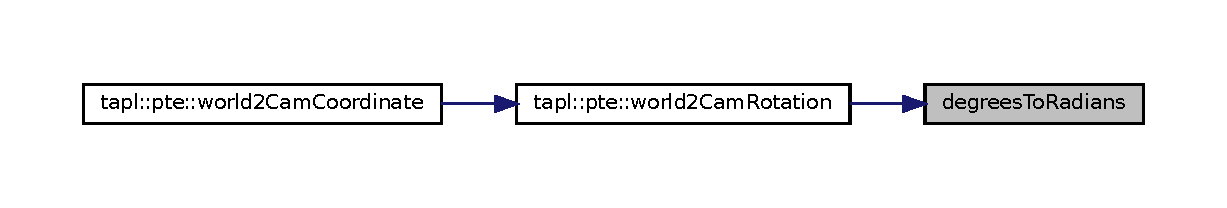
\includegraphics[width=350pt]{ptEngine_8hpp_af587759c004d4f86b1c5821066cca76a_icgraph}
\end{center}
\end{figure}
\mbox{\Hypertarget{ptEngine_8hpp_a4ac6c9ad7b92e0e724726603b7714c88}\label{ptEngine_8hpp_a4ac6c9ad7b92e0e724726603b7714c88}} 
\index{ptEngine.hpp@{ptEngine.hpp}!radiansToDegrees@{radiansToDegrees}}
\index{radiansToDegrees@{radiansToDegrees}!ptEngine.hpp@{ptEngine.hpp}}
\doxysubsubsection{\texorpdfstring{radiansToDegrees()}{radiansToDegrees()}}
{\footnotesize\ttfamily float radians\+To\+Degrees (\begin{DoxyParamCaption}\item[{float}]{angle\+Radians }\end{DoxyParamCaption})\hspace{0.3cm}{\ttfamily [inline]}}



Definition at line 28 of file pt\+Engine.\+hpp.


\hypertarget{ringBuffer_8hpp}{}\section{tapl/ring\+Buffer.hpp File Reference}
\label{ringBuffer_8hpp}\index{tapl/ring\+Buffer.\+hpp@{tapl/ring\+Buffer.\+hpp}}


This file provides an implementation of a ring buffer.  


{\ttfamily \#include $<$iostream$>$}\\*
{\ttfamily \#include $<$algorithm$>$}\\*
Include dependency graph for ring\+Buffer.\+hpp\+:\nopagebreak
\begin{figure}[H]
\begin{center}
\leavevmode
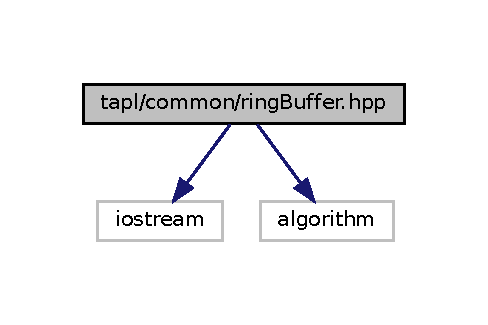
\includegraphics[width=208pt]{ringBuffer_8hpp__incl}
\end{center}
\end{figure}
This graph shows which files directly or indirectly include this file\+:\nopagebreak
\begin{figure}[H]
\begin{center}
\leavevmode
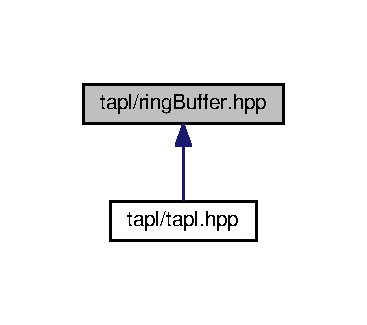
\includegraphics[width=176pt]{ringBuffer_8hpp__dep__incl}
\end{center}
\end{figure}
\subsection*{Data Structures}
\begin{DoxyCompactItemize}
\item 
class \hyperlink{classtapl_1_1RingBuffer}{tapl\+::\+Ring\+Buffer$<$ T $>$}
\begin{DoxyCompactList}\small\item\em Ring Buffer. \end{DoxyCompactList}\end{DoxyCompactItemize}
\subsection*{Namespaces}
\begin{DoxyCompactItemize}
\item 
 \hyperlink{namespacetapl}{tapl}
\end{DoxyCompactItemize}


\subsection{Detailed Description}
This file provides an implementation of a ring buffer. 

\begin{DoxyAuthor}{Author}
Shubham Shrivastava 
\end{DoxyAuthor}

\hypertarget{tapl_8hpp}{}\doxysection{tapl/tapl.hpp File Reference}
\label{tapl_8hpp}\index{tapl/tapl.hpp@{tapl/tapl.hpp}}


This is the main header file which exposes all the available A\+P\+Is to users.  


{\ttfamily \#include \char`\"{}tapl/common/tapl\+Types.\+hpp\char`\"{}}\newline
{\ttfamily \#include \char`\"{}tapl/common/ring\+Buffer.\+hpp\char`\"{}}\newline
{\ttfamily \#include \char`\"{}tapl/cve/cv\+Engine.\+hpp\char`\"{}}\newline
{\ttfamily \#include \char`\"{}tapl/pte/pt\+Engine.\+hpp\char`\"{}}\newline
{\ttfamily \#include \char`\"{}tapl/viz/visualization.\+hpp\char`\"{}}\newline
Include dependency graph for tapl.\+hpp\+:
\nopagebreak
\begin{figure}[H]
\begin{center}
\leavevmode
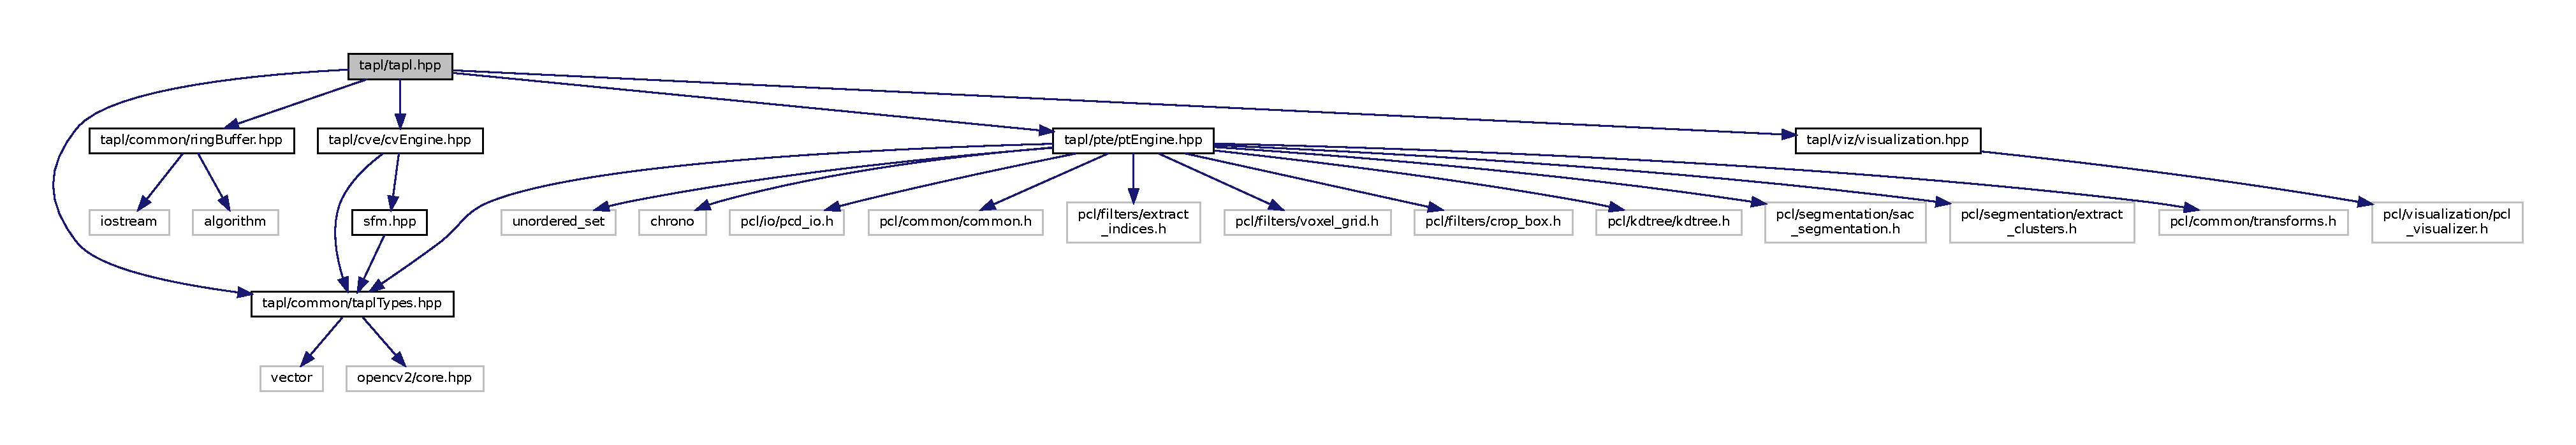
\includegraphics[width=350pt]{tapl_8hpp__incl}
\end{center}
\end{figure}


\doxysubsection{Detailed Description}
This is the main header file which exposes all the available A\+P\+Is to users. 

\begin{DoxyAuthor}{Author}
Shubham Shrivastava 
\end{DoxyAuthor}

\hypertarget{taplTypes_8hpp}{}\doxysection{tapl/common/tapl\+Types.hpp File Reference}
\label{taplTypes_8hpp}\index{tapl/common/taplTypes.hpp@{tapl/common/taplTypes.hpp}}


This file provides type definitions used throughout this library.  


{\ttfamily \#include $<$vector$>$}\newline
{\ttfamily \#include $<$opencv2/core.\+hpp$>$}\newline
{\ttfamily \#include \char`\"{}tapl/common/tapl\+Log.\+hpp\char`\"{}}\newline
Include dependency graph for tapl\+Types.\+hpp\+:
\nopagebreak
\begin{figure}[H]
\begin{center}
\leavevmode
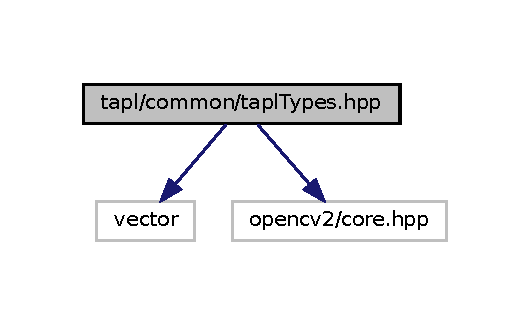
\includegraphics[width=350pt]{taplTypes_8hpp__incl}
\end{center}
\end{figure}
This graph shows which files directly or indirectly include this file\+:\nopagebreak
\begin{figure}[H]
\begin{center}
\leavevmode
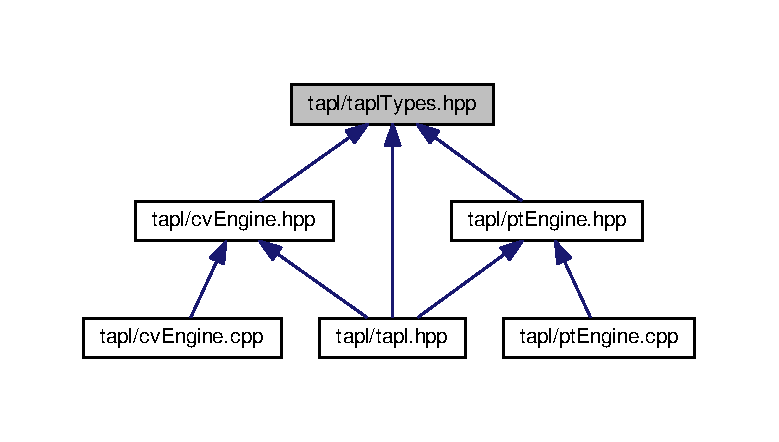
\includegraphics[width=350pt]{taplTypes_8hpp__dep__incl}
\end{center}
\end{figure}
\doxysubsection*{Data Structures}
\begin{DoxyCompactItemize}
\item 
struct \mbox{\hyperlink{structtapl_1_1Point3d}{tapl\+::\+Point3d}}
\begin{DoxyCompactList}\small\item\em 3D Point \end{DoxyCompactList}\item 
struct \mbox{\hyperlink{structtapl_1_1BBox3d}{tapl\+::\+B\+Box3d}}
\begin{DoxyCompactList}\small\item\em 3D Bounding-\/\+Box \end{DoxyCompactList}\item 
struct \mbox{\hyperlink{structtapl_1_1Pose6dof}{tapl\+::\+Pose6dof}}
\begin{DoxyCompactList}\small\item\em 6-\/D\+OF Camera Pose \end{DoxyCompactList}\item 
struct \mbox{\hyperlink{structtapl_1_1CameraFrame}{tapl\+::\+Camera\+Frame}}
\begin{DoxyCompactList}\small\item\em represents a camera frame \end{DoxyCompactList}\item 
struct \mbox{\hyperlink{structtapl_1_1DataFrame}{tapl\+::\+Data\+Frame}}
\begin{DoxyCompactList}\small\item\em represents the available sensor information at the same time instance \end{DoxyCompactList}\end{DoxyCompactItemize}
\doxysubsection*{Namespaces}
\begin{DoxyCompactItemize}
\item 
 \mbox{\hyperlink{namespacetapl}{tapl}}
\end{DoxyCompactItemize}
\doxysubsection*{Enumerations}
\begin{DoxyCompactItemize}
\item 
enum \mbox{\hyperlink{namespacetapl_a196ce1d5bf399fc26f03797e6a8d03ff}{tapl\+::\+Result\+Code}} \{ \mbox{\hyperlink{namespacetapl_a196ce1d5bf399fc26f03797e6a8d03ffaa6e243674a964518a62bdda7f20f6453}{tapl\+::\+F\+A\+I\+L\+U\+RE}} =-\/1, 
\mbox{\hyperlink{namespacetapl_a196ce1d5bf399fc26f03797e6a8d03ffafbdd78b1e8654e11461f37fea68c6195}{tapl\+::\+S\+U\+C\+C\+E\+SS}} =0
 \}
\begin{DoxyCompactList}\small\item\em Result code enumerations. \end{DoxyCompactList}\end{DoxyCompactItemize}


\doxysubsection{Detailed Description}
This file provides type definitions used throughout this library. 

\begin{DoxyAuthor}{Author}
Shubham Shrivastava 
\end{DoxyAuthor}

\hypertarget{visualization_8hpp}{}\doxysection{tapl/viz/visualization.hpp File Reference}
\label{visualization_8hpp}\index{tapl/viz/visualization.hpp@{tapl/viz/visualization.hpp}}


This file provides A\+P\+Is for visualization.  


{\ttfamily \#include $<$pcl/visualization/pcl\+\_\+visualizer.\+h$>$}\newline
Include dependency graph for visualization.\+hpp\+:\nopagebreak
\begin{figure}[H]
\begin{center}
\leavevmode
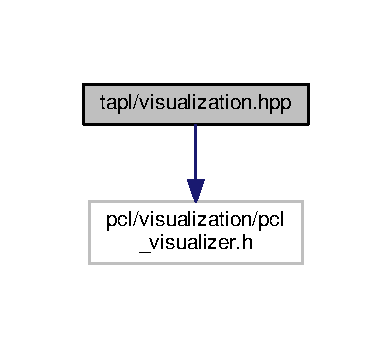
\includegraphics[width=219pt]{visualization_8hpp__incl}
\end{center}
\end{figure}
This graph shows which files directly or indirectly include this file\+:\nopagebreak
\begin{figure}[H]
\begin{center}
\leavevmode
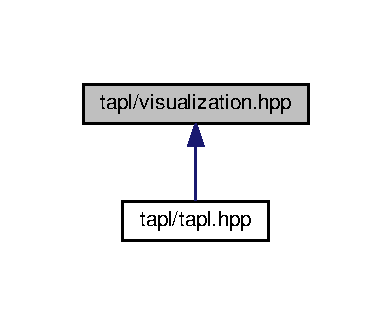
\includegraphics[width=350pt]{visualization_8hpp__dep__incl}
\end{center}
\end{figure}
\doxysubsection*{Data Structures}
\begin{DoxyCompactItemize}
\item 
class \mbox{\hyperlink{classtapl_1_1viz_1_1Visualizer}{tapl\+::viz\+::\+Visualizer}}
\begin{DoxyCompactList}\small\item\em Implementation of the visualizer class. \end{DoxyCompactList}\end{DoxyCompactItemize}
\doxysubsection*{Namespaces}
\begin{DoxyCompactItemize}
\item 
 \mbox{\hyperlink{namespacetapl}{tapl}}
\item 
 \mbox{\hyperlink{namespacetapl_1_1viz}{tapl\+::viz}}
\end{DoxyCompactItemize}
\doxysubsection*{Enumerations}
\begin{DoxyCompactItemize}
\item 
enum \mbox{\hyperlink{namespacetapl_1_1viz_a99e496921984514dbc7bcef809f50150}{tapl\+::viz\+::\+Camera\+Angle}} \{ \mbox{\hyperlink{namespacetapl_1_1viz_a99e496921984514dbc7bcef809f50150a361bb774c1715ed6be67552bd2aac36e}{tapl\+::viz\+::\+XY}}, 
\mbox{\hyperlink{namespacetapl_1_1viz_a99e496921984514dbc7bcef809f50150a9aa35eea1fe8f4b45a0b02a8b5048cfa}{tapl\+::viz\+::\+Top\+Down}}, 
\mbox{\hyperlink{namespacetapl_1_1viz_a99e496921984514dbc7bcef809f50150aa268beeef2cb7c134c70cc8fc05b7045}{tapl\+::viz\+::\+Side}}, 
\mbox{\hyperlink{namespacetapl_1_1viz_a99e496921984514dbc7bcef809f50150a85d72fbe54240f98c1ed1ccd5fe8b7d9}{tapl\+::viz\+::\+F\+PS}}
 \}
\begin{DoxyCompactList}\small\item\em Enumerations for camera view angle. \end{DoxyCompactList}\end{DoxyCompactItemize}


\doxysubsection{Detailed Description}
This file provides A\+P\+Is for visualization. 

\begin{DoxyAuthor}{Author}
Shubham Shrivastava 
\end{DoxyAuthor}

%--- End generated contents ---

% Index
\backmatter
\newpage
\phantomsection
\clearemptydoublepage
\addcontentsline{toc}{chapter}{Index}
\printindex

\end{document}
